%!TEX TS-program = pdflatex
% dissertation.tex -- main dissertation file
%
% Wisconsin dissertation template
% Copyright (c) 2008-2009 William C. Benton.  All rights reserved.
%
% This program can redistributed and/or modified under the terms
% of the LaTeX Project Public License Distributed from CTAN
% archives in directory macros/latex/base/lppl.txt; either
% version 1 of the License, or (at your option) any later version.
%
% This program includes other software that is licensed under the
% terms of the LPPL and the Perl Artistic License; see README for details.
%
% You, the user, still hold the copyright to any document you produce
% with this software (like your dissertation).
%

%%% You'll want ``oneside'' for the deposit version, but probably not for any versions that don't need to meet the UW requirements
\documentclass[12pt,oneside,letterpaper]{memoir}

% preamble.tex -- packages to include
%
% Wisconsin dissertation template
% Copyright (c) 2008 William C. Benton.  All rights reserved.
%
% This program can redistributed and/or modified under the terms
% of the LaTeX Project Public License Distributed from CTAN
% archives in directory macros/latex/base/lppl.txt; either
% version 1 of the License, or (at your option) any later version.
%
% This program includes other software that is licensed under the
% terms of the LPPL and the Perl Artistic License; see README for details.
%
% You, the user, still hold the copyright to any document you produce
% with this software (like your dissertation).

%% You should use natbib
\IfFileExists{natbib.sty}{%
\usepackage[numbers,sort]{natbib}%
}{}

%% You probably need appendix, if you want appendices
\IfFileExists{appendix.sty}{%
\usepackage{appendix}%
}{}

%% the spacing in memoir is weird, you'll need to use this
\DisemulatePackage{setspace}
\usepackage[onehalfspacing]{setspace}

%% List setup; the ``hanglist`` environment will allow you to have
%% nicely-typeset enumerated lists (i.e. with the numbers hanging in
%% the margins).  You need at least version 2.1 of enumitem.sty.  If
%% you don't have enumitem installed at all, hanglist will just be an
%% alias for enumerate.
\IfFileExists{enumitem.sty}{%
\usepackage[loadonly]{enumitem}[2007/06/30]%
\newlist{hanglist}{enumerate}{1}% 
\setlist[hanglist]{label=\arabic*.}%
\setlist[hanglist,1]{leftmargin=0pt}%
}{%
\newenvironment{hanglist}{\begin{enumerate}}{\end{enumerate}}%
}

%% Comment out any of these that you don't want
\usepackage{amssymb}
\usepackage{amsmath}
\usepackage{amsthm}
%\usepackage{theorem}
\usepackage{hyperref}

\IfFileExists{mathpartir.sty}{%
\usepackage{mathpartir}%
}{}

%%%%% LISTINGS package and setup
\IfFileExists{listings.sty}{%
\usepackage{listings}%
}{}



%% Get rid of ugly borders around PDF hyperlinks (e.g. for cross-references, bib entries, or URLs)
\hypersetup{pdfborder = 0 0 0}

%% You want microtype.
\IfFileExists{microtype.sty}{%
\usepackage[protrusion=true,expansion=true]{microtype}%
}{}

%\pagestyle{thesisdraft}

% Surround parts of graphics with box
\usepackage{boxedminipage}

%% booktabs (thx to Nate Rosenblum for bringing this beautiful package
%% to my attention)
\IfFileExists{booktabs.sty}{%
\usepackage{booktabs}%
}{}

% This is now the recommended way for checking for PDFLaTeX:
\usepackage{ifpdf}

%% Avoid ugly "Type 3" fonts
\usepackage{lmodern}
\usepackage[LY1]{fontenc}

%% Substitute your favorite serif and sans fonts here....
\IfFileExists{tgpagella.sty}{%
% TeX Gyre pagella, like Palatino
\usepackage{tgpagella}%
}{}

\usepackage[LY1]{eulervm}

\ifpdf
\usepackage[pdftex]{graphicx}
\else
\usepackage{graphicx}
\fi

\usepackage{makeidx}
\makeindex

{\theoremstyle{plain}
\newtheorem{thm}{Theorem}[chapter]
\newtheorem{cor}[thm]{Corollary}
\newtheorem{define}[thm]{Definition}
\newtheorem{exmpl}[thm]{Example}
}
{\theoremstyle{remark}
\newtheorem{rmk}[thm]{Remark}
}

\newtheoremstyle{customsty1}
{3pt}%
{3pt}%
{}% --- body font
{}% --- indent amount
{\bfseries}% --- Theorem head font
{:}% --- Punctuation after head
{.5em}% --- space after head
{}% --- theorem head spec (can be left empty, meaning 'normal')

% Define 'newtheorems' that use ``customsty1''
{\theoremstyle{customsty1} 
}


%%% NB: the ``deposit'' chapter- and page- styles should conform to UW
%%% requirements.  If you are producing a pretty version of your
%%% dissertation for web use later, you will certainly want to make
%%% your own chapter and page styles.

\makechapterstyle{deposit}{%
  \renewcommand{\chapterheadstart}{}
  \renewcommand{\printchaptername}{}
  \renewcommand{\chapternamenum}{}
  \renewcommand{\printchapternum}{\parbox{2em}{\MakeLowercase{\Large\scshape\thechapter{}}} }
  \renewcommand{\afterchapternum}{}
  \renewcommand{\printchaptertitle}[1]{%
  \raggedright\Large\scshape\MakeLowercase{##1}}
  \renewcommand{\afterchaptertitle}{%
  \vskip\onelineskip \hrule\vskip\onelineskip}
}

\makepagestyle{deposit}
 
\makeatletter
 
\renewcommand{\chaptermark}[1]{\markboth{#1}{}}
\renewcommand{\sectionmark}[1]{\markboth{#1}{}}
 
\makeevenfoot{deposit}{}{}{}
\makeoddfoot{deposit}{}{}{}
\makeevenhead{deposit}{\thepage}{}{}
\makeoddhead{deposit}{}{}{\thepage}
\makeatother

%%% set up page numbering for chapter pages to satisfy UW requirements
%%% NB: You will want to delete until the ``SNIP'' mark if you are
%%% making a ``nice'' copy
\copypagestyle{chapter}{plain}
\makeoddfoot{chapter}{}{}{}
\makeevenhead{chapter}{\thepage}{}{}
\makeoddhead{chapter}{}{}{\thepage}
%%% SNIP

%%% bib nonsense
\makeatletter
\newenvironment{wb-bib}[1]{%
  \chapter*{references}
\ifnobibintoc\else 
\phantomsection 
\addcontentsline{toc}{chapter}{References} 
\fi 
\prebibhook
  \begin{bibitemlist}{#1}}{\end{bibitemlist}\postbibhook}

\AtBeginDocument{%
  \@ifpackageloaded{natbib}{% natbib is loaded
    \addtodef{\endthebibliography}{}{\vskip-\lastskip\postbibhook}
    \@ifpackagewith{natbib}{sectionbib}{% with sectionbib option
      \renewcommand{\bibsection}{\@memb@bsec}}%
      {\renewcommand{\bibsection}{\@memb@bchap}}}%
  {}
  \@ifpackagewith{chapterbib}{sectionbib}{%
    \renewcommand{\sectionbib}[2]{}
    \renewcommand{\bibsection}{\@memb@bsec}}{}
}
\makeatother

% defs.tex -- wbepi environment for chapter epigraphs and other useful defs.
%
% Wisconsin dissertation template
% Copyright (c) 2008 William C. Benton.  All rights reserved.
%
% This program can redistributed and/or modified under the terms
% of the LaTeX Project Public License Distributed from CTAN
% archives in directory macros/latex/base/lppl.txt; either
% version 1 of the License, or (at your option) any later version.
%
% This program includes other software that is licensed under the
% terms of the LPPL and the Perl Artistic License; see README for details.
%
% You, the user, still hold the copyright to any document you produce
% with this software (like your dissertation).


%% put lstnewenvironment declarations here, if you're using listings

%% end lstnewenvironment declarations

%% I put convenience definitions that will go in several chapters here

%%%%% begin convenience definitions

\makeatletter
\newcommand{\wb@episource}{}
\newenvironment{wbepi}[1]{\begin{quote}\renewcommand{\wb@episource}{#1}\itshape}{\par\upshape \raggedleft --- \textsc{\wb@episource}\\ \end{quote}}
\makeatother

%%%%% SVN
\IfFileExists{svn-multi.sty}{%
\usepackage{svn-multi}%
%%% Uncomment the second one and comment out the first one if you want
%%% to include subversion revision information in each file.
\newcommand{\vcinfo}{}%
%\newcommand{\vcinfo}{\begin{centering}\fbox{\fbox{\parbox{5in}{Author: \svnauthor\\Revision: \svnfilerev\\Last changed on: \svnfiledate\\URL: \svnkw{HeadURL}}}}\\[1em]\end{centering}}%
}{%
\newcommand{\svnidlong}[4]{}%
\newcommand{\svnfilerev}{}%
\newcommand{\svnauthor}{}%
\newcommand{\svnfiledate}{}%
\newcommand{\svnkw}{}%
\newcommand{\vcinfo}{}%
}

%%%%% end convenience definitions

% thesisdefs.tex

% This is mostly adapted from withesis.cls.  The original copyright
% notice for withesis.cls follows, preceded by two percent signs (%%):

%% withesis.cls
%% LaTeX Style file for the University of Wisconsin-Madison Thesis Format
%% Adapted from the Purdue University Thesis Format
%% Originally by Dave Kraynie
%% Edits by Darrell McCauley
%% Adapted to UW-Madison format by Eric Benedict  (Noted with <EB>)
%% Updated to LaTeX2e by Eric Benedict 24 July 00
%% 
%%=============================================================================
%% Licensed under the Perl Artistic License.
%% see: http://www.ctan.org/tex-archive/help/Catalogue/licenses.artistic.html
%% for more info...
%%=============================================================================

% withesis.cls is available from CTAN.  The modifications to this file
% are also licensed under the Perl Artistic License.

% --wb, 2008

\makeatletter

\newcounter {tocpage}
\newcounter {lofpage}
\newcounter {lotpage}
\newcounter {listofheading}

\newcommand\@thesistitlemedskip{0.2in}
\newcommand\@thesistitlebigskip{0.6in}
\newcommand{\degree}[1]{\gdef\@degree{#1}}
\newcommand{\project}{\gdef\@doctype{A masters project report}}
\newcommand{\prelim}{\gdef\@doctype{A preliminary report}}
\newcommand{\thesis}{\gdef\@doctype{A thesis}}
\newcommand{\dissertation}{\gdef\@doctype{A dissertation}}
\newcommand{\department}[1]{\gdef\@department{(#1)}}

\newenvironment{titlepage}
 {\@restonecolfalse\if@twocolumn\@restonecoltrue\onecolumn
  \else \newpage \fi \thispagestyle{empty}
% \c@page\z@ -- deleted: count title page in thesis
}{\if@restonecol\twocolumn \else \newpage \fi}

\gdef\@degree{Doctor of Philosophy}    %Default is PhD
\gdef\@doctype{A dissertation}         %Default is dissertation

\gdef\@department{(Electrical Engineering)} % Default is Electical Engineering
\gdef\@defensedate{01/01/2100}% Default is a long time from now.
\gdef\@committee{
  Jane Doeverything, Professor, Electrical Engineering\\
  John Dosomethings, Associate Professor, Electrical Engineering\\
  }

\renewcommand{\maketitle}{%
  \begin{titlepage}
%-----------------------------------------------------------------------------
% -- The thesis office doesn't like thanks on title page.  Put it in
% -- the acknowledgments.  This is here so you don't have to change
% -- your titlepage when converting from report style. -> from Purdue, but I
%        left it here since it seems compatible with UW-Madison, Eric
%-----------------------------------------------------------------------------
    \def\thanks##1{\typeout{Warning: `thanks' deleted from thesis titlepage.}}
    \let\footnotesize\small \let\footnoterule\relax \setcounter{page}{1}
    \begin{center}
      {\textbf{\expandafter\expandafter{\@title}}} \\[\@thesistitlebigskip]
       by \\[\@thesistitlemedskip]
      \@author \\[\@thesistitlebigskip]
      \@doctype\ submitted in partial fulfillment of \\
      the requirements for the degree of\\[\@thesistitlebigskip]
      \@degree \\[\@thesistitlemedskip]
      \@department \\[\@thesistitlebigskip]
      at the \\[\@thesistitlemedskip]
      UNIVERSITY OF WISCONSIN--MADISON\\[\@thesistitlemedskip]
      \@date
    \end{center}
    \hspace*{-0.7in}Date of final oral examination: \@defensedate \\[\@thesistitlemedskip]
    \hspace*{-0.7in}The dissertation is approved by the following members of the 
    Final Oral Committee:\\
    \@committee
  \end{titlepage}
  \setcounter{footnote}{0}
  \setcounter{page}{1} %title page is NOT counted
  \let\thanks\relax
  \let\maketitle\relax \let\degree\relax \let\project\relax \let\prelim\relax
  \let\department\relax
  \gdef\@thanks{}\gdef\@degree{}\gdef\@doctype{}
  \gdef\@department{}
  %\gdef\@author{}\gdef\@title{}
}


%=============================================================================
% ABSTRACT
%=============================================================================
% The abstract should begin with two single-spaced lines describing
% the author and title in a standard format.  After these lines comes
% the standard abstract.
%=============================================================================
\def\abstract{
  \chapter*{Abstract}
  \addcontentsline{toc}{chapter}{Abstract}
  \relax\markboth{Abstract}{Abstract}}
\def\endabstract{\par\newpage}


%=============================================================================
% UMI ABSTRACT
%=============================================================================
% The UMI abstract should begin with the author and title in a standard format.
% After the author comes the advisor and university. After these lines comes
% a bunch of double spaced text to make up the standard abstract.
% After the abstract, the advisor's approval signature follows.
% This page is not numbered and is delivered seperately to the thesis office.
%=============================================================================

\def\advisortitle#1{\gdef\@advisortitle{#1}}
\def\advisorname#1{\gdef\@advisorname{#1}}
\gdef\@advisortitle{Professor}
\gdef\@advisorname{Cheer E.\ Place}

\def\umiabstract{
             \thispagestyle{empty}
                  \addtocounter{page}{-1}
                \begin{center}
                  {\textbf{\expandafter\uppercase\expandafter{\@title}}}\\
                  \vspace{12pt}
                  \@author \\
                  \vspace{12pt}
                  Under the supervision of \@advisortitle\ \@advisorname\\
                  At the University of Wisconsin-Madison
                \end{center}
}

\def\endumiabstract{\vfill \hfill\@advisorname\par\newpage}


%============================================================================
% VERBATIMFILE
%============================================================================
% \verbatimfile{<filename>}    for verbatim inclusion of a file
% - Note that the precise layout of line breaks in this file is important!
% - added the \singlespace - EB
%============================================================================
\def\verbatimfile#1{\begingroup \singlespace
                    \@verbatim \frenchspacing \@vobeyspaces
                    \input#1 \endgroup
}


%=============================================================================
% SEPARATOR Pages
%   Creates a blank page with a text centered horizontally and vertically.
%   The page is neither counted nor numbered.
%   These pages are required in the thesis format before sections such
%   as appendices, vita, bibliography, etc.
%=============================================================================
\def\separatorpage#1{
  \newpage
  \thispagestyle{empty}
  \addtocounter{page}{-1}
  \null
  \vfil\vfil
  \begin{center}
    {\textbf{#1}}
  \end{center}
  \vfil\vfil
  \newpage}


%=============================================================================
% COPYRIGHTPAGE
%=============================================================================
% The copyright must do the following:
% - start a new page with no number
% - place the copyright text centered at the bottom.
%=============================================================================
\def\copyrightpage{
  \newpage
  \thispagestyle{empty}    % No page number
  \addtocounter{page}{-1}
  \chapter*{}            % Required for \vfill to work
  \begin{center}
   \vfill
   \copyright\ Copyright by \@author\ \@date\\
   All Rights Reserved
  \end{center}}


%=============================================================================
% GLOSSARY
%=============================================================================
% The glossary environment must do the following:
% - produce the table of contents entry for the glossary
% - start a new page with GLOSSARY centered two inches from the top
%=============================================================================
\def\glossary{
  \chapter*{GLOSSARY}
  \addcontentsline{toc}{chapter}{Glossary}}
\def\endglossary{\par\newpage}

%=============================================================================
% NOMENCLATURE
%=============================================================================
% The nomenclature environment must do the following:
% - produce the table of contents entry for the nomenclature section
% - start a new page with NOMENCLATURE centered two inches from the top
%=============================================================================
\def\nomenclature{\separatorpage{DISCARD THIS PAGE}
  \chapter*{Nomenclature}
  \addcontentsline{toc}{chapter}{NOMENCLATURE}}
\def\endnomenclature{\par\newpage}

%=============================================================================
% CONVENTIONS
%=============================================================================
% The conventions environment must do the following:
% - produce the table of contents entry for the nomenclature section
% - start a new page with CONVENTIONS centered two inches from the top
%=============================================================================
\def\conventions{\separatorpage{DISCARD THIS PAGE}
  \chapter*{Conventions}
  \addcontentsline{toc}{chapter}{CONVENTIONS}}
\def\endconventions{\par\newpage}


%=============================================================================
% COLOPHON
%=============================================================================
% The colophon environment must do the following:
% - produce the table of contents entry for the nomenclature section
% - start a new page with COLOPHON centered two inches from the top
%=============================================================================
\def\colophon{\separatorpage{DISCARD THIS PAGE}
  \chapter*{Colophon}
  \addcontentsline{toc}{chapter}{Colophon}}
\def\endcolophon{\par\newpage}

%=============================================================================
% LIST OF SYMBOLS
%=============================================================================
% The list of symbols environment must do the following:
% - produce the table of contents entry for the list of symbols section
% - start a new page with LIST OF SYMBOLS centered two inches from the top
%=============================================================================
\def\listofsymbols{\separatorpage{DISCARD THIS PAGE}
  \eject
  \chapter*{LIST OF SYMBOLS}
  \addcontentsline{toc}{chapter}{LIST OF SYMBOLS}}
\def\endlistofsymbols{\par\newpage}

%=============================================================================
% VITA
%=============================================================================
% The vita environment must do the following:
% - produce a separator page with the word vita centered
% - produce the table of contents entry for the vita
% - start a new page with VITA centered two inches from the top
%=============================================================================
\def\vita{
%  \separatorpage{VITA}         % UW doesn't require this EB
  \chapter*{VITA}
  \addcontentsline{toc}{chapter}{VITA}}
\def\endvita{\par\newpage}

%=============================================================================
% ACKNOWLEDGMENTS
%=============================================================================
% The acknowledgments environment must do the following:
% - start a new page with ACKNOWLEDGMENTS centered two inches from the top
%=============================================================================
\def\acks{
  \chapter*{Acknowledgments}
}
\def\endacks{\par\newpage}

%=============================================================================
% DEDICATION
%=============================================================================
% The dedication environment must do the following:
% - start a new page
% - center the text vertically
% - include the text in a center environment
%=============================================================================
\def\dedication{
  \newpage
  \null\vfil
  \begin{center}}
\def\enddedication{\end{center}\par\vfil\newpage}

%=============================================================================
% DATE
%=============================================================================
%\def\today{\ifcase\month\or
  %January\or February\or March\or April\or May\or June\or
  %July\or August\or September\or October\or November\or December\fi
  %\space\number\day, \number\year}
\newcount\@testday
\def\today{\@testday=\day
  \ifnum\@testday>30 \advance\@testday by -30
  \else\ifnum\@testday>20 \advance\@testday by -20
  \fi\fi
  \number\day\ \
  \ifcase\month\or
    January \or February \or March \or April \or May \or June \or
    July \or August \or September \or October \or November \or December
    \fi\ \number\year
}


%  Single counter for theorems and theorem-like environments:
\newtheorem{theorem}{Theorem}[chapter]
\newtheorem{assertion}[theorem]{Assertion}
\newtheorem{claim}[theorem]{Claim}
\newtheorem{conjecture}[theorem]{Conjecture}
\newtheorem{corollary}[theorem]{Corollary}
\newtheorem{definition}[theorem]{Definition}
\newtheorem{example}[theorem]{Example}
\newtheorem{figger}[theorem]{Figure}
\newtheorem{lemma}[theorem]{Lemma}
\newtheorem{prop}[theorem]{Proposition}
\newtheorem{remark}[theorem]{Remark}

%=============================================================================
% TABLE OF CONTENTS; LIST OF FIGURES; LIST OF TABLES
%=============================================================================
% In report style, \tableofcontents, \listoffigures, etc. are always
% set in single-column style.  @restonecol is used to keep track of
% whether we need to switch back to double column style after the toc.
%
% The only known problem now is that the first page with the new
% layout is too long.  The problem seems to be that the change to
% textheight doesn't take place on the first page.  Even if it's the
% first line in the table of contents macro.  Presumably the same
% problem also occurs in the lof and lot.
%
% I'm taking a shot at fixing the problem by dropping in a throw-away
% page between the change to the height parameters and the start of
% the chapter.  Isn't elegance wonderful?
%
%=============================================================================

% \def\@tableof#1#2#3#4#5{
% { % limit scope of following declarations!!
%   \@restonecolfalse\if@twocolumn\@restonecoltrue\onecolumn\fi
%   \addtolength{\textheight}{-40pt}       % -24-16
%   \addtolength{\majorheadskip}{-40pt}    % -24-16
%   \addtolength{\headheight}{52pt}        %  36+16
%   \addtolength{\headsep}{-12pt}          % -12
%   \separatorpage{DISCARD THIS PAGE}
%   \chapter*{#1}
%   #5
%   \relax\markboth{#1}{#1}
%   \hbox to \hsize{#2 \hfil Page}
%   \singlespace
%   \setcounter{#3}{0}
%   \setcounter{listofheading}{1}  % change from 0 to 1 by mccauley, 14may93
%   \def\@oddhead{\vbox to \headheight{\vspace{4pt}
%     \hbox to \hsize{\hfil\textrm{\thepage}} \vfil
%     \ifnum\value{#3}=1
%       \ifnum\value{listofheading}=2
%         \hbox to \hsize{Appendix\hfil} \vspace{4pt} \fi
%       \ifnum\value{listofheading}=1
%         \stepcounter{listofheading} \fi
%       \hbox to \hsize{#2 \hfil Page}
%     \else
%       \setcounter{#3}{1}
%     \fi}}
%   \def\@evenhead{\vbox to \headheight{\vspace{4pt}
%     \hbox to \hsize{\textrm{\thepage}\hfil} \vfil
%     \ifnum\value{#3}=1
%       \ifnum\value{listofheading}=2
%         \hbox to \hsize{Appendix\hfil} \vspace{4pt} \fi
%       \ifnum\value{listofheading}=1
%         \stepcounter{listofheading} \fi
%       \hbox to \hsize{#2 \hfil Page}
%     \else
%       \setcounter{#3}{1}
%     \fi}}
%   \@starttoc{#4}  \if@restonecol\twocolumn\fi
%   \newpage
% }}
% 
% \def\tableofcontents{\@tableof{TABLE OF CONTENTS}{}{tocpage}{toc}{}}
% 
% \def\listoffigures{
%   \@tableof{LIST OF FIGURES}{Figure}{lofpage}{lof}
%   {\protect\addcontentsline{toc}{chapter}{LIST OF FIGURES}}}
% 
% \def\listoftables{
%   \@tableof{LIST OF TABLES}{Table}{lotpage}{lot}
%   {\protect\addcontentsline{toc}{chapter}{LIST OF TABLES}}}

%=============================================================================
% BIBLIOGRAPHY
%=============================================================================
% The thebibliography environment executes the following commands:
%
%  o start a new 'chapter' with BIBLIOGRAPHY as the heading
%  o produce a separator page for the bibliography
%
%  \def\newblock{\hskip .11em plus .33em minus -.07em} --
%      Defines the `closed' format, where the blocks (major units of
%      information) of an entry run together.
%
%  \sloppy  -- Used because it's rather hard to do line breaks in
%      bibliographies,
%
%  \sfcode`\.=1000\relax --
%      Causes a `.' (period) not to produce an end-of-sentence space.
%=============================================================================
% \altbibtitle
%   The default title for the References chapter is ``LIST OF REFERENCES''
%   Since some people prefer ``BIBLIOGRAPHY'', the command
%   \altbibtitle has been added to change the chapter title.
%   This command does nothing more than change REFERENCES to BIBLIOGRAPHY
%============================================================================
\def\@bibchaptitle{Bibliography}
\def\altbibtitle{\def\@bibchaptitle{Bibliography}}
\def\thebibliography#1{
  %\separatorpage{\@bibchaptitle}
  \global\@bibpresenttrue
  \chapter*{\@bibchaptitle\markboth{\@bibchaptitle}{\@bibchaptitle}}
  \addcontentsline{toc}{chapter}{\@bibchaptitle}
  \vspace{0.375in}    % added to match 4 line requirement
  \interlinepenalty=10000 % added to prevent breaking of bib entries
  \singlespace\list
  {[\arabic{enumi}]}{\settowidth\labelwidth{[#1]}\leftmargin\labelwidth
    \advance\leftmargin\labelsep \usecounter{enumi}}
  \def\newblock{\hskip .11em plus .33em minus -.07em}
  \sloppy
  \sfcode`\.=1000\relax}
\let\endthebibliography=\endlist



\makeatother


\graphicspath{{../images/}}

\svnidlong{$LastChangedBy$}{$LastChangedRevision$}{$LastChangedDate$}{$HeadURL: http://freevariable.com/dissertation/branches/diss-template/dissertation.tex $} 

\clearpage\pagenumbering{roman}  % This makes the page numbers Roman (i, ii, etc)

\title{Optimizations in CAD-based Monte Carlo Radiation Transport}
\author{Patrick C. Shriwise}
\department{Nuclear Engineering and Engineering Physics}

\date{2018}

\begin{document}

%%% Uncomment the following if your .bib contains references that you will not 
%%% explicitly cite, but that should be in the final bibliography:
% \nocite{*}

\ifpdf
\DeclareGraphicsExtensions{.pdf, .jpg, .tif}
\else
\DeclareGraphicsExtensions{.eps, .jpg}
\fi

\maketitle

%% Add \part declarations if you want, but it's not necessary
%\part{Preliminaries}

\svnidlong{$LastChangedBy$}{$LastChangedRevision$}{$LastChangedDate$}{$HeadURL: http://freevariable.com/dissertation/branches/diss-template/frontmatter/frontmatter.tex $}
\vcinfo{}

%%% SOME OF THIS CODE IS ADAPTED FROM THE VENERABLE withesis.cls

% COPYRIGHT PAGE
%  - To include a copyright page use \copyrightpage
\copyrightpage

% DEDICATION
\begin{dedication}
	\emph{For my wife, Georgia, my family, and the dog of course.}
\end{dedication}

%% BEGIN PAGESTYLE

%%% You can pick a pagestyle if you want; see the memoir class
%%% documentation for more info.  The default ``deposit'' option meets
%%% the UW thesis typesetting requirements but is probably
%%% unsatisfactory for making a version of your dissertation that
%%% won't be deposited to the graduate school (e.g. for web or a nice
%%% printed copy)

\chapterstyle{deposit}
\pagestyle{deposit}


% ACKNOWLEDGMENTS
\begin{acks}
\begin{wbepi}{David C.~Makinson (1965)}
It is customary for authors of academic books to include in their prefaces statements such as this: ``I am indebted to ... for their invaluable help; however, any errors which remain are my sole responsibility.'' Occasionally an author will go further. Rather than say that if there are any mistakes then he is responsible for them, he will say that there will inevitably be some mistakes and he is responsible for them....

Although the shouldering of all responsibility is usually a social ritual, the admission that errors exist is not --- it is often a sincere avowal of belief. But this appears to present a living and everyday example of a situation which philosophers have commonly dismissed as absurd; that it is sometimes rational to hold logically incompatible beliefs.
\end{wbepi}

Above is the famous ``preface paradox,'' which illustrates how to use the \texttt{wbepi} environment for epigraphs at the beginning of chapters.  You probably also want to thank the Academy.
\end{acks}

% CONTENTS, TABLES, FIGURES
\renewcommand{\printtoctitle}[1]{\chapter*{#1}}
\renewcommand{\printloftitle}[1]{\chapter*{#1}}
\renewcommand{\printlottitle}[1]{\chapter*{#1}}

\renewcommand{\tocmark}{}
\renewcommand{\lofmark}{}
\renewcommand{\lotmark}{}

\renewcommand{\tocheadstart}{}
\renewcommand{\lofheadstart}{}
\renewcommand{\lotheadstart}{}

\renewcommand{\aftertoctitle}{}
\renewcommand{\afterloftitle}{}
\renewcommand{\afterlottitle}{}

\renewcommand{\cftchapterfont}{\normalfont} 
\renewcommand{\cftsectionfont}{\itshape} 
\renewcommand{\cftchapterpagefont}{\normalfont} 
\renewcommand{\cftchapterpresnum}{\bfseries} 
\renewcommand{\cftchapterleader}{} 
\renewcommand{\cftsectionleader}{} 
\renewcommand{\cftchapterafterpnum}{\cftparfillskip} 
\renewcommand{\cftsectionafterpnum}{\cftparfillskip} 

% \captionnamefont{\small\sffamily} 
% \captiontitlefont{\small\sffamily} 

% \renewcommand{\contentsname}{contents}
% \renewcommand{\listfigurename}{list of figures}
% \renewcommand{\listtablename}{list of tables}

\tableofcontents

\clearpage
\listoftables

\clearpage
\listoffigures

\clearpage
% NOMENCLATURE

\newcommand{\term}[2] {
\item{\makebox[0.75in][l]{\textbf{#1}}
       \parbox[t]{5in}{#2\\}}
}

\begin{nomenclature}
\begin{description}
\term{AABB}{Axis-Aligned Bounding Box}
\term{BVH}{Bounding Volume Hierarchy}
\term{CAD}{Computer-Aided Design}
\term{CSG}{Constructive Solid Geometry}
\term{OBB}{Oriented Bounding Box}
\term{MOAB}{Mesh Oriented dAtaBase}
\end{description}
\end{nomenclature}

%% The UW graduate school no longer wants a UMI abstract page
%% Should you need one for some reason, uncomment the following
%% lines.  Thanks to Matt Fredrikson for reporting this!

% \advisorname{Gottlob Frege}
% \advisortitle{Professor}
% \begin{umiabstract}
%  \textbf{FIXME:  basically a placeholder; do not believe}

\svnidlong{$LastChangedBy$}{$LastChangedRevision$}{$LastChangedDate$}{$HeadURL: http://freevariable.com/dissertation/branches/diss-template/frontmatter/abstract.tex $}
\vcinfo{}

I did some research, read a bunch of papers, published a couple myself, (pick one):
\begin{enumerate}
	\item ran some experiments and made some graphs,
	\item proved some theorems
\end{enumerate}
and now I have a job.  I've assembled this document in the last couple of months so you will let me leave.  Thanks!
% \end{umiabstract}

\begin{abstract}
  \textbf{FIXME:  basically a placeholder; do not believe}

\svnidlong{$LastChangedBy$}{$LastChangedRevision$}{$LastChangedDate$}{$HeadURL: http://freevariable.com/dissertation/branches/diss-template/frontmatter/abstract.tex $}
\vcinfo{}

I did some research, read a bunch of papers, published a couple myself, (pick one):
\begin{enumerate}
	\item ran some experiments and made some graphs,
	\item proved some theorems
\end{enumerate}
and now I have a job.  I've assembled this document in the last couple of months so you will let me leave.  Thanks!
\end{abstract}

\clearpage\pagenumbering{arabic}

%%% END STUFF TAKEN FROM WITHESIS EXAMPLE FILE


%% Now include the tex files for each chapter, like so (I put these in separate dirs): 
\newcommand{\dagmcModel}[2] {
  \null %emptyline
  \textbf{\uppercase{#1}} 
  \begin{adjustwidth}{2.5em}{0pt}
    #2
  \end{adjustwidth}
  \null
}

\chapter{Introduction}\label{ch:introduction}

Methods for modeling radiation transport to determine particle flux, or derived
quantities, across space, angle, energy and time known as \textit{phase
  space}. The behavior of these particles is described by the linear Boltzmann
transport equation \cite{Ulam_1949}. Deterministic codes solve this transport
equation by discretizing the phase space of the problem, but time and memory
constraints often limit the resolution of phase space in practical problems.

The Monte Carlo approach to modeling Radiation transport simulates the
interaction of individual particles across phase space \cite{Lewis_1993}. This
method was developed at Los Alamos National Laboratory (LANL) during World War
II by Fermi, von Neumann, Ulam, Metropolis, and Richtmyer \cite{LANL_1987}. It
uses a random walk process to solve the transport equation. Pseudo-random
numbers are used to sample probability distribution functions representing
properties of the virtual medium and in turn determine the particle interaction
outcomes. This stochastic approach requires the simulation of many particles to
reduce the statistical uncertainty of the solution, where the uncertainty is
inversely proportional to the square root of the number of particles
simulated. As the number of simulated particles approaches infinity, tallied
quantities in the simulation approach the value of the continuous solution.

The pros and cons of the deterministic and Monte Carlo approaches complement
each other. While deterministic approaches inherently calculate a solution over
the entire problem domain, they take on additional error by discretizing phase
space. In contrast, Monte Carlo methods only incur error associated with input
parameters such as cross sections or geometry specifications, but it is
challenging to achieve a global solution with uniform statistical error using
this approach. Computationally, deterministic methods typically suffer memory
and run time costs that scale with the resolution of the discretized phase space
whereas Monte Carlo methods are typically limited by the run time needed to
achieve satisfactory uncertainty in a region of interest.


\section{Monte Carlo Geometry}


Historically, Monte Carlo codes use Constructive Solid Geometry (CSG) as their
native geometry representation. CSG represents 3D regions of virtual
space using Boolean combinations of half spaces defined by quadratic
surfaces. To define the geometry, the surface and volume definitions are typically entered
into a text file. This format for geometry is robust once defined properly, but it is difficult to manage for large models and
limited in representation compared to more modern geometric modeling tools
like Computer-Aided Design (CAD).

In contrast to CSG, CAD allows for increased accuracy in model representation and better human
efficiency. CAD engines are capable of representing higher-order surfaces and provides access
to models used for analysis in other engineering domains. These shared models
allow for a common problem domain in coupled simulations. CAD systems also
provide a rich set of tools for model generation, topological representation,
and design iteration. For highly complex, well-developed models, these tools are
more intuitive and efficient for human use over alteration of native codes' text-based
formats. Several tools exist for converting native CSG models to and from CAD
systems. A few have the capability to perform simulations directly on CAD
geometries as well \cite{Leppanen_2015}.

The Direct Accelerated Geometry Monte Carlo (DAGMC) \cite{Tautges_2009} toolkit
is one of several software packages which enables Monte Carlo simulations on
CAD-based geometries. DAGMC's design allows it to serve as a particle tracking
and geometry kernel for a variety of Monte Carlo codes listed
in Table \ref{tab:dagmc_implementations}.

\begin{table}[H]
  \centering
  \begin{tabular}{c c}
    \hline
    Monte Carlo Code & DAGMC Implementation \\
    \hline
    MCNP5\cite{LANL_MCNP5_VOLIII}            & DAG-MCNP5            \\
    MCNP6\cite{Goorley_2016}                 & DAG-MCNP6            \\
    Fluka\cite{Bohlen_2014}                  & FluDAG               \\
    Tripoli4\cite{Malouch_2017}              & DAG-Tripoli4         \\
    Geant4\cite{GEANT4_2003}                 & DagSolid             \\
    Shift\cite{Pandya_2016}                  & DAG-Shift            \\
    \hline
  \end{tabular}
  \caption[A list of Monte Carlo codes supported by DAGMC.]{A list of Monte Carlo codes and the names of their corresponding DAGMC implementations.}
  \label{tab:dagmc_implementations}
\end{table}

\section{Statement of Problem}\label{sec:problem-statement}

While the use of CAD geometries brings the benefits outlined above, it also adds
complexity to particle tracking during Monte Carlo simulations. Particle
crossings with higher-order surfaces are difficult and sometimes impossible to
compute analytically. One method of addressing this problem is to discretize the
analytic CAD surfaces into a triangle surface mesh. This generalizes
intersections with surfaces to intersections with a set of planar
surfaces. However, a large number of triangles are needed to maintain an
accurate representation of surfaces throughout the model. As a result, the
costly search for surface crossings causes simulations on CAD-based geometries
to take much longer than native CSG models.

The intersection of a particle and trajectory with a triangulated surface is a
well-researched problem in the area of ray tracing. In this field, geometries
are also triangulated for visualization and rendering purposes. DAGMC currently
employs techniques from this field to accelerate geometric queries, but it is
still slower than native geometry implementations in CSG. DAGMC's simulations
are anywhere from 2.5 to 10 times longer than those of their native
counterparts.

Table \ref{dag-mcnp-benchmarks} represents a comparison of several
representative MCNP problems between the native geometry representations and
DAGMC coupled with MCNP, or DAG-MCNP. For smaller problems with simple
geometries and relatively low numbers of histories required to reach a low level
of statistical uncertainty, this might not pose as much of a problem to
users. As problem geometries become more complicated and the number of histories
becomes larger however, the difference in computing time becomes important when
run times extend to days or weeks longer than they would using the native MCNP
CSG geometry representation. These models include the Frascati Neutron Generator
(FNG), the Advanced Test Reactor (ATR), the University of Wisconsin Nuclear
Reactor (UWNR), and the neutron Time of Flight (nTOF) device at the Institute for
Science and International Security.

\begin{table}[H]
  \centering
  \begin{tabular}{l l l c}
    \toprule
    Model & Native run time (min) & DAG-MCNP run time (min) & \thead{Timing \\ Ratio} \\
    \hline
    FNG   & 5871.92           & 22769.33            & 3.9   \\
    ATR   & 901.68            & 8627.80             & 9.6   \\
    UWNR  & 8767.29           & 69429.60            & 7.9   \\
    nTOF  & 167.52            & 295.13              & 1.8   \\
    \hline
  \end{tabular}
  \caption[DAG-MCNP performance benchmarking.]{Table comparing the performance of DAG-MCNP to native MCNP for the
    same models after translation to a CAD-based surface mesh.}
  \label{dag-mcnp-benchmarks}  
\end{table}

As a part of this study, these runs were repeated using the profiling tool,
Callgrind \cite{Pena_2016}, to determine where computing time is being spent in
both the DAG-MCNP and native MCNP runs. Because the geometry representation and
query system is the only difference between the two models, it is expected that
the time is being spent there, but it is practical to confirm this and useful to
know more specifically where in the query system this is occurring. All
callgraphs are displayed with the MCNP \textit{history\_} subroutine at the
top. It is inside this subroutine that MCNP calls DAGMC methods to fulfill geometric
queries about the model. It should also be noted that only time spent simulating
particle histories is reported in Table \ref{dag-mcnp-benchmarks}, not including
setup operations for simulation such as nuclear cross section loading and
acceleration data structure construction.

In Figure \ref{dagmc-fng-coarse} a callgraph for a profiling run of FNG for \num{1E7}
histories is provided. In this callgraph it is shown that the time spent in
transport is dominated by MOAB's ray tracing process used by DAGMC to track
particles as they move through the geometry. About 60\% of the run time  is spent
in DAGMC's \textit{ray\_fire} while in native MCNP the relative time spent on
this process is reduced to ~5\% with the majority of the time spent in
calculating cross sections under the \textit{acetot\_} subroutine.

\begin{figure}[H]
  \centering
  \caption[Callgraph of a DAG-MCNP simulation.]{Callgraph of DAG-MCNP FNG run for \num{1E7} histories. (Processes taking
    $<$10\% of the run time are filtered out in order to simplify the callgraph.)}
  \label{dagmc-fng-coarse}
  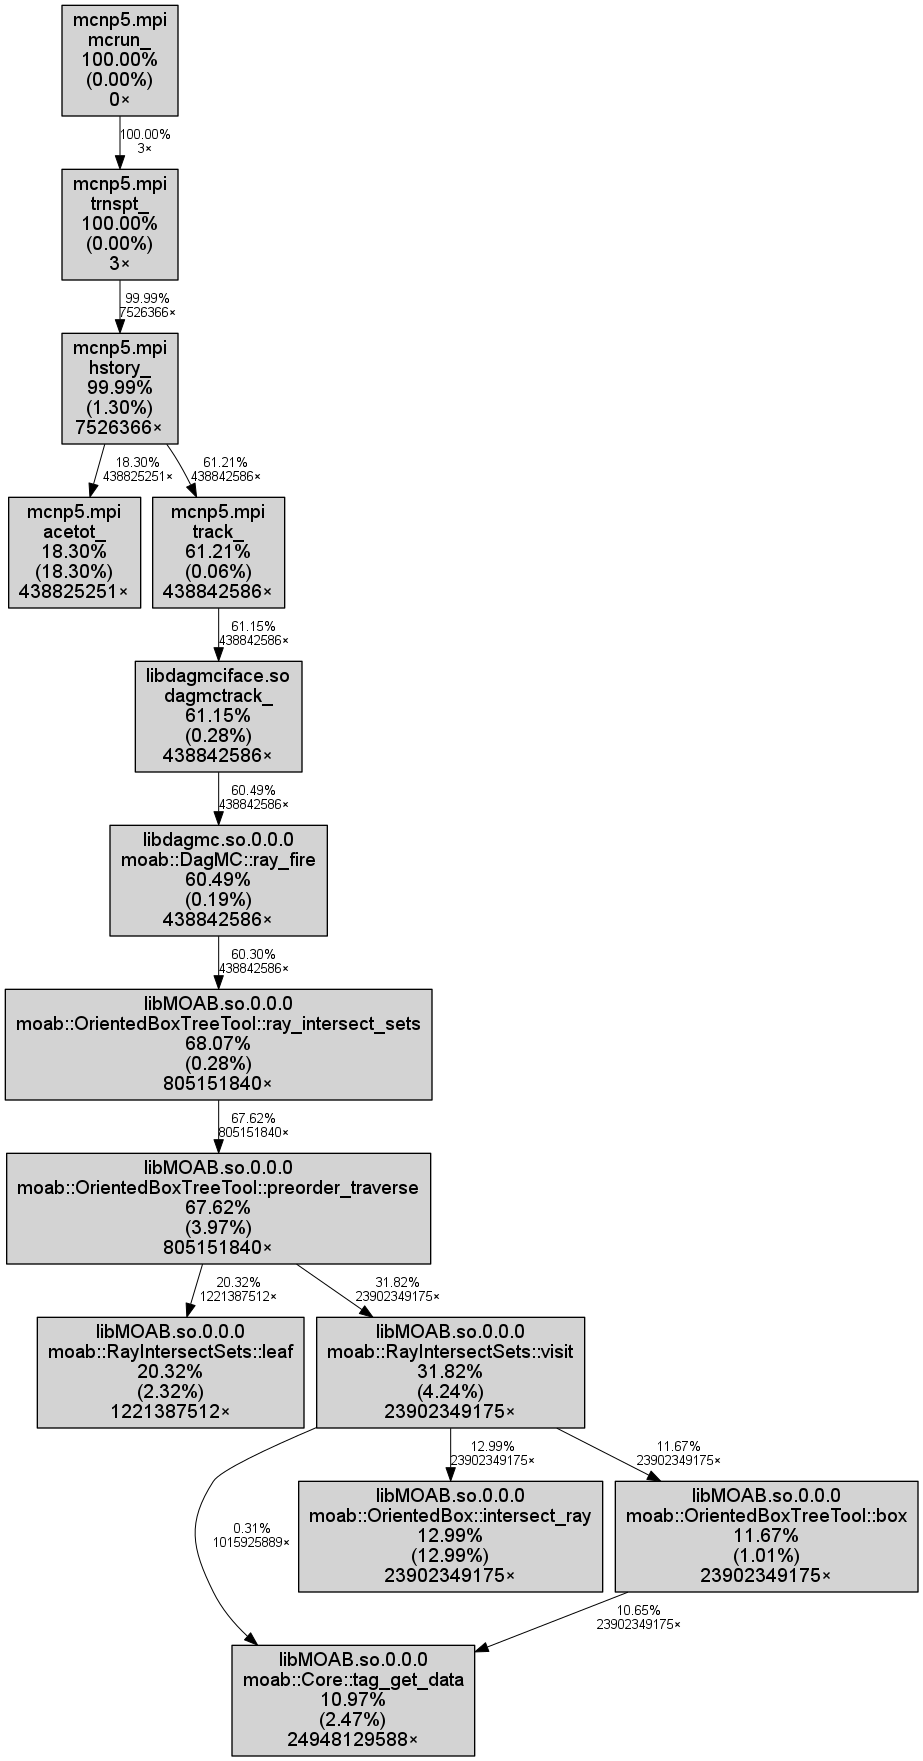
\includegraphics[scale=0.3]{dagmc_fng_cg_coarse.png}
\end{figure}

\begin{figure}[H]
  \centering
  \caption[Callgraph of a native MCNP simulation.]{Callgraph of native MCNP FNG run for \num{1E7} histories. Processes taking
    $<$10\% of the run time are filtered out in order to simplify the call
    graph.}
  \label{mcnp-fng-coarse}
  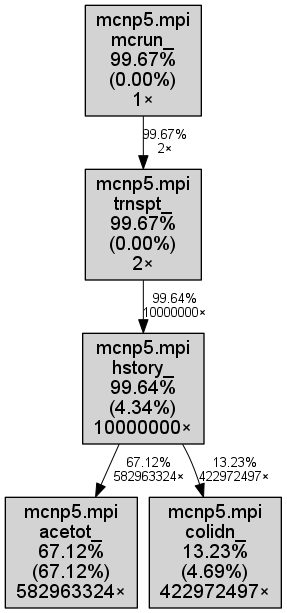
\includegraphics[scale=0.3]{native_fng_cg_coarse.png}
\end{figure}

The combination of the profiling results indicating how much time is spent in
tracking particles in DAGMC along with the difference in absolute simulation times
confirms that the performance bottleneck of DAGMC lies in its ability to quickly
satisfy the geometric queries of the underlying Monte Carlo code it is coupled
to. Looking more closely at the underlying calls in DAGMC, one can see that this
time is collectively spent in the DAGMC \textit{ray\_fire} method. Function names
like \textit{RayIntersectSets} and \textit{preorder\_traverse} indicate that
this time is spent in MOAB's database-oriented ray tracing implementation.

\section{Statement of Thesis}

The purpose of this dissertation is to improve the performance of CAD-based
Monte Carlo radiation transport in a manner that is widely accessible to
analysts. The result is a compilation of adaptive data structure construction,
data structure redesign, and alternative methods to reduce simulation times in
DAGMC.

A background and literature review of CAD-based transport methods and associated
acceleration techniques is provided in Chapter \ref{ch:background}. First, it
outlines required capabilities for particle tracking in Monte Carlo Radiation
Transport (MCRT). Next it describes 
commonly used geometry representations in MCRT codes followed by a description
of the CAD-based particle tracking systems of interest for this work. Lastly,
associated acceleration data structures and techniques which enable highly performant
computation of transport on CAD models are discussed.

Chapter \ref{ch:preconditioning} presents a novel acceleration method for
CAD-Based MCRT and its application for each of the relevant geometry query types
outlined in Chapter \ref{ch:background}. An analytic model is then described to
guide the application of this technique based on simple parameters of the problem geometry
and physics. Finally, results of this
method's application in both contrived and production models are discussed along
with limitations of the method and aforementioned analytic model.

The integration of nuclear engineering simulation with state-of-the-art
computer graphics tools is demonstrated in Chapter \ref{ch:simd_bvh}. Significant
improvements in performance are demonstrated in both test and production models
by adapting data structures discussed in Chapter \ref{ch:background} for optimal
efficiency on modern CPU architectures. Robustness limitations of the computer graphics
tools for engineering analysis are discussed, and extensions of these tools are
presented to address those limitations. Critical implementation details and
algorithmic adjustments of these
extensions are outlined, and performance comparisons are drawn in terms of the
raw query speed between all particle tracking implementations. Finally results,
of the extended, and robust, system are presented for several production models,
including several of the models used as an initial comparison in Chapter
\ref{ch:introduction}.

Chapter \ref{ch:high_valence} addresses a long-standing issue in CAD-based
MCRT. Performance degradation caused by problematic features of the CAD-based mesh geometry
are characterized using a contrived model for all ray tracing
implementations in Chapter \ref{ch:simd_bvh}. A solution using on-the-fly
detection and adaptation of this feature during construction of particle tracking
acceleration data structures is presented. Characterization of the performance
both with and without the adaptive construction
technique are presented and discussed. Finally, results of this technique as applied to the same set of
production models shown in Chapter \ref{ch:simd_bvh} are presented and discussed.

The conclusion statements in Chapter \ref{ch:conclusion} discuss the
contributions of this work to MCRT for CAD geometries, its broader impacts, and
possible future directions for various aspects of the work.

\newcommand{\geomQuery}[3] {
  \null %emptyline
  \textbf{\uppercase{#1}} 
  \begin{adjustwidth}{2.5em}{0pt}
      \begin{tabular}{p{8cm} p{2cm}}
    #3
    &
    \raisebox{-\totalheight}{\includegraphics[width=0.3\textwidth]{#2}}
  \end{tabular}
  \end{adjustwidth}
}

\chapter{Background}\label{ch:background}

\section{Monte Carlo Geometry Queries}\label{sec:mc-geom-queries}

A Monte Carlo geometry kernel must be able to robustly support the following
types of geometry queries

\geomQuery{Point Containment}{plc_query.eps}{
    Given a volume and particle location, determine if the point is inside,
    outside, or on the boundary of that volume.
}

\geomQuery{Next Surface}{dtb_query.eps}{
  Given a volume, particle location, and particle trajectory, determine the next
  surface of the volume that the particle intersects along with the distance to
  that intersection.
}

\geomQuery{Closest Surface}{ctl_query.eps}{
  Given a volume and particle location, determine the distance to to the nearest
  surface of the volume in any direction.
}

\geomQuery{Next Volume}{sc_query.eps}{
  Given a volume and surface, determine the adjacent volume on the other side of
  the surface.
}

\geomQuery{Surface Normal}{normal_query.eps}{
  Given a surface and particle location, determine the normal vector of the
  surface at a point closest to the particle's location.
}

\geomQuery{Measure}{measure_query.eps}{
    Given a volume or surface in the geometry, determine properties of that entity
  such as the volume or area.
}

\section{Analytic Geometry Representations}\label{sec:analytic_geometry}

This section contains a discussion of common analytic geometry  representations
which are often used as native representations of Monte Carlo geometry.

\subsection{Implicit Surfaces}\label{subsec:implicit_surfaces}

An implicit surface is a multivariate function defined over an $ R^3 $ domain as:

\begin{equation}
    \Omega(R^3)\rightarrow R
\end{equation}

Implicit surfaces are a rich and versatile representation of closed manifolds
used for modeling, simulation, and rendering. Implicit surfaces are defined
using the isocontour of a scalar function defined over all space unlike an
\textit{explicit} representation of a surface which defines the subset of space
which the boundary occupies. Intuitively it might seem wasteful for a definition
to be true for all space considering the relatively small amount of space the
object will occupy, however a number of powerful tools for geometric modeling
using these representations will be discussed in this section.

An isocontour of this function with the value, $v$, can be described as:

\begin{equation}
  \Omega(\vec{x}) - v  = 0 
\end{equation}

For simplicity, the boundary of an implicit surface is defined as the isocontour
for which $v=0$. As a result, any point inside of the surface will have a negative value
while any point outside of the surface will have a positive value.

Unlike their explicit counterparts, implicit representations allow complex
topologies of surfaces to be integrated into a single representation. This is in
part because the function is defined for all space. As a result they handle the
merging and separation of disparate volumes well. These properties allow for
straightforward representation of dynamics surfaces such as fluids, though this
is not of concern in the area of radiation transport. In practice, implicit
surfaces are often used to extract mesh representations of surfaces, re-sample
the model into some other proxy for the geometry, and render models via ray
tracing. Additionally, implicit surfaces can be used to generate triangle meshes
for rasterization or rendering on GPUs \cite{Sethian_1996} and can also be
constructed from arbitrary triangle meshes or point clouds
\cite{Sigg_2006}. Implicit surfaces are well-suited to these applications due to
the integrated geometric properties that can be quickly recovered from their
analytic forms.

Geometric information needed for visualization and simulation can be
readily recovered from implicit surface representations. For example, a common
operation in particle transport is the determination of its containment by a
volume in the model. A quick evaluation of the implicit function for this point
will indicate its containment by the sign of the function.
%% Such a process is more complex in the case of an explicit or discretized
%% representation. Typically this involves casting a ray through the model and
%% counting up the intersections or relying on the orientation of triangle normals
%% to indicate an entering or exiting intersection. The oddness or eveness of the
%% number of crossings will then determine the points containment.
Additionally, the distance to nearest intersection with the surface from any
point in space can quickly be determined via the definition of a signed distance
function, $d(\vec{x})$, formally defined as:

\begin{align}
  & d(\vec{x}) = min(|\vec{x} - \vec{x_{I}}|) \\
  & \Omega(\vec(x))  \,s.t.  \,|\Omega(\vec{x})| = d(\vec(x)) 
\end{align}

\begin{align}
  d \, &- \, signed \, distance \, function \\
  \vec{x_{I}} \, &- \,nearest \, boundary \,intersection
\end{align}

\noindent
Meaning that implicit surface functions can be modified to meet the three
requirements of a signed distance function:

\begin{figure}[H]
  \begin{center}
    \begin{minipage}{.8\textwidth}
      \begin{itemize}
      \item $ \Omega(\vec{x}) = d(\vec{x}) = 0 $ for all $x$ on the surface boundary
      \item $ \Omega(\vec{x}) = -d(\vec{x}) $ for all $x$ inside the surface boundary
      \item $ \Omega(\vec{x}) = d(\vec{x}) $ for all $x$ outside the surface boundary
      \end{itemize}
    \end{minipage}
  \end{center}
\end{figure}

Implicit surfaces are often used in time-dependent simulations due to their
natural extension into a fourth dimension ($ \Omega(\vec{x},t) - v  = 0 $) and
thus their support for moving boundaries and changing topologies. Dynamic
geometries are not yet of concern for CAD-based Monte Carlo work, but
specialized forms of implicit surfaces are used as native geometry
representations in most Monte Carlo simulation codes.

\subsection{Constructive Solid Geometry}\label{subsec:csg}

Native Monte Carlo geometries are commonly formed from a standard set of
well-behaved implicit surfaces known as general quadratics. These surfaces are
then combined through Boolean operations to form more complex objects as shown
in Figure \ref{fig:csg_ex}.

\begin{figure}[h]
  \centering
  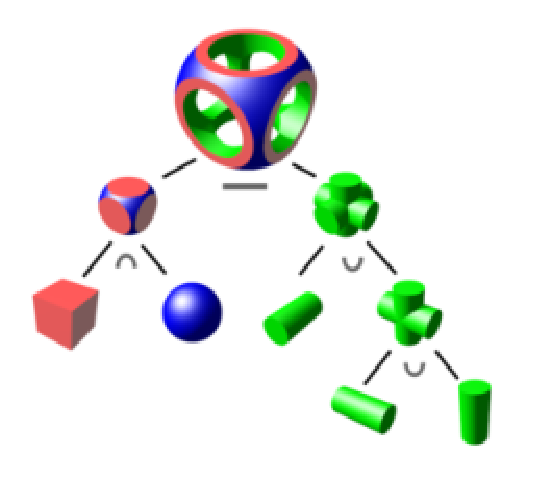
\includegraphics{csg_ex.eps}
  \caption{An example of how CSG volumes are created using Boolean combinations
    of objects. The union of the three orthogonal cylinders is
    subtracted from the intersection of the box and sphere on the left to form
    the final volume at the top of the figure.}
  \label{fig:csg_ex}
\end{figure}

It is possible to construct complex geometries using CSG, but, as mentioned in
the introduction, the interface for this work is typically text-based, making
defining complex volumes a tedious and time-consuming task. Detecting
problems with the geometry definition is straightforward for the same reason
that particles can be robustly tracked through the geometry - the analytic
description of the surfaces. Fixing undefined regions of the geometry or
detecting invalid volume definitions is more difficult however.

The detection of intersections and particle containment queries in CSG
geometries is computationally inexpensive for volume definitions constructed
from a small number of surfaces, but, due to the logical combinations of
surfaces used to create volumes, the number of evaluations necessary to satisfy
these queries is linear with the number of surfaces in the definition. For
sufficiently large and complex models, it is not uncommon for volumes with many
surfaces to be artificially separated by planes to create two volumes with fewer
surfaces in their definition.

Visualization of CSG models is also somewhat limited. Because native formats for
CSG differ greatly between each Monte Carlo code, each typically provides its
own geometry visualization tools. These tools are typically restricted to 2D
images of the model representing a user-specified slice through the
geometry. Other tools such as MCAM \cite{Liu_2005} and McCad
\cite{Tsigetamirat_2008} allow for interactive visualization and repair of CSG
models, but these systems often require simplifications of the true model in
translation.

\subsection{CAD Geometry}

CAD systems allow for efficient and accurate representation of geometrically
complex domains. Models can be created using interactive visualization tools
represented in 3D space with a rich tool set for volume and surface
creation. These creation and modification tools along with the immediate visual
verification of a user's work reduces human error in model generation and design
iteration.

\begin{figure}[H]
  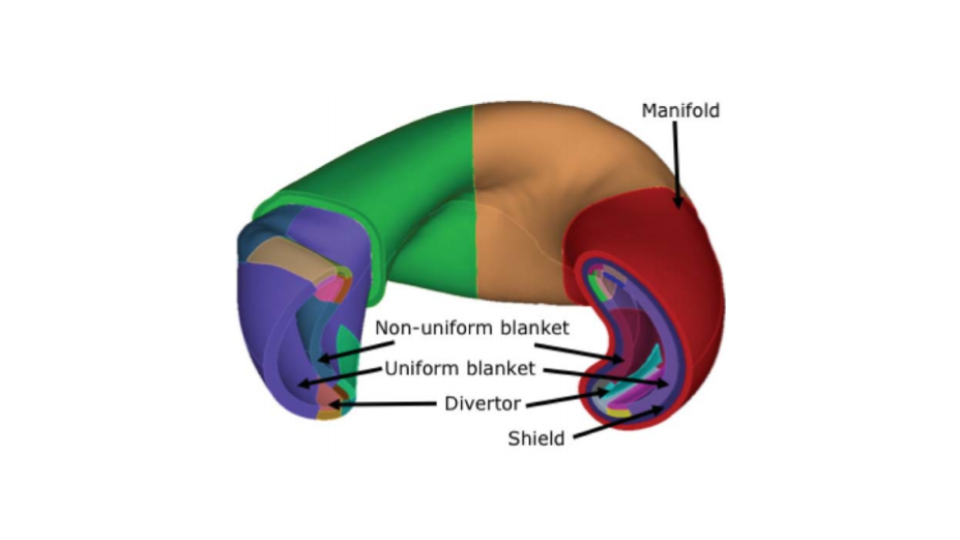
\includegraphics[scale=0.5, trim={100, 0, 0, 0}]{cad_stellarator.png}
  \caption{The vacuum vessel of a stellarator CAD model.}
  \label{fig:cad_stellarator}
\end{figure}

In addition to reducing human error, CAD models provide a common domain for
analysis in other engineering domains such as fluid dynamics, heat transfer, and
structural engineering. This shared domain creates a common domain for
parametric studies, iterative design, and coupled physics simulations. CAD
engines also provide the ability to represent free-form or higher-order
surface. The use of representations like splines and subdivision surfaces allow
for more accurate representation of complex forms which would be impossible to
accurately represent using CSG.

\begin{figure}[h]
  \centering
  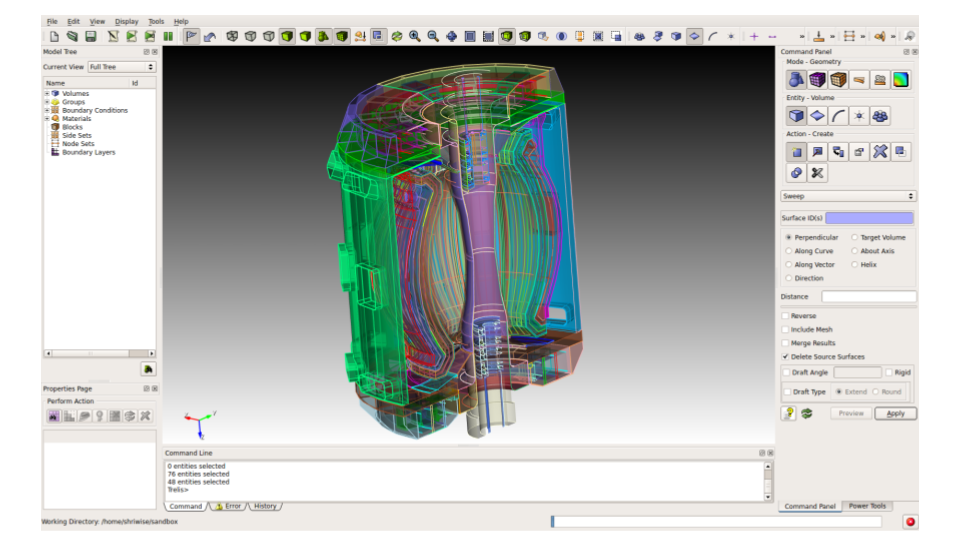
\includegraphics[scale=0.4]{cad_fnsf.png}
  \caption{The Fusion Neutron Science Facility (FNSF) model in the CUBIT \cite{Blacker_1994}
    CAD system.}
  \label{fig:cad_fnsf}
\end{figure}

\subsection{Monte Carlo Radiation Transport on CAD Geometry}

The Direct Accelerated Geometry Monte Carlo (DAGMC) software toolkit enables
Monte Carlo radiation transport directly on CAD geometries
\cite{Tautges_2009}. DAGMC was developed at the University of Wisconsin -
Madison and has been coupled with many Monte Carlo codes. DAGMC relies on
Cubit\cite{Blacker_1994} (and its commercial counterpart, Trelis) for CAD
modeling.

More specifically, DAGMC provides robust particle tracking for the underlying
physics kernels of various Monte Carlo codes. It accomplishes this by
discretizing CAD surfaces into sets of triangles. Volumes are then defined by
any triangles which represent bounding surfaces of a given volume. This surface
mesh and the geometric relationships between the mesh entities are stored in the
Mesh Oriented dAtaBase (MOAB) \cite{Tautges_2004}. These relationships, which
preserve the geometric topology, are stored in a hierarchical structure within
MOAB, relating volumes to their surfaces, surfaces to curves, and curves to
vertices.

It is important that geometric relationships of the mesh are maintained to
accelerate certain geometric queries on the surface mesh. For example,
\textit{Next Volume} queries are accelerated by using these relationships to
directly determine which volume a particle is passing into upon crossing a
surface. In CSG, a surface crossing can require a series of point containment
checks for each volume to determine new volume and media. Other queries become
more complicated, however, due to the sheer number of triangles needed to
properly define volumes with detailed features.

\textit{Next Surface} and \textit{Closest to Location} geometry queries, for
example, can be computationally expensive for volumes composed of hundreds of
thousands or even millions of triangles. A convenient way to think about
performing geometric queries on triangulated surfaces or volumes is to consider
an equivalent CSG representation constructed using a planar surface in place of
each triangle in the DAGMC model. The structure imposed by the Boolean
combinations used to define such volumes require that each surface be checked
for an intersection with the particle trajectory. The nearest of these
intersections can then be used to determine the location of surface crossings.

The problem of finding a surface intersection for a given particle location and
trajectory with a set of geometric primitives is a well-researched problem in
the field of ray tracing. In this field, data structures designed to accelerate
the location of the nearest ray intersection are used to render animations and
images in real time.

\section{Ray Tracing Acceleration Data Structures}

Acceleration data structures for ray tracing are designed to rapidly narrow the
search for an intersection in 3D virtual space given a starting position and
direction also known as a ray. This is accomplished by partitioning the space
and associating geometric primitives, usually triangles, with that bounding
partition. A search is performed by checking for an intersection with the
bounding partition. If the ray does not intersect with the partition, then the
set of primitives associated with that partition can be removed from the
search. If the ray does intersect with the partition, then the set of associated
primitives must be checked for intersection. Because a single separation into
two spatial partitions is often insufficient to increase search efficiency, this
partitioning process is performed recursively. The result is a tree, or
hierarchy, structure in which partitions at the top of tree are associated other
partitions, known as child nodes, rather than primitives. Partitions at the end,
or bottom, of the tree are associated with geometric primitives representing the
volume boundary.

The search for a ray intersection then becomes a traversal of the tree in which
the children of the root node are checked for intersection. If an intersection
is found with one or both of the nodes, then the corresponding child nodes are
checked for intersection as well. This process is repeated until leaf nodes are
reached at which point primitives are checked for intersection. Any primitives
underneath a node with which the ray does not intersect can immediately be
rejected as a possibility for a hit. This allows many primitives to rapidly be
removed from the search and limit the number of true intersections to a small
number compared to checking each primitive individually. This technique reduces
the algorithmic complexity of the search from a brute force, or linear
$O(log(N_{triangles})$ , search to a logarithmic $O(\, log(N_{primitives}))$
search.

\subsection{Partition Splitting Heuristics}

There are two critical components that go into the creation of spatial
partitions in ray tracing hierarchies. The first is the selection of a candidate
splitting plane which is used to separate entities into one partition or
another. The second is the evaluation of the ``cost'' of that split should it be
used. This cost is representative of the comparison between a division of the
node for several candidate split planes and forming a leaf from the current
node.  Because there is no way to know exactly how expensive or inexpensive a
split will be for the particular simulation at hand, heuristics are used to
evaluate this cost and determine the optimal splitting plane using limited
information about the local nodes in the tree. More specifically, this
information is typically limited to the number of primitives and bounds of the
parent partition and resulting child partitions.

An infinite number of planes could be tested to find the optimal plane for
dividing the entities between the two child volumes, but even if one were to
encounter such a splitting plane, it can be difficult to identify the plane as
such without more knowledge about the final tree structure. As a result, a
limited set of planes is tested for the best split based on a set of assumptions
about the problem at hand and the heuristics being used to evaluate split
costs. The most common method for split plane candidates is median plane
splitting in which a bounding volume is split in half for each axes of the
current bounding volume. The splitting planes are then evaluated and the split
with the lowest cost is selected. Other methods for plane selection exist, but
will not be discussed in this work as it is more focused on traversal performance.

Two heuristics will be discussed here - the Entity Ratio Heuristic (ERH) and the
Surface Area Heuristic (SAH). The ERH uses the resulting number of
primitives in each child node to determine the cost of a split. The philosophy
behind this heuristic is to maintain the expected $O(log(N_{triangles})$ cost of
a ray traversal by ensuring that primitives are split as evenly as possible from
parent to child node. A form of this heuristic is presented in
Eq. \ref{eq:ERH}. The ERH cost is unitless and bounded by zero and
one. This makes it possible to set both an upper and lower bound on the
unacceptable cost and a ``good enough'' cost.

\begin{figure}[H]
\begin{equation}
\label{eq:ERH}
 C = \frac{|P_{R}-P_{L}|}{(P_{R} + P_{L})} 
\end{equation}
  \begin{align*}
    C - & \,final \, cost \, evaluation \\
    P_{L} - & \, primitives\, contained\, by\, the\, left\, child  \\
    P_{R} - & \, primitives\, contained\, by\, the\, right\, child \\
  \end{align*}
  \caption{An example of the entity ratio calculation for a binary tree.}
  \label{fig:ERH}
\end{figure}

The SAH applies spatial information as well as division of primitives to the
cost evaluation. Its full form is found in Equation \ref{eq:SAH}. The SAH uses
the surface area of candidate child partitions relative to the parent
partition's surface area as an approximation for the probability that the child
will be visited after the parent volume. This evaluation relies on the
assumption that rays in the problem are globally isotropic. The explicit form of
the surface area heuristic was introduced in 1987 by Goldsmith and Salmon
\cite{Goldsmith_1987} and later formalized by MacDonald and Booth in 1990
\cite{MacDonald_1990}.

\begin{figure}[H]
  \begin{equation}
    C =  C_{t} + \frac{SA_{L}}{SA_{P}} |P_{L}|C_{i} +  \frac{SA_{R}}{SA_{P}} |P_{R}|C_{i}
    \label{eq:SAH}
  \end{equation}
  \begin{align*}
    C_{t} - & \,cost\, of\, traversal\, to\, child\, nodes \\
    C_{i} - & \, cost\, of\, primitive\, intersection\, check\, \\
    SA_{L} - &  \,surface\, area\, of\, left\, child \\
    P_{L} - & \, primitives\, contained\, by\, the\, left\, child  \\
    SA_{R} - & \, surface\, area\, of\, right\, child \\
    P_{R} - & \, primitives\, contained\, by\, the\, right\, child \\
    SA_{P} - & \, parent\, bounding\, volume \\
  \end{align*}
  \caption{A form of the surface area heuristic for a binary tree.}
  \label{fig:SAH}
\end{figure}

For the general case, ERH has not proved to be as effective as the SAH, but it
has proven to be a useful tool in correcting the surface area heuristic for
triangle mesh features of a specific type. This scenario will be discussed further
in Chapter \ref{ch:high_valence}.

\subsection{KD-Trees}
\label{subsec:kd-trees}
The KD-Tree or multidimensional binary search tree was originally developed as
an acceleration data structure for querying records in databases and has since
found use in other applications including speech recognition, global information
systems, and ray tracing \cite{Bentley_1975}. KD-Trees operate by using single
values to represent divisions in a dimension of the problem space. A different
dimension is split in each level of the tree, and the process is recursively
repeated until a sufficiently small number of records or entities exist within
the resulting partitions of a split, resulting in leaf nodes of the tree.

This data structure is commonly applied to virtual 3D space for ray intersection
queries. A different dimension of space is split in each level of the tree just
as is done in the context of an arbitrary database with different indices of
data. The values used for separation of entities in the tree now represent a
coordinate of a plane in that dimension; entities are then sorted to either side
of that dimension to perform a split. First, the problem space is divided evenly
in the x dimension. The two child partitions are then divided along the y axis
and the resulting children of this division are subdivided along the z
axis. Divisions are typically done in such a way that the space of the current
candidate is bisected, however it is possible that by doing this primitive
entities are divided by the plane as well. There are a couple of ways in which
this problem is handled. The first is to simply reference any intersected
primitives in both of the subdivisions. This means that some primitives may be
checked for intersection more than once, but requires no changes to the original
model. The other solution is to divide the primitive entities using the
partition plane.  This solution requires alterations to the model which may be
undesirable under certain conditions and violates the description of the KD-Tree
as a pure querying structure by making modifications to the existing model.

\begin{figure}[H]
  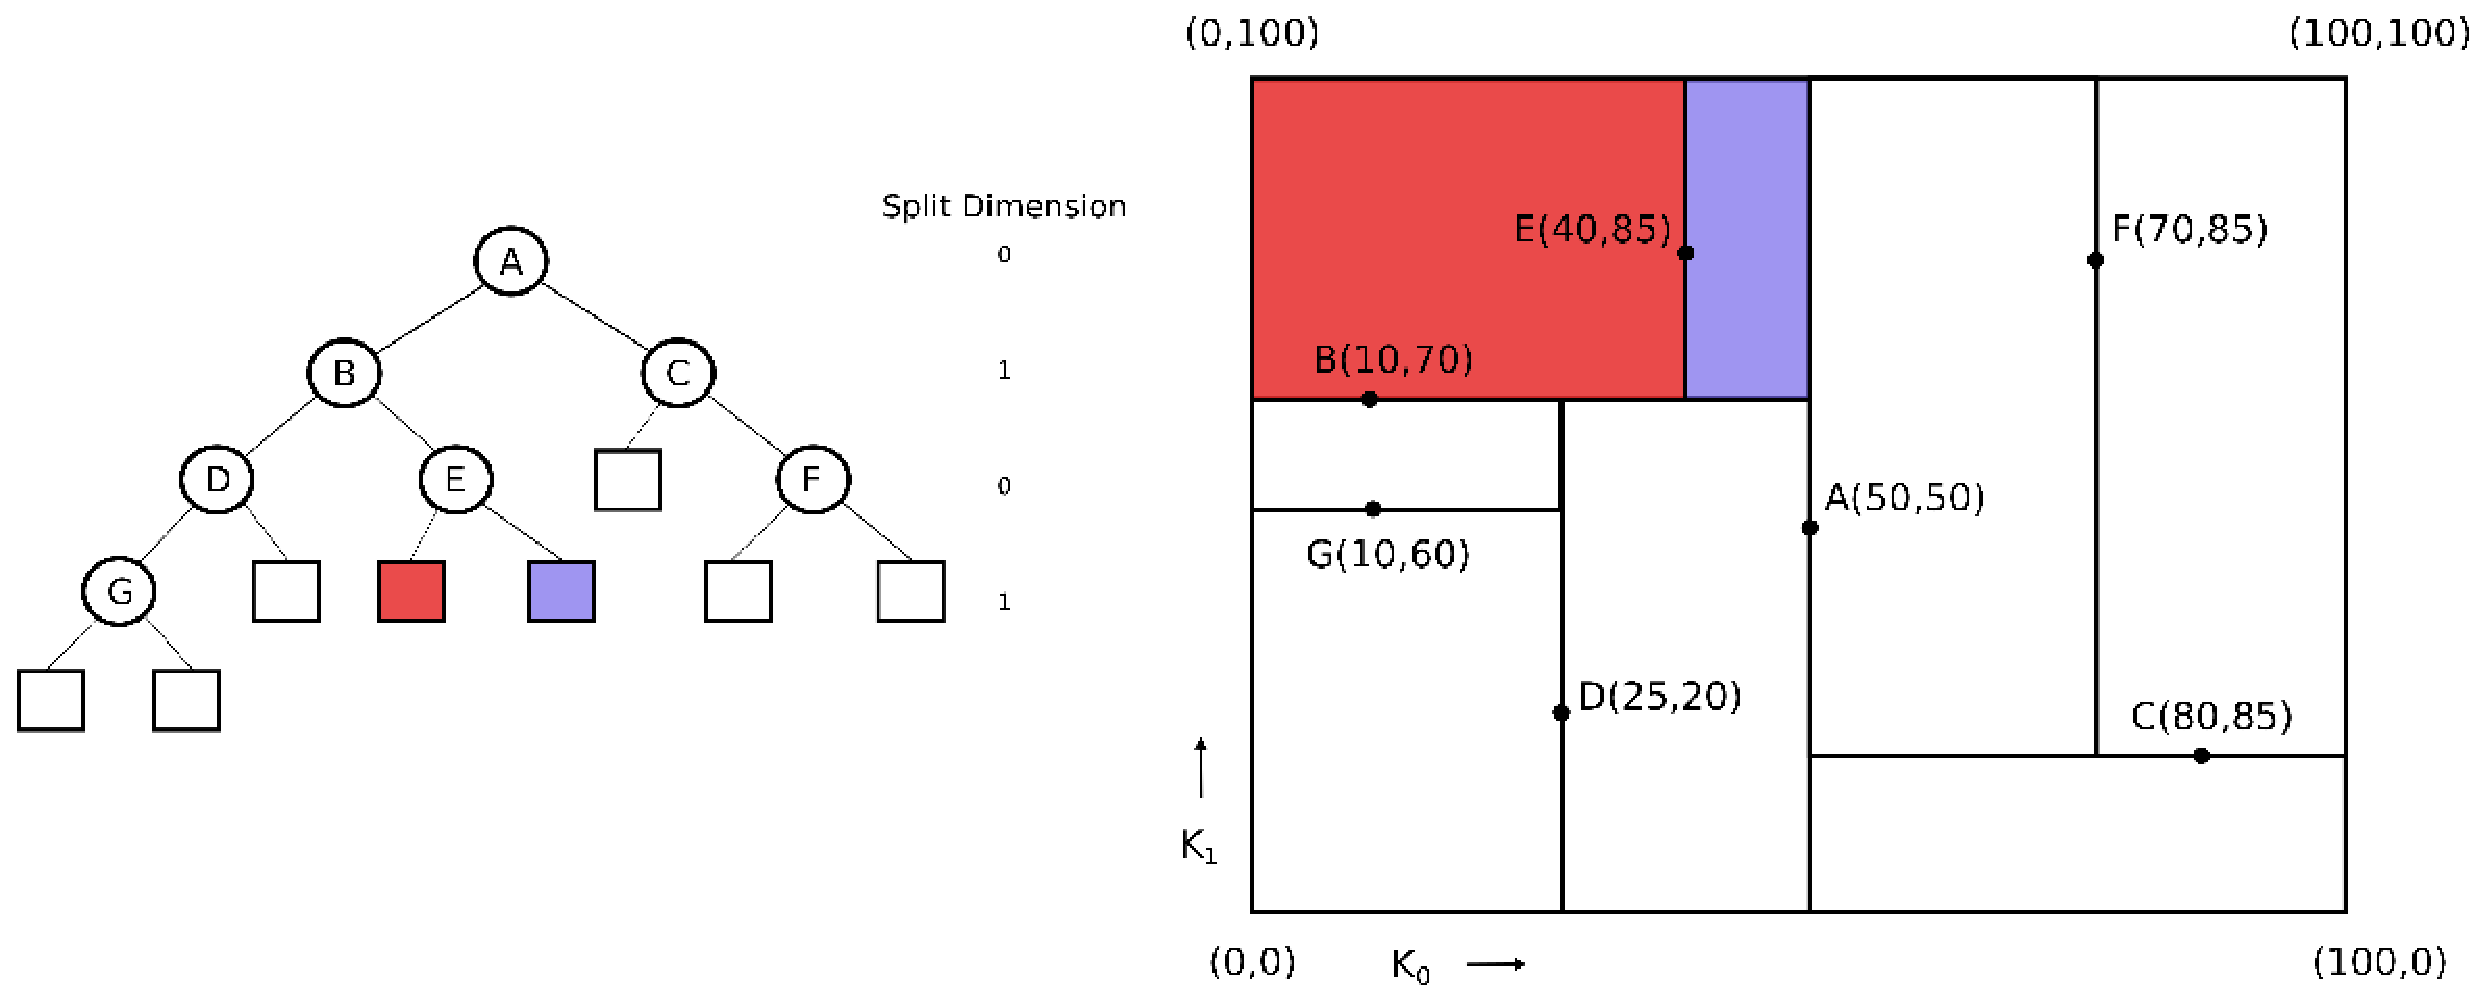
\includegraphics[scale=0.25]{2d_kd_eg.eps}
  \caption{Depiction of a two dimensional KD-Tree example adapted from Bently
    et. al. \cite{Bentley_1975}. Left: Graph representation of the
    KD-Tree. HISON's are right children. LOSON's are left children. Boxes are
    leaf nodes. Right: Two dimensional space partitioned in the graph. Boxes represent
    the range of their respective sub-tree.}
  \label{fig:2D_kd_tree}
\end{figure}

KD-Trees are able to perform highly efficient due to traversal schemes developed
based on the inherent quality of KD-Trees' non-overlapping sibling nodes. As a
KD-Tree is being constructed, an ever-shrinking bounding box is being defined as
one moves deeper into the tree. At the leaves of a KD-Tree, a well-resolved
bounding box can be conceptualized using the coordinates of the last six
splitting planes visited. The conceptual construction of this box is one way to
move from node to node in a more efficient way than a more standard depth-first
approach used in tree traversal. The partitions whose planes are used to
construct this conceptual box can be linked to the current partition in order
maintain a spatially localized search within the hierarchy. These links are
referred to as neighbor links and, as shown by Samet et. al.\cite{Samet_1989},
can be used to significantly reduce traversal costs in the KD-Tree. During
traversal if a leaf is visited its neighbor links can be used to direct the
query to either the next adjacent leaf or a nearby interior node in the tree
thus avoiding a depth-first style traversal in which the next step upon visiting
a leaf node is to return to the root node of the tree and continue. These
neighbor links take advantage of the idea that if a leaf node is visited, but
the desired intersection is not found, then it is likely that the desired
intersection is close to the current leaf location. In this way, one can avoid
large amounts of unnecessary shallow and mid-level tree traversal steps.

KD-Trees are frequently cited as being able to provide the best ray tracing
performance to date \cite{Ernst_2007,Hurley_2002,Havran_2000}. In particular,
KD-Trees are noted as being better equipped to handle models with highly varying
triangle sizes/densities. In practice, KD-Trees tend to be very deep and can
consume relatively high amounts of memory compared to other acceleration data
structures, however. 

\subsubsection{Bounding Volume Hierarchies}%%Status: Done%%
\label{subsec:BVH}
The initial concept of using the bounding volume construct as a pre-check for
ray-intersection with CSG objects was introduced by Weghorst in 1984
\cite{Weghorst_1984}. Weghorst explored the possibility of using bounding
spheres and bounding boxes to contain geometric objects. This work also went so
far as to create a hierarchy out of the object-based bounding volumes, noting the
importance of hierarchically joining bounding volumes near to each other in space
so as not to have parent volumes containing large amounts of empty space between them.

\begin{figure}[H]
  \centering
  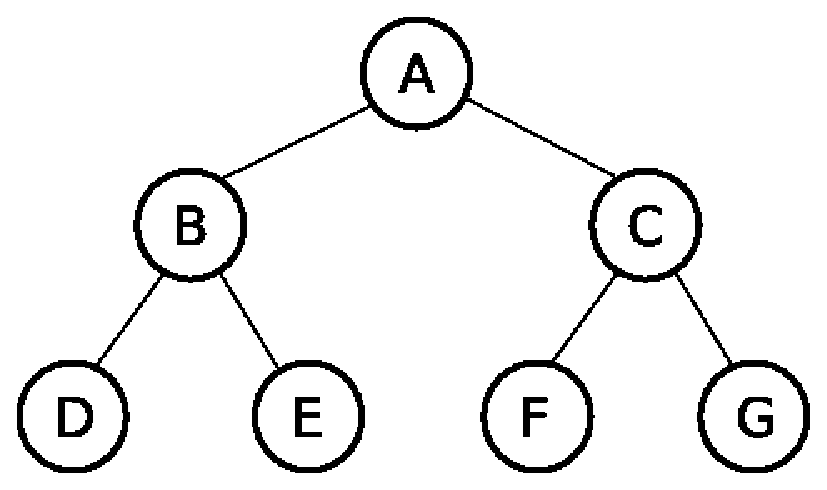
\includegraphics[scale=0.3]{binary_graph.eps}
  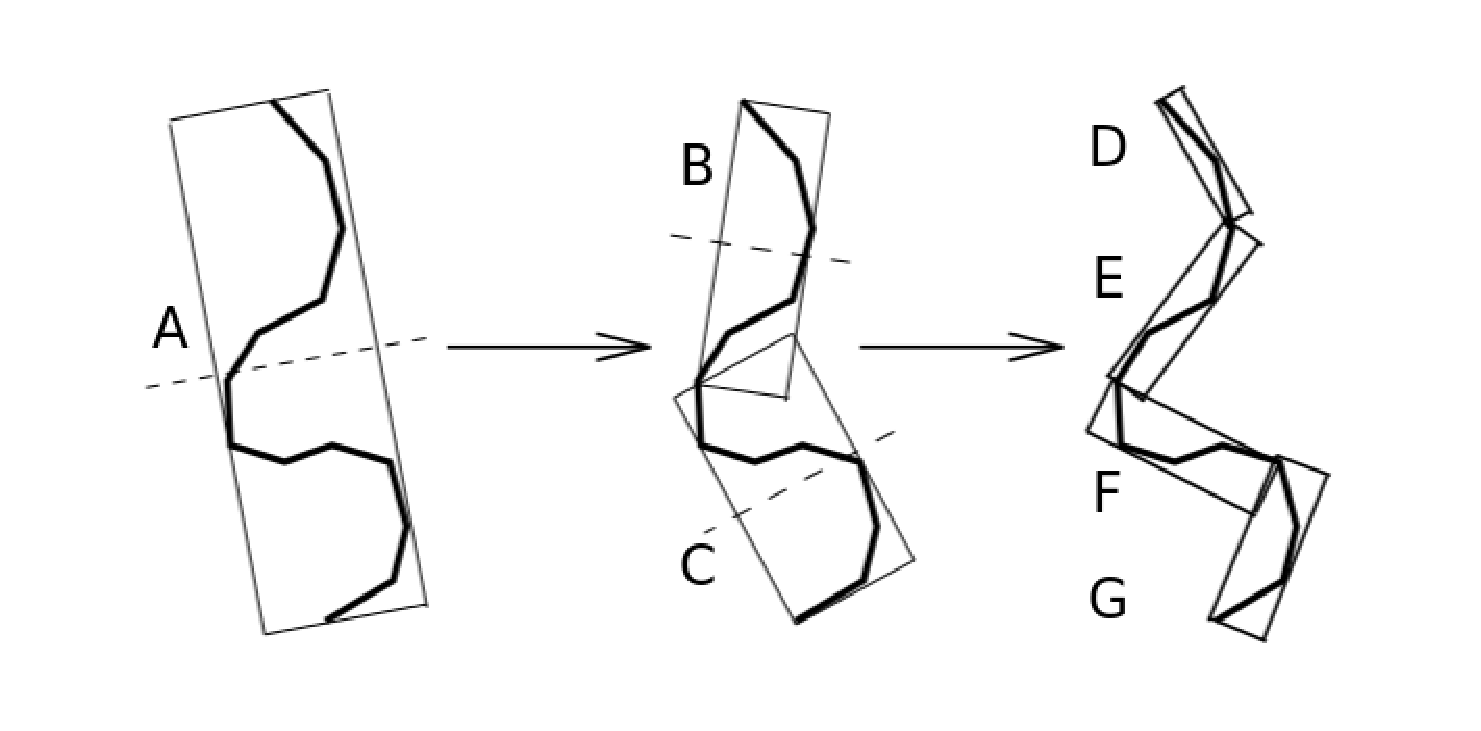
\includegraphics[scale=0.3, trim = 0 50 0 0 ]{bvh_2d_ex.eps}
  \caption{Depiction of a two dimensional BVH example adapted from Gottschalk 1996 \cite{Gottschalk_1996}}
  \label{fig:2D_bvh}
\end{figure}

In Weghorst's exploration of sphere and box bounding volumes it was found that
while spherical bounding volumes are not as computationally expensive to check
for ray intersections than bounding boxes because the latter generally provide a
tighter fit to the objects they contain. This decreases the chance of wasted
ray-volume intersection checks for rays which intersect the bounding volume, but
not the object it contains. When considering the application of bounding volumes
to a discretized analytic surface represented by a triangle mesh, this becomes
 more important as BVH's become deeper and more ray-volume intersection checks are performed to
reach leaf nodes. Even applied to analytic objects, this effect was reflected
in the results of Weghorts's work strongly enough to show that bounding boxes
provided better performance in accelerating the ray intersection process than
bounding spheres.

Two forms of BVH's are commonly applied in ray tracing problems: Axis-Aligned
Bounding Boxes (AABBs) and Oriented Bounding Boxes (OBBs). AABBs are boxes whose
orientation is restricted such that their faces are parallel to the global
planes of the problem space. Given a set of points to contain, tightly fitting
axis aligned boxes are straightforward to construct. Their simple representation
results in a relatively low memory footprint and straightforward, yet robust,
ray-intersection tests. Unlike AABBs, the faces of OBBs are allowed take any
orientation relative to the global axes in order to enclose their set of
primitives as tightly as possible. Several robust methods for determining the
orientation of a box for best fit to a set of primitives have been developed
\cite{Gottschalk_1996,ORourke_1985}. OBBs are better for avoiding superfluous
ray-box intersections that might otherwise occur for an AABB. They also more
quickly conform to the full set of enclosed primitives as the boxes are
recursively divided. By orienting their axes with the local set of primitives
they are bounding, candidate splitting planes, usually selected in the reference
frame of the parent node's oriented axes, are more effective at separating
primitive entities and reaching leaf conditions quickly. This leads to more
shallow hierarchies making the worst-case number of intersection tests lower
than for an AABB hierarchy on average. While a shallow hierarchy might indicate
a smaller memory footprint, OBBs require one to store some extra information
about their orientation relative to the global axes making this assumption
difficult to consistently prove.

One disadvantage of using OBBs is that the ray-box intersection check requires
an extra step in transformation of the ray to the oriented axes of the box in
question. The information needed for transformation of the ray basis must be
applied to the ray before the box intersection can continue as it would for an
axis aligned box. Thus, for a given ray query, an OBB hierarchy may have fewer
intersection checks to perform than an AABB hierarchy, but the intersection
checks are inherently more expensive than in the case of OBBs. In practice,
AABBs are commonly used in BVH's for their simplicity of implementation and
well-researched ray intersection algorithms. Other reasons for this preference
will be discussed later in Section \ref{subsec:arch}.

There are multiple approaches to constructing a BVH given a set
of geometric primitives, but only ``top-down'' approaches will be discussed
here. A top-down approach begins with the construction of a single bounding
volume enclosing all primitives which will be part of the tree. At this point,
child boxes of this root volume are created by selecting a splitting plane for
the box which divides the primitives contained by the current bounding volume
into two subsets. This process is then repeated until leaf conditions are
met. The selection of candidate splitting planes and the selection of a final
plane for splitting based on its estimated worth can greatly affect the
performance of the data structure.

One difficulty that BVH's of any type face is that of overlapping sibling
bounding volumes. Overlapping sibling volumes can cause additional box
intersection checks in a similar manner to loosely fitting bounding volumes. If
a ray enters a region of overlapping sibling volumes, this causes the children
of both boxes to be checked despite the fact that the ray will eventually only
intersect with primitives contained by only one of the boxes. Overlaps are
difficult to avoid, however, due to the reality that volumes are required to
contain discrete elements for robustness, not just a section of the virtual
space. Simply put, if the splitting plane of a bounding volume goes through one
of the geometric primitives, there will be an overlap in the resulting child
volumes. Overlaps of sibling AABBs are typically limited to the size of perhaps
one or two geometric primitives, but this inefficiency can be exacerbated by the
structure of triangulated objects the BVH's are being formed around. One such
feature which will be addressed in Chapter \ref{ch:high_valence}.

The spatial BVH variant (SBVH) was introduced by Stich et. al. in 2009
\cite{Stich_2009} with an additional complexity to the node splitting step. As
candidate split planes are considered, triangles (or
geometric primitives) are duplicated and contained in both resulting nodes. This grants much
more freedom when considering how a node should be partitioned. The relatively simple application of this
method is performed by considering both splits in which triangle duplication is
prohibited and splits in which it is allowed. In the scenario for which triangle
duplication is prohibited, the set of candidate planes is equivalent to that of
a standard BVH building algorithm. Stich applies the surface area heuristic for
the purpose of his publication. In the case where reference duplication is
allowed, the search for a splitting plane is much more open - as previously
mentioned. In fact, the search becomes fundamentally aligned with the search for
a spatial split as might be found in a KD-Tree implementation. The optimal
splitting plane is then selected via a comparison of the SAH cost for all
candidate split planes - spatial or ``traditional''. Secondary heuristics are used
to limit reference splitting in an effort properly manage the data structure's
memory footprint. The result of the SBVH is a hierarchy which can be traversed
just like any other BVH but with significantly reduced sibling volume
overlaps. The SBVH results consistently show significant improvement over other
methods, ranging anywhere from (20-100\%) \cite{Stich_2009}.

In summary, bounding volume hierarcies are favoered in the field of ray tracing
for their lower memory footprints and well-developed parallel building
schemes. These features are of great import for systems with limited memory,
such as GPUs, and applications with intent for realtime viewing or
interaction. These data structures are particularly performant for \textit{Next
  Surface} intersections and are currently the most commonly employed
acceleration data structure for ray tracing. They are relatively simple to
implement for the performance they are able to provide and have a smaller
footprint relative to most other ray tracing acceleration data structures,
making them attracitve to memory-limited environments such as GPUs.

\subsubsection{Octrees}%%Status:Done%%
\label{subsec:octree}

Octrees are a partitioning scheme in which cuboid bounding boxes known, also
known as voxels, are used to partition the 3D problem space into the 8 quadrants
defined by the global axes and extents of the parent voxel. These 8 voxels are
then linked as children of the parent voxel. This process is repeated
recursively until leaf conditions are met in which a sufficiently small number
of primitives is contained within the current voxel.

This spatial subdivision technique is commonly used to efficiently index
data in 3-D space \cite{Glassner_1989}. Octrees are somewhat like KD-trees in
that their divisions are spatial, their partitions contain no overlaps, and the
placement of entities in nodes occurs in a similar manner to that of KD-trees,
but each node is represented by a closed bounding volume as in a BVH.

Octrees can consume a large amount of memory relative to the data
structures previously discussed in this chapter. It is often possible that
voxels may be completely devoid of underlying entities. There are typically many
voxels containing no primitive references but may be required to exist as part
of the data structure. This results in many voxels being stored in memory which
aren't useful other than to verify that the space they contain is
empty. Additionally, geometric primitives may be referenced multiple times if
they intersect multiple nodes thus increasing the required memory storage with
the same consequence as seen in KD-Tree traversl with the possibility of a
primitive being checked more than once upon traversal. The memory footprint is
mostly of concern in applications for visualization on GPUs - though specialized methods for Octree applications on these architectures do exist.

\begin{figure}[H]
  \centering
  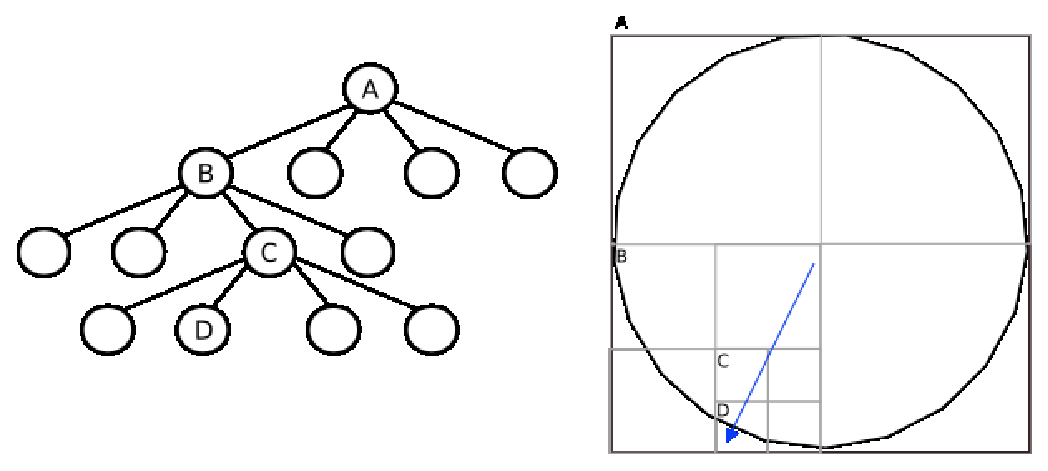
\includegraphics[scale=0.65]{octree_2d_ex.eps}
  \caption{Depiction of a two dimensional Octree example of a top-down ray fire traversal for a simple geometric object.}
  \label{fig:2D_octree}
\end{figure}

One advantage of octrees is the regular nature of the partitions. The value of a
node in hierarchies such as these (or in the BVH for that matter) lies in its
ability to remove candidate space from the query, yet a voxel can only
accomplish this if rays strike the voxel. The result is that one measure of a
voxel's value can be described by the ratio of its probability of an
intersection check to the space it will exclude from the query search or its
volume. In a problem with a uniform ray distribution, the probablity of a ray to
intersect a given voxel can be related to a voxel's surface area as seen in the
SAH. Thus cubic voxels have the most favorable ratio possible based on their
geometry. The uniformity of voxel properties provide a predictable nature of the
octree which is advantageous when traversing the data structure as well.

The predictable size and location of any given node in the tree determined from
the root node properties also provides a fast lookup of the deepest node in the
tree containing a point in space. This is helpful in providing a starting point
for ray traversal which is deeper than the root node, allowing one to
potentially avoid some traversal steps in the shallow levels of the
tree. Additionally, octrees have non-overlapping nodes which allows for
efficient traversal schemes similar to the neighbor linked traversal done in
KD-trees. These traversals are conceptually similar to that of the KD-tree's but
typically employ some form of Morton encoding to determine which node in the
octree the ray should visit next \cite{Revelles_2000}. Other traversal
techniques allow the octree to avoid creating and traversing nodes containing
empty space which can significantly reduce its memory footprint in cases where
internal nodes of the tree aren't required to define some spatial dataset as
mentioned above \cite{Samet_1989}. These methods are often applied in GPU
environments due to the limited memory available there. Octrees are often used
to store spatial data fields as well and naturally provide a higher resolution
of the field near boundaries of volume as the voxels become smaller in that
region which can be seen in Figure \ref{fig:2D_octree}.

As mentioned above, octrees are known for having large memory footprints
compared to other acceleration data structures, but they can also be used
advantageously for a combined purpose if a problem requires the storage of one
or more well-resolved data fields near volume boundaries as well as the
capability for ray tracing.

\subsection{Architecture Based Acceleration}%%Status: Pending%%
\label{subsec:arch}

This section will focus on the advantages of vectorization implementations or
Single Instruction Multiple Data (SIMD) programming in the field of ray
tracing. When considering the problem of parallelism in computing, programmers
focus on one of two areas: \textit{functional parallelism} or \textit{data
  parallelism}. Functional parallelism describes the method of performing
multiple operations in parallel on many processors while data parllelism
describes operation on multiple data sets at the same time on a single
processor. SIMD is a form of data parllelism in which, as the name indicates,
the same set of numerical operations are performed on multiple sets of data in
parallel. Chipsets with support for SIMD instructions became very popular in the
mid-1990s as the home PCs became more common and demand for multimedia-related
performance increased. In response, many CPU manufacturers at the time such as
Intel, IBM, and Motorola began to release products with SIMD instruction
sets. The most powerful of which was Intel's Streaming SIMD Extensions
(SSE). Over time, CPU clock speed became the larger focus of many manufacturers
due to dramatic gains in processor speed. As processor speed increases began to
wane or push the limit of current cooling technology in the early 2000's, a new
shift toward mult-core designs occurred. Currently, as CPU clock speeds remain
somewhat steady in multi-core systems, a focus on single-thread performance via
SIMD has returned to great effect. Newer SIMD instruction sets such as Intel's
Advanced Vector Extensions (AVX or AVX2) have been able to provide double the
width of operable data, allowing for a theoretical doubling of performance in codes
relying on SIMD instructions \cite{Hughes_2015}.

SIMD execution has found use in many different areas including medical imaging,
financial analysis, database management, computer visualization, and physical
simulation. As is the case in any problem well-suited to parallel programming,
all of these applications perform the same set of computations many times on
similarly structured sets of data. This situation arises quite often in applications
related to modeling or and visualization of virtual space. One indicator of a
problem which would benefit from parallel programming is the presence of a few
common sets of operations done many times or in a recursive manner. Traversal of
ray tracing data structures is well suited for SIMD operations as it relies
heavily on the performance of a few key operations: hierarchy ray-node
intersections and ray-primitive intersections. The ability to perform intersection
checks of many nodes at once or many triangles at once has clear benefit when
satisfying geometric queries in simulations or renderings which may require
billions of these queries. Several demonstrations of ray-tracing data structures
adapted to take advantage of SIMD-enabled optimization on modern CPUs have
already been developed.

\begin{figure}
  \centering
  \includegraphics[scale=0.6]{simd_ex.eps}
  \caption{Concept of data parallelism using SIMD. Adapted from Intel's
    documentation on the advanced vector extensions (AVX) instruction
    set. \cite{Intel_AVX}}
  \label{fig:simd}
\end{figure}

An early implementation of SIMD used to intersect a ray with many triangles at
the leaf nodes of a KD-Tree was performed by Hurley in 2002
\cite{Hurley_2002}. This implementation demonstrated a significant improvement in
ray-primitive intersection performance and established many significant
observations about the utilization of SIMD commands within ray tracing
applications. Despite the fact that the cost of primitive intersection checks
was reduced, most of the time spent satisfying the ray query was spent in
traversal of the hierarchy to the leaf nodes. Noting that the number of
triangles in the KD-Tree's leaf nodes were small in comparison to the SIMD
registry width, Hurley described two ways in which to further exploit data
parallelism of SIMD in ray tracing.

One method is to traverse and intersect multiple rays at the same time. This is
refereed to as the N:1 approach. The other is to intersect many nodes with a
single ray which is referred to as the 1:N approach. An important characteristic
for success of the former method is that the group of rays being intersected has
very similar traversal paths through the hierarchy so they may be grouped
together in a packet for a narrow traversal path. This property is known as
often described as ``ray coherence''. Branching off of Hurley's work, Wald
demonstrated that rays can be effectively grouped into packets and traversed in
a binary space partitioning tree (a modified KD-Tree) to achieve performance
equal to that the high-end graphics hardware of the time \cite{Wald_2001}.

As more realistic physical effects are being applied to ray tracing kernels
today (such as light-scattering surfaces, smoke effects, or fog), rays paths
become less coherent. This means that the same primary rays will not necessarily
follow similar paths through the model or its underlying acceleration
hierarchies. Due to this lack of ray coherency, the 1:N approach to data
parallelism in which one ray is intersected with many hierarchy elements in a
single step has been revisited. Wald wisely observed that taking
advantage of SIMD operations in traversal of a KD-Tree is difficult due to the
nature of the partition. He goes on to state that the KD-Tree's superior serial
performance in comparison to that of serial BVH implementations drove reluctance
to move away from the KD-Tree and resulted in the establishment of ray
packets. \cite{Wald_2008} Both Wald and Dammertz \cite{Dammertz_2008},
concurrently presented implementations of SIMD enabled traversal and primitive
intersection on multi-branching BVH's in 2008. Both implementations showed
impressive performance enhancements, ranging anywhere from 3-10 times faster
than the baseline ray tracing kernels used for comparison.

Both Wald and Dammertz approached the construction of multi-branching BVH's in
the same way. Each built a standard binary BVH using the adjusted SAH cost
analysis in Figure \ref{adjusted_SAH} with median plane splitting. They then
collapsed the tree by directing child nodes to their ancestors to achieve the
desired branching ratio. Wald opted to use a more exotic, graphics-oriented,
architecture with Intel's Larrabee and was able to apply a branching ratio of 16
to their BVH while Dammertz used a branching ratio of 4 using Intel's Streaming
SIMD Extensions (SSE). A higher branching ratio provides higher SIMD utilization
and more shallow hierarchies, but Wald conceded that for common CPU-architectures
branching ratios between 4 and 8 would be optimal for most common architectures.

Axis aligned bounding boxes were used in both Wald and Dammertz's
implementations. While oriented bounding boxes have been shown to conform more
quickly to the underlying geometry and can generate more shallow trees than axis
aligned bounding boxes, axis aligned bounding boxes are generally more favorable
in SIMD implementations. First, oriented bounding boxes require more
information to be stored. This extra information can limit how many nodes will fit into a single
SIMD step and it is often more beneficial to check more axis aligned boxes than
fewer oriented bounding boxes despite the tighter fitting to geometric
primitives. This is partially because more nodes can be fit into the SIMD
register to be visited at once, and partially because axis aligned boxes have
faster ray intersection tests without the re-orientation of the ray information
to the box coordinates. Secondly, though oriented bounding box hierarchies are
more shallow than their axis aligned counterparts', tree depth is of less
concern due to the higher n-ary structure of the trees used in these
implementations.

\begin{figure}[H]
  \begin{equation}
    C = C_t + \sum_{k=0}^{K} \frac{SA(B_k)}{SA(B)}\frac{|P_k|}{T}C_i
  \end{equation}
  \begin{align*}
    K - & \, number \, of \, desired \, children \, per \, interior \, node \\
    T - & \, number \, of \, triangles \, in \, SIMD \, register
  \end{align*}
  \caption{An adjusted form of the surface area heuristic as presented by Wald
    in \cite{Wald_2008}. Note: some notation has been modified to agree with
    notation used earlier in this work.}
  \label{adjusted_SAH}
\end{figure}

% NOT SURE THIS IS NECESSARY %
For completeness of all ray tracing data structures discussed in this chapter,
SIMD implementations of Octree's were sought out in literature, but none were
found. This is likely due to the fact that SIMD registers on common
architectures wide enough to accommodate 8 nodes are not yet common. It is also
worth noting that while the KD-Tree is restricted to a binary hierarchy, another
variation, the bounding interval hierarchy, might be compatible with SIMD
traversal of interior nodes \cite{Watcher_2006}.

\section{Other Visualization Data Structures}

\subsection{Signed Distance Fields}

Signed distance fields are commonly derived from implicit surface functions and
variations on these functions are known as level-set functions. Both offer a
rich and versatile representation of closed manifolds used for modeling,
simulation, and rendering. As discussed in Section
\ref{subsec:implicit_surfaces}, Constructive Solid Geometry (CSG)
representations seen in native Monte Carlo codes are usually formed from Boolean
combinations of predefined implicit surfaces at their core. While these
predefined surfaces do not give the freedom of model creation and manipulation
found in many CAD systems, important geometric information required for
visualization and simulation can be readily recovered from these implicit
surfaces which may be of value in CAD-based radiation transport simulations.

\begin{figure}[H]
  \includesvg{../images/preconditioner_datastruct}{0.5\textwidth}
  \centering
  \caption{2D visualization of the signed distance field with sign conventions
    reversed for use in radiation transport.}
  \label{fig:preconditioner_datastruct}
\end{figure}


%% Implicit surface functions are multivariate functions defined over the
%% $R^3$ domain as:
%% \begin{equation} \label{eq:implicit_surf_rep}
%%       \Omega(R^3)\rightarrow R
%% \end{equation}
%% where an isocontour of value, $v$, of the implicit surface can be
%% described as
%% \begin{equation} \label{eq:implicit_surf_isocontour}
%%   \Omega(\vec{x}) - v  = 0 
%% \end{equation}
%% for all points $\vec{x}$ satisfying that equation. For simplicity, the surface
%% isocontour value is typically defined as $0$. 

%% By recognizing that the magnitude of $\Omega(\vec{x})$ is in fact a
%% minimum interface distance function, one can construct a signed
%% distance function, $SDV(\vec{x})$, using the isocontour representation
%% and the magnitude of the function as seen in Eq.~\ref{eq:sdf}
%% \cite{Osher_2003}.

%% \begin{align} \label{eq:sdf}
%%    SDV(\vec{x}) = |\Omega(\vec{x})|
%% \end{align}

Signed distance field generation from implicit surfaces is a
particularly valuable property of implicit surfaces. A signed distance
field, $SDF(\vec{x})$, meets the following requirements
for any point $\vec{x}$:

\begin{itemize}
\item $ SDF(\vec{x}) = 0 $ for all $ \vec{x} $ on the surface boundary,
\item $ SDF(\vec{x}) < 0 $ for all $\vec{x}$ inside the surface boundary, and
\item $ SDF(\vec{x}) > 0 $ for all $\vec{x}$ outside the surface boundary.
\end{itemize}

A two dimension example of a signed distance field can be seen in Figure
\ref{fig:preconditioner_datastruct}, but with the signs of values reversed for
reasons addressed in Chapter \ref{ch:preconditioning}.

Implicit surfaces can be naturally extended to represent dynamic geometries by
including a time dependence in the function, making them powerful tools for
populating signed distance fields in simulation and rendering of fluids, smoke,
fire, etc. To simulate these phenomenon, the data structure is populated with
signed distance values for a given time in the rendering. The signed distance
field can then be used to determine point containment queries and approximate
nearest surfaces values. It can also trace rays at any time via a method in
which the ray length is repeatedly clipped using signed distance values to
approach a surface in a process called ray marching \cite{Tomczak_2012}.



\newcommand{\precondQuery}[4] {
  \null %emptyline
  \textbf{\uppercase{#1}} 
  \begin{adjustwidth}{1em}{0pt}
    \begin{figure}[H]
      \begin{center}
        \includesvg{../images/#2}{0.65\textwidth}
        \caption{#3}
        \label{fig:#2}
      \end{center}
    \end{figure}
    #4
  \end{adjustwidth}
}

\newcommand{\sdfModel}[2] {
  \null %emptyline
  \textbf{\uppercase{#1}} 
  \begin{adjustwidth}{2.5em}{0pt}
    #2
  \end{adjustwidth}
  \null
}

\chapter{Signed Distance Field Preconditioning}\label{ch:preconditioning}

This chapter describes the adaptation of a rendering data structure, the signed
distance field, as a tool for accelerating CAD-based transport in the Direct
Accelerated Monte Carlo (DAGMC) toolkit. A model for predicting the data
structure's utilization is also introduced. Finally, demonstrations of its
effectiveness for a number of simple problems and production models are shown
and discussed.

\section{Preconditioning Theory}\label{section:preconditioner_theory}

Of the geometric queries that DAGMC supports, next surface intersection, point
containment, and closest to location are most commonly called in simulations.
Typically, a ray is fired to satisfy any of these queries in DAGMC with
$O(logN)$ complexity using MOAB's BVH, but it is hypothesized that these queries
can be accelerated in many cases by first performing an $O(1)$ signed distance
value look-up to precondition ray fire calls.


\precondQuery{Point Containment}
              {point_containment_sdf}
              {Examples of scenarios for point containment preconditioning using signed distance values.}
              {
                Point containment queries can be preconditioning by examining
                the interploated signed distance value for the current particle
                location. If the point's value is negative (or outside of the
                SDF), then the point is considered to be outside of the
                volume. If the point's value is positive, then the point is
                determined to be inside the volume.

                Given that there is error associated with each of these
                interpolated values, the result of this method should only be
                trusted if the absolute value of the signed distance is greater
                than the expected error associated with the value. The error If
                this is not the case, then a ray must be fired to determine the
                particle's containment with respect to the volume in
                question. In effect, this verifies that the location is far
                enough from the boundary of the volume to make a definititive
                statement about whether it is inside or outside of the volume
                based on the sign of it's interpolated signed distance value.
                Figure \ref{fig:point_containment_sdf} graphically describes the
                outcome of these different cases in 2D.
              }

\precondQuery{Next Surface}
             {next_surface_sdf}
             {Examples of scenarios for next surface intersection preconditioning using signed distance values.}
             {
               Next surface intersection queries are the most common geometry
               query in Monte Carlo simulations. The queries are intiated by
               native Monte Carlo codes to determine if a particle will cross a
               surface before reaching its next physics event
               location. Normally in DAGMC a ray is fired each time this query
               is called. This can be avoided by using the signed distance
               field to exclude the possibility of a surface crossing without
               explicitly determining the next surface intersection. If the sum
               of the signed distance values for both the current particle
               position and the next physics event location is greater than the
               distance between the two, then no surface crossing will occur
               and the particle can safely advance to the next physics event
               location. Figure \ref{fig:next_surface_sdf} depicts these
               different cases in 2D space.
               
               For robustness, the error for each interpolation should be
               subtracted from the sum of the signed distance values as a
               protective measure against invalid surface crossings. If the
               expanse between the particle's current location and its next
               physics event location cannot be accounted for by the signed
               distance values of the two points, then the next surface
               intersection will be found using a ray fire
               call. Is it acknowledged that not all
               Monte Carlo codes provide the next physics event location along
               with the particle's current location to their geometry
               kernels. In this case, preconditioning of these queries in this
               manner will not be possible.
              }

\precondQuery{Closest Surface}
             {closest_surface_sdf}
             {Examples of scenarios for closest surface preconditioning using signed distance values.}
             {
               Closest surface queries can be performed in a similar manner to
               the point containment queries, but they are more dependent on the
               native code's intent for their use. Some Monte Carlo codes always
               query for the closest surface intersection in order to
               determine whether or not the particle will exit the volume before
               reaching its next physics event location. This information can be
               interpolated from a signed distance field to the same effect.
               
               In similar fashion to the point containment case, the signed
               distance value should only be trusted if it is greater than the
               error associated with the value. Additionally, the error should
               be subtracted from the value, returning to the code a
               conservative value for the nearest intersection. If the signed
               distance value's magnitude is not greater than its error
               evaluation or if the value is negative, then a ray should be
               fired to determine the exact location of the nearest boundary
               crossing for the particle's location. Figure
               \ref{fig:closest_surface_sdf} depicts these different cases in a
               2D example.
             }

%% \begin{figure}[ht]
%%   \center
%%   \includesvg{../images/preconditioner_ex}{0.35\textwidth}
%%   \caption{Visualization of ray preconditioning scenarios. The $\epsilon$ here represents
%%     the associated error of the signed distance value interpolation.}
%%   \label{fig:precondition_ray}
%% \end{figure}

\bigskip
             
Using these methods, signed distance fields can act as a preconditioning tool
for the relatively expensive ray fire process to accelerated CAD-based MCRT by
using an $O(1)$ process to establish that the conditions of a geometric query
are such that a more computationally expensive ray fire is necessary before
performing the ray tracing operation. It is hypothesized that for some Monte
Carlo problems this process can be used to avoid $O(logN)$ ray fire calls to
significantly reduce the runtime of the simulation.

\section{Implementation}

\subsection{SDF Construction}

MOAB provides an interface for construction of structured mesh which stores
explicit vertex coordinates, hex elements, and entity handles. As with any
entity stored in MOAB, tag data can be applied to these elements. These vertex
coordinates and hex elements can be accessed using $<i,j,k>$ indexing, where the
coordinate $<0,0,0>$ and  $<N_{x}, N_{y}, N_{z}>$ represent the lowest and
highest corner of the structured mesh in
parameter space for a mesh containing $N_{x},N_{y},N_{z}$ elements in the x, y,
and z directions respectively. This representation provides
a fast path for verification, visualization, and proof of concept in transport
test cases for demonstration, but is very memory intensive. An implicit version
of the structured mesh has been implemented which takes advantage of the uniform
step size in each dimension to store only: the number of elements in the mesh,
the location of the lowest corner in that mesh, and a flat array of the signed
distance values associated with the elements of the mesh.
%A much less memory intensive implementation in which only a box
%corner, grid step size, dimensions, and the signed distance value data are
%stored has now also been implemented.
This avoids the storage of vertex coordinates, mesh element connectivity, and
all associated handles to those entities. There is an added cost in re-computing
vertex coordinates when a signed distance value is interpolated, but this added
cost is negligible in comparison to a ray traverval and memory is of greater
concern for this spatially dense data structure. This data structure can still
interact with MOAB's structured mesh interface to generate an explicit mesh for
visualization and verification if required.


%% An initial implementation of the signed distance field employed MOAB's
%% structured mesh interface and data tagging capabilites for storage of the data
%% structure. This interface maintains a representation of the structured mesh with
%% vertex coordinates and handles at each point along with hex elements for each
%% mesh voxel. While this format is somewhat memory intensive, it provides
%% a fast path for verification, visualization, and proof of concept in transport
%% test cases for demonstration.

\begin{figure}
  \begin{center}
  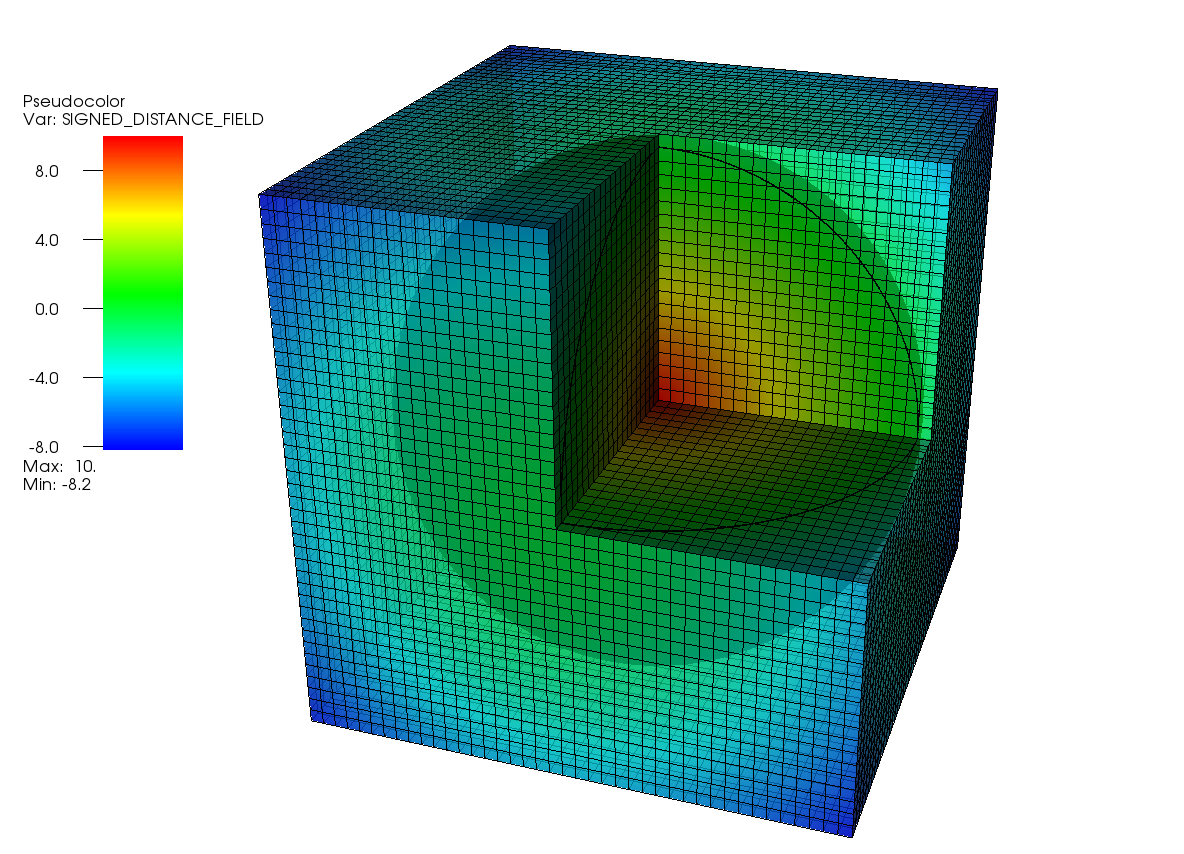
\includegraphics[scale=0.35]{../images/sdf_sphere.png}
  \caption{A visual of a signed distance field with step size 0.5 cm surrounding
    the spherical volume of test case with a radius of 10 cm. Note the reversal
    of the sign convention in comparison to Eq. \ref{eq:sdf}. It is preferable
    to change this when populating the data structure rather than incurring the
    additional computational cost of altering the sign of values for each
    operation at runtime.}
  \end{center}
  \label{fig:sdf_sphere}
\end{figure}

Signed distance values can be retrieved from the structured mesh by determining
which mesh voxel the point lies within. The point's element is accessed by
determining an $<i,j,k>$ index using the point's x, y, and z values divided by
the structured mesh step size. A trilinear interpolation of the mesh element's 8
vertex coordinates and their signed distance values is then used to provide the
signed distance value for the location of interest. As a result, the complexity
of a signed distance value lookup from the signed distance field is
$O(1)$.

As an initial implementation, one signed distance field is generated for each
volume in DAGMC with extents matching the axis-aligned bounding box of the
volume. The signed distance field is represented as a uniform structured mesh
with a signed distance value at each vertex in the mesh as indicated in Fig.
\ref{fig:preconditioner_datastruct}.

\subsection{SDF Population}

Signed distance fields are typically generated using an implicit, analytic
representation, but a suitable data structure for populating the structured mesh
with signed distance values is already in place in the form of DAGMC's bounding
volume hierarchy. It is a more straightforward process to simply use DAGMC's
current closest to location algorithm to generate signed distance values than to
create an implicit surface approximation of the triangle mesh. This method also
maintains a consistency between the intersections found by the ray tracing
kernel and the signed distance field values.

DAGMC's closest to location algorithm returns, among other pieces of
information, the nearest intersection location and the triangle on which this
intersection exists. For each point in the signed distance field mesh, this
algorithm is used to determine the magnitude of the distance value. To
accomplish this, a ray is constructed from query location to the intersection
location. The dot product of this ray vector with the triangle's outward normal
vector is used to determine the sign of the distance value. DAGMC maintains
enough information to consistently orient triangle normals such that they point
outward from the volume they represent. In the rare cases for which the dot
product of these vectors is ambiguous, or zero, DAGMC's point containment
algorithm is used to disambiguate the value's sign.

\section{Utilization Modeling}\label{section:preconditioner_utilization}

In effect, the preconditioner is attempting to check whether or not the particle
will actually cross a surface before explicitly searching for the particle's
intersection with a surface along its current trajectory. If the result of this
preconditioning check is always false and a ray is always fired, then these
checks are only adding to the computational cost of the problem. This will
always occur in volumes filled with void, for example, as particles immediately
travel from one side of a volume to another. As a result, the signed distance field
should be applied selectively depending on each volume's geometric and material
properties for optimal performance and high utilization of the preconditioning
methods.

Ideally, this method will only be applied to volumes in which the data
structure is able to precondition ray fire calls often or with high utilization
of the data structure. The signed distance field is expected to have the biggest
impact in performance when preconditioning next surface intersection queries, as
they are most commonly called in Monte Carlo codes when tracking neutral particles
through the geometry. As such, this type of query is the focus of utilization
measurement for the remainder of this section.

PROVIDE PROOF THAT NEXT SURFACE IS MOST CALLED

\begin{equation}
  U = \frac{ \small \text{Rays Avoided w/ SDF} }{ \small \text{Number of Geometry Queries} } 
   \label{eq:preconditioner_utilization}
%  \caption{Definition of signed distance field utilization as a ray fire preconditioner in DAGMC.}
\end{equation}

As shown in Eq. \ref{eq:preconditioner_utilization}, the utilization, $U$, of
the signed distance field as a ray fire preconditioner can be described as the
number of ray fire calls related to the next surface intersection queries that
are avoided divided by the total number of next surface intersection queries
made by the Monte Carlo code. This value can be quantified using this definition
using debugging tools, such as Valgrind, to determine the number of queries made
in DAGMC and the number of rays fired inside of the subroutine.  It is expected
that in the majority of cases, as the utilization of preconditioning methods
goes up, the performance of the simulation will also improve.



\begin{figure}[ht]
  \centering
  \includesvg{../images/sdf_hydrogen_density_study_util}{\textwidth}
  \caption{Utilization results for a 5 MeV neutron source at the origin of a 10 cm radius
    sphere. Hydrogen density was varied from 0 to 1 $\frac{g}{cm^3}$.}
  \label{fig:sphere_hydrogen_density_study_util}
\end{figure}

To understand this utilization more deeply with respect to material parameters,
the hydrogen density was varied from 0 to 1 $\frac{g}{cm^3}$ in the single-volume
sphere test problem with a 5 MeV neutron point source. For each density, one
simulation was performed without the signed distance field and another with the
signed distance field and preconditioning enabled. Fig.
\ref{fig:sphere_hydrogen_density_study_util} shows the utiilzation results of this study. 

\begin{figure}[ht]
  \centering
  \includesvg{../images/sdf_hydrogen_density_study_perf}{\textwidth}
  \caption{Performance results for a 5 MeV neutron source at the origin of a 10
    cm radius sphere. Hydrogen density was varied from 0.0 to 1.0
    $\frac{g}{cm^3}$. Simulations of 100M histories at each density were
    performed using native MCNP5, DAG-MCNP5 without the signed distance field,
    and DAG-MCNP5 with the signed distance field.}
  \label{fig:sphere_hydrogen_density_study_perf}
\end{figure}

Utilization of the data structure in this study remains high until the hydrogen
density falls to 0.1 $\frac{g}{cm^3}$ at which point a distinct knee appears and
the utilization falls off quickly. Even at the lowest density reached in the
study of 0.01 $\frac{g}{cm^3}$, the utilization of the signed distance field to
avoid ray fire calls is 0.54.


Fig. \ref{fig:sphere_hydrogen_density_study_perf} provides an impression of the
performance of these three implementations converge as the density of the
hydrogen is varied. As the hydrogen density approaches 1.0 $\frac{g}{cm^3}$, a
factor of ~3.5 improvement in runtime is seen in the simulation where the SDF is
applied as a preconditioner. The application of the signed distance field allows
for significantly improved performance until the density drops below 0.1
$\frac{g}{cm^3}$ in agreement with utilization plot. As the material density
decreases, particles quickly leave the geometry after very few collisions. It is
difficult to judge the impact on the performance of this simulation for these
low density values due to the limited size of the geometry and the short lived
histories.  In order to have more control over a simulation's physical
parameters, subsequent experiments were performed using a pseudo Monte Carlo
simulation tool.

\section{Signed Distance Field Utilization Modeling}

In order to characterize utilization of a signed distance field as a
preconditioner for next surface intersection queries in DAGMC, a pseudo Monte
Carlo simulation tool was developed using DAGMC. This tool was used to simulate
different transport scenarios within a spherical geometry using an isotropic
volumetric source and isotropic scattering. Particle histories are terminated
based on a maximum number of collisions or departure from the problem
geometry. Particle distance traveled, $d$, can be represented by either a fixed
distance or by sampling for the standard probability of interaction in a medium
with mean free path, $\lambda$. The tool allows the value of $\lambda$ to be set
directly, enabling a relation between the signed distance field and this value
to be developed with intent for use this relationship as a means for
characterizing appropriate conditions for application of the signed distance
field.

\begin{figure}[!htb]
  \centering
  \includesvg{../images/sdf_fixed_dist_results}{\textwidth}
  \caption{Results of the model for the theoretical utilization limit with the
    results of the simulation for a fixed distance traveled case.}
  \label{fig:sdf_fixed_dist}    
\end{figure}

To begin, simulations were performed for particles with a fixed distance
traveled for varying distances and signed distance field step sizes. Run times
of the simulation are not shown here as the data structure's utilization is the
main focus of this study. The results of the study are shown in
Fig. \ref{fig:sdf_fixed_dist}. As the signed distance field mesh step size
increases, utilization of the data structure decreases due to the increasing
error associated with the interpolation of signed distance values. Additionally,
utilization is expected to decrease with increasing distance traveled. This
decreased utilization is caused by not only the increased distance between the
two particles, but also by the increased probability that both locations will be
closer to surfaces of the sphere and have smaller signed distance values. A
theoretical limit for the utilization is also shown in
Fig. \ref{fig:sdf_fixed_dist}. The development of the analytic form for this
limit will now be discussed.

\begin{figure}[ht]
  \centering
  \includesvg{../images/alpha}{0.3\textwidth}
  \caption{Depiction of model variables.}
  \label{fig:model}
\end{figure}

The utilization of the signed distance field as a preconditioner for ray tracing
operations can be modeled as an evaluation of the combined probability space for
particles with a current position, $\vec{p}$, and a next physics event location,
$\vec{n}$, after traveling a distance, $d$. The fraction of this probability
space in which signed distance values can be used to rule out surface crossings
for next surface intersections is then considered to be the theoretical
utilization of the signed distance field. An initial form for this probability
space can found in Eq. \ref{eq:util_model}.

\begin{equation}
  \label{eq:util_model}
\int_{V_{sphere}}\int_{V_{track}} p_p(r) p_n(d) \, \mathrm{d}V_{sphere}\mathrm{d}V_{track}
\end{equation}

In this model, the starting location of particles, $\vec{p}(r,\phi,\theta)$, is
uniformly distributed, $p_p(r)=1$, throughout a sphere of radius, $R$.  The
location of the next event, $n(d,\alpha,\beta)$, where $d$ is the distance
traveled by the particle, $\alpha$ is the interior angle between the
particle's \textit{position} vector and the particle's sampled direction
vector, and $\beta$ represents an azimuthal angle for directions traveled with
angle of departure, $\alpha$. Fig. \ref{fig:model} depicts these
variables, $r$, $d$, and $\alpha$ more clearly.

The outer integral in Eq. \ref{eq:util_model} represents all possible particle positions within the
geometric sphere and expands to

\begin{equation}
\int_{0}^{R}\int_{0}^{2\pi}\int_{0}^{\pi}\int_{V_{track}} r^2\sin{\phi} \, \mathrm{d}\phi
\mathrm{d}\theta \mathrm{d}r \,  p_n(d) \mathrm{d}V_{track}
\end{equation}

The inner integral over $V_{track}$ then expands to

\begin{equation}
\small \int_{0}^{R}\int_{0}^{2\pi}\int_{0}^{\pi}\int_{0}^{\infty}\int_{0}^{2\pi}\int_{0}^{\pi}
r^2\sin{\phi} \, p_n(d) d^2 \sin{\alpha} \, \mathrm{d}\alpha \mathrm{d}\beta \mathrm{d}d \, \mathrm{d}\phi
\mathrm{d}\theta \mathrm{d}r
\end{equation}

Integration of $\phi$, $\theta$, and $\beta$ can now be performed with
the knowledge that they are symmetric with respect to the problem and
integration of $p_n(d)$ does not rely on them.

\begin{equation}
\small 8\pi^2  \int_{0}^{R}\int_{0}^{\infty}\int_{0}^{\pi} p_n(d) \,
r^2 \, d^2 \sin{\alpha} \, \mathrm{d}\alpha \mathrm{d}d \, \mathrm{d}r
\end{equation}

In order to represent particles traveling a fixed distance, the relationship in Eq. \ref{eq:pn_fixed}
is applied.

\begin{equation}
  \label{eq:pn_fixed}
  p_n(d) = \frac{\delta(d-\lambda)}{d^{2}}
\end{equation}

The evaluation of this integral then gives a representation of all the query
space available to the problem

\begin{equation}
  \label{eq:A_fixed}
\small A = 8\pi^2  \int_{0}^{R}\int_{0}^{\infty}\int_{0}^{\pi} \delta(d-\lambda) \,
r^2 \, \sin{\alpha} \, \mathrm{d}\alpha \mathrm{d}d \, \mathrm{d}r
\end{equation}

and represents all geometric query space, labeled $A$, for a sphere of radius,
$R$ and a fixed distance traveled, $\lambda$.

In order to understand what fraction of this query space is able to be
preconditioned, the condition for avoiding an explicit nearest intersection
search along a particle direction in Eq. \ref{eq:condition} will now be
applied.

\begin{equation}
  SDV(\vec{p}) + SDV(\vec{n}) > |\vec{p}-\vec{n}| + 2\varepsilon(h)
  \label{eq:condition}
\end{equation}
\begin{align*}
 &SDV - \, signed \, distance \, value \, function \\
 &\vec{p} - \, particle's \, current \, position \\
 &\vec{n} - \, particle's \, next \, event \, location \\
 &h - \, mesh \, step \, size \\
 &\varepsilon(h) - \, error \, evaluation \, for \, signed \, distance \, values \\
\end{align*}

This condition establishes that the nearest location to intersection for both
points must be greater than the distance between the two points plus any error
associated with their signed distance values as previously discussed. This
condition is true for some fraction of the next surface queries in a Monte Carlo
simulation, but not all.  This model does not account for error, making it an
idealized model representing the largest utilization possible for any given
pseudo simulation.

\begin{equation}
SDV(\vec{x}) =  R-|\vec{x}|
\end{equation}

Making these substitutions into the inequality gives

\begin{equation}
R-|\vec{p}| + R - |\vec{n}| >   |\vec{p}-\vec{n}|
\end{equation}
The right hand side of this inequality can be described as the distance
traveled, $d$, and the magnitude of $\vec{p}$ can be represented
by the variable $r$.

\begin{equation}
 R-r + R - |n(d,\alpha,\beta)| > d
\end{equation}

Reducing the next event location, $\vec{n}(d,\alpha,\beta)$, into an expression
in terms of $r$, $d$, and $\alpha$ requires further examination of the
problem. Because the coordinates of $n$ depend on the current particle position,
the magnitude of $n$ with respect to the geometry origin must be obtained to get
a correct form for the signed distance value. Again, Fig. \ref{fig:model} depicts the
value of $n$ graphically for reference. The magnitude of n can then be described
using the law of cosines as

\begin{equation}
|n(d,\alpha,\beta)| = \sqrt{r^2 + d^2 - 2rd \cos{\pi-\alpha}}
\end{equation}
inserting this into the inequality gives

\begin{equation}
R-r + R - \sqrt{r^2 + d^2 + 2rd \cos{\alpha}} > d
\end{equation}

The inequality has now been reduced to the three variables seen in
Eq. \ref{eq:A_fixed}:$r$, $d$, and $\alpha$. This inequality can be applied to
construct limits of integration representing boundaries of space in which the
SDF can be utilized. By rearranging the inequality, a limit on the angle of
departure, $\alpha$, from the particle's position can be derived.

\begin{equation}
\alpha_{min} > \arccos\Bigg ( \frac{(2R-r-d)^2-d^2-r^2}{2 d r} \Bigg )
\end{equation}

\begin{figure*}[ht]
  \centering
  \includesvg{../images/model_cases_fixed_distance}{\textwidth}
  \caption{Depiction of modeling cases. Left: an example of a track for which
    $d < R - r$. Middle: an example of a track for which $R-r < d < R$ and can be
    preconditioned.  Right: an example of a track for which $R-r < d < R$ and
    cannot be preconditioned.}
  \label{fig:modeling_cases}
\end{figure*}

This condition on alpha can be interpreted as a minimum interior angle that the
particle's trajectory must take relative to the particle's position vector,
$\vec{p}$, for a distance traveled, $d$, for a ray fire to be avoided and the
preconditioner to be utilized. The examination of this condition as a function
of the distance traveled for various values of $r$ results in some conclusions
about how signed distance values are being utilized.

\begin{figure}
\centering
\includesvg{../images/alpha_r}{\textwidth}
\caption{Plot of minimum angle of departure restriction for particles with
various radial positions, $r$, in a sphere with R = 100 cm and varying distances traveled.}
\end{figure}

The inequality is undefined until the distance reaches a value $d = R- r$. This
is because the angular limit only needs to be applied to areas of the query
space in which the distance traveled is large enough to violate the above
condition as depicted in Fig. \ref{fig:modeling_cases}. A violation of this
limit may only occur when a particle travels far enough to reach the geometric
sphere boundary along the current position vector as if it were moving directly
toward the boundary of the sphere. An additional interesting feature of this
plot is the convergence of all the curves on $\pi$ as $d$ approaches $R$. The
convergence on $\pi$ indicates that as the distance traveled approaches $R$ the
only direction that the particle can move is back toward the origin along the
position vector. It also defines a maximum distance a particle can travel in the
sphere and still be preconditioned using signed distance values. Intuitively
this makes sense as the maximum chord length of a sphere is $2R$, and once a
particle travels a distance $R$ the sum of the signed distance values can then
be no larger than $R$ and the condition for utilization in Eq. \ref{eq:condition} is
violated. Hence all curves go to zero at $\lambda = 100 cm$ in
Fig. \ref{fig:sdf_fixed_dist}.

In order to account for the fact that the form of $\alpha_{min}$ is undefined
until $d = R-r$, a Heaviside function is applied before applying it as a limit
on the particle's angle of departure from the position vector. Similarly,
because the $\alpha_{min}$ condition is undefined after $d=R$ a Heaviside
function is used to limit the condition to $\pi$ for any distances traveled
larger than $R$.

\begin{equation}
  \small
  \begin{split}
  \alpha_{min} =& (H(d-(R-r))-H(d-R)) \arccos\Bigg ( \frac{(2R-r-d)^2-d^2-r^2}{2 d r} \Bigg ) \\
  &+ \pi \, H(d-R)
  \end{split}
\end{equation}


By inserting this condition as a lower limit of the $d\alpha$ integration,
Eq. \ref{eq:subs_a_cond} will give all utilized space, $US$, in the query space
of the simulation.

\begin{equation}
\small US = 8\pi^2  \int_{0}^{R}\int_{0}^{\infty}\int_{\boldsymbol{\alpha_{min}}}^{\pi} \delta(d-\lambda) \,
r^2 \, d^2 \sin{\alpha} \, \mathrm{d}\alpha \mathrm{d}d \, \mathrm{d}r
\label{eq:subs_a_cond}
\end{equation}

Evaluating this integral and dividing by all query space gives the
following form for the theoretical limit of signed distance field utilization as a
preconditioner for ray firing

\begin{equation}
U_{theoretical} = \frac{US}{A} =  \frac{(1-H(\lambda-R))(2R-\lambda)(R-\lambda)}{2R^2}
\end{equation}

It can be seen in Fig. \ref{fig:sdf_fixed_dist} that this utilization limit
works well as an upper limit for the simulation results using various signed
distance field mesh resolutions. As the step size of the mesh approaches zero,
so does the evaluation of the error, resulting in the same utilization curve
with varying distance traveled, $\lambda$, as in the analytic form developed
here. Future work will include the comparison of this utilization limit to other
single-volume geometries using dimensionless parameters to determine if the
model above can be used to predict signed distance field utilization in other
geometries as well.

%% After the agreement of the simulation results and analytic model for signed
%% distance field utilization for the fixed distance traveled case, the simulation
%% was used to produce a similar set of results in which the distance is
%% sampled based on the standard probability for distance to interaction in a
%% medium with a cross section, $\Sigma$, or mean free path $\lambda
%% =1/\Sigma$. This results in the probability distribution function shown in
%% Eq. \ref{eq:pn_sampled} for the particle distance traveled in this scenario.

%% \begin{equation}
%%   \label{eq:pn_sampled}
%% p_n(d) \propto \frac{e^{-\Sigma d}}{d^{2}} = \frac{e^{-\frac{d}{\lambda}}}{d^{2}}
%% \end{equation}

%% \begin{figure}[ht]
%% \centering
%% \includesvg{../images/sdf_sampled_dist_results}{0.5\textwidth}
%% \caption{Results of the model for the theoretical utilization limit with the
%% results of the simulation for a sampled distance traveled case.}
%% \label{fig:sdf_sampled_dist}
%% \end{figure}

%% %has to be in this section for latex reasons. grumble grumble...
%% \begin{table*}[!h]
%%   \centering
%%   \begin{tabular}{lcccc}
%%           \multicolumn{5}{l}{\textbf{\textit{Source Location:}} <0,0,-1>} \\
%%           \textbf{Implementation} & \textbf{ctme (min)} & \textbf{wall time
%%             (min)} & \textbf{time ratio} & \textbf{precond. utilization}\\
%%           \hline
%%           MCNP6 & 0.17 & 0.14 & 1 & N/A \\
%%           DAG-MCNP6 & 1841.33 & 1841.33 & ~11,000 & N/A \\
%%           DAG-MCNP6 w/ SDF & 0.48 & 0.46 & 2.82 & 0.94\\
%%           \multicolumn{5}{l}{} \\
%%           \multicolumn{5}{l}{\textbf{\textit{Source Location:}} <0,0,10>} \\
%%           \textbf{Implementation} & \textbf{ctme (min)} & \textbf{wall time
%%             (min)} & \textbf{time ratio} & \textbf{precond. utilization}\\
%%           \hline
%%           MCNP6 & 0.18 & 0.18 & 1 & N/A \\
%%           DAG-MCNP6 & 11.12 & 11.16 & 62 & N/A \\
%%           DAG-MCNP6 w/ SDF & 0.50 & 0.52 & 2.89 & 0.96 \\
          
%%   \end{tabular}
%%   \caption{Performance results for an MCNP6 test case involving electron
%%     transport of a 1 keV-100 keV photon source incident on an Fe/W target. 5,000
%%     histories were run in this test problem.}
%%   \label{tab:inp066_results}
%% \end{table*}

%% Following the same process as in the fixed distance case by plugging Eq. \ref{eq:pn_sampled} into
%% Eq. \ref{eq:subs_a_cond}, the utilization form for the sampled distance case is
%% shown in Eq. \ref{eq:sampled_limit}.

%% \begin{equation}
%%   \label{eq:sampled_limit}
%%   U_{theoretical} = \frac{US}{A} = \frac{ \frac{1}{2} \lambda(R - 2 \lambda) e^{\frac{-R}{\lambda}} + \lambda^2 - \frac{3}{2} R \lambda + R^2 }{R^2}
%% \end{equation}

%% The results of this set of simulations can be seen in
%% Fig. \ref{fig:sdf_sampled_dist}. In this scenario, it is not expected that the
%% utilization will approach zero when $\lambda = 100\, cm$, as the actual distance
%% sampled may be considerably less than the provided mean free path for the
%% simulation. Overall utilization values in this scenario for $\lambda$ from 0 to
%% 100 cm remain higher than the corresponding fixed distance simulation cases as
%% is expected in a sampled distance case. Utilization values remain high for
%% relatively large increases in mesh step size, $h$. This is important to
%% application of the data structure given concerns regarding its potentially high
%% memory footprint for large volumes. For example if the utilization of the signed
%% distance field drops $~20\%$ when going from a step size of 1 cm to 6.21 cm, but
%% the memory footprint of the data structure will have decreased by a factor of
%% $6.21^3$ or $239.5$ as well. The optimization of the mesh step size with respect
%% to its effect on utilization will also need to be included in future models of
%% the utilization.

The fixed distance traveled scenario provides a nice baseline for agreement
between the computational results and the model, but a more realistic scenario
is required before attempting to apply the model as a predicitive utility for
application of the SDF in true Monte Carlo codes. The most useful alteration of
the current simulation scenario is to move from a fixed distance distance to a
sampled distance based on the standard probability for distance to interaction
in a medium given a cross section, $\Sigma$.

$$ p = e^{-\Sigma d} = e^{-\frac{d}{\lambda}} $$

where in this case now $\lambda$ represents the mean free path of the particle in the medium

In simulation, distances are now sampled as

$$ d = -\lambda ln(p) $$

where p is randomly sampled with a uniform distribution between 0 and 1

Inserting this definition for the particle distance into the integrals above
gives

$$ \frac{dp}{dd} = -\frac{p}{\lambda} $$
$$ d = 0 \rightarrow p = 1 $$
$$ d = D \rightarrow p = 0 $$

$$ \int_{0}^{R}\int_{0}^{2\pi}\int_{0}^{\pi}\int_{1}^{0}\int_{0}^{2\pi}\int_{0}^{\pi}
-r^2\sin{\phi} \, \lambda p ln(p)^2 \sin{\alpha} \, \mathrm{d}\alpha \mathrm{d}\beta \mathrm{d}p \, \mathrm{d}\phi
\mathrm{d}\theta \mathrm{d}r $$

This integral can then be evaluated to give the entirety of the geometry space
for the problem

\begin{center}
All Query Space = $\frac{4}{3} \lambda \pi^2 R^3$
\end{center}

To find the portion of utilized space for a given $R$ and $\lambda$ one can
apply the same methods from the fixed distance case, for each particle position
within the sphere there will still be two scenarios - one in which the distance
traveled exceeds $R-d$ and another in which it is less than $R-d$. The difference
now is d has become a distrubution rather than a constanct value, so as the
distance traveled changes the queries will fall into either category for a
single particle position.

Another way of viewing of viewing this condition in the case of a varying
distance is to define these same categories based on the distance traveled. Now
rather than defining how the angular condition is applied based on position, the
angular condition will be applied based on the distance the particle travels.

$$ d < R-r : \alpha_{min} = 0 $$
$$ d > R-r : \alpha_{min} = \arccos\Bigg ( \frac{(2R-r-d)^2-d^2-r^2}{2 d r} \Bigg
) $$

It is interesting to examine plots of the angular limit with varying distance as
seen in Fig. \label{fig:alpha_min}

\begin{figure}[ht] \label{fig:alpha_min}

\centering
\includesvg{alpha_r}{1\textwidth}
\caption{Plot of mininum angle of departure restriction for particles with
various radial positions and varying distances traveled.}
\end{figure}

The entry point of each curve in the plot represents the minimum distance
necessary to enter the $d > R-r$ region and begins to apply an agular
restriction. Note that each of these approach a mininmum angle of $\pi$ as the
distance traveled approaches $R$ (100cm). This represents a particle traveling
back towrd the origin along the sphere's larges chord with length $2R$ and,
again,the maximum distance a particle can travel before the SDF can no longer be
utilized.

Now that the distance traveled is being used to construct these two regions in
the model, this integral must be separated into two pieces, one with limits of $0$
to $R-r$ and another with limits $R-r$ to $R$. Based on the distance sampling
distribution, these values become

$$ d_{min} = R-r \rightarrow p_{max} = e^{(-\frac{(R-r)}{\lambda})} $$
$$ d_{max} = R   \rightarrow p_{min} = e^{(-\frac{R}{\lambda})} $$

and our integral becomes

$$ \int_{0}^{R}\int_{0}^{2\pi}\int_{0}^{\pi}\int_{1}^{p_{max}}\int_{0}^{2\pi}\int_{0}^{\pi}
-r^2sin(\phi) \, \lambda p ln(p)^2 sin(\alpha) \, \mathrm{d}\alpha \mathrm{d}\beta \mathrm{d}p \, \mathrm{d}\phi
\mathrm{d}\theta \mathrm{d}r + $$
$$ \int_{0}^{R}\int_{0}^{2\pi}\int_{0}^{\pi}\int_{p_{max}}^{p_{min}}\int_{0}^{2\pi}\int_{alpha_{min}}^{\pi}
-r^2\sin{\phi} \, \lambda p ln(p)^2 \sin{\alpha} \, \mathrm{d}\alpha \mathrm{d}\beta \mathrm{d}p \, \mathrm{d}\phi
\mathrm{d}\theta \mathrm{d}r $$

The evaluation of this integral divided by the full geometry query space for the
distance sampling scenario after the $c=\frac{R}{\lambda}$ replacement is

$$U(c) = \frac{1}{4}\frac{(4 c^2-6) c^2e^{-2c} - (c^3-c^2-\frac{3}{2}
c+3)4ce^{-2c}+(-2 c^3+2c^2+9c-6) e^{-2c}+4c^2-9 c+6}{c^2}$$

\begin{figure}[ht] \label{fig:sdf_sampled_dist}
\centering
\includesvg{../images/sdf_sampled_dist_results}{\textwidth}
\caption{Results of the model for the theoretical utilization limit with the
results of the simulation for a fixed distance traveled case.}
\end{figure}

Unfortunately the predictive model for the sampled distance scenario is not
consistent with the simulation results, and under predicts the utilization of
the SDF significantly. It is quite possible that utilization in either th interior or exterior
resion of the sphere is being under represented. Regardless of the cause, examining the contribution to
utilization from each of these regions (shown in
Fig. \label{fig:util_region_contributions}) is an interesting endeavor.


\begin{figure}[ht] \label{fig:util_region_contributions}
\centering
\includesvg{../images/util_contributions}{\textwidth}
\caption{A plot of the total predicted utilization along with the contriubtions
from the inner region ($d < R-r$) and outer region ($d > R-r$).}
\end{figure}

Figure \ref{fig:util_region_contributions} depicts the utilization of the SDF
data structure for various values of the mean free path, $\lambda$.
When $\lambda$ is very small, particles' next event locations
rarely reach the outer region condition of $ d > R - r $. As $\lambda$ increases, particles are
more likely to enter that region and its contribution increases greatly. Then
as particles begin to travel distances on the order of the sphere radius the
utilization decreases. The interior region utilization acts as one would
expect. When particles travel small distances with respect to the sphere radius,
there is high utilization, but as the particles begin to travel further its
utilization rapidly decreases. The contribution from the outer region defines the
significance of using both the current position signed distance value as well as the
next event location's signed distance value to precondition ray fire calls in DAGMC.

\subsubsection{Modeling with Error Evaluation}

Thus far, the error associated with the tri-linear interpolation used to recover
signed distance values from the signed distance field has been ignored. In
order to optimize step size of the uniform mesh making up the signed distance
field, it is important to take this error into account when predicting the
utilization of the data structure.

As seen in Figure \ref{fig:sdf_sampled_dist}, the step size of the mesh can
significantly impact the utilization of the data structure and in turn the
overall performance of the simulation. It is important to use a step size which
will not artificially limit the effect of the data structure, but the signed
distance field is a dense data structure and uses a considerable amount of
memory. The memory usage of the signed distance field is inversely proportional
to the cube of the mesh step size ($\alpha \frac{1}{h^{3}}$). Therefore it is
important to consider the impact that this error will have on the utilization
of the data structure.

The expansion of Eq. \ref{eq:condition} with the error term maintained results in
a new condition for the minimum angle of departure ($\alpha_{min}$) shown in
Eq. \ref{eq:min_alpha_w_error}

\begin{equation}
\small
\begin{split}
\alpha_{min} =& (H(d-(R-r-\epsilon))-H(d-(R-\epsilon))) \arccos\Bigg ( \frac{(2R-r-d-2\epsilon)^2-d^2-r^2}{2 d r} \Bigg ) \\
&+ \pi \, H(d-(R-\epsilon))
\end{split}
\label{eq:min_alpha_w_error}
\end{equation}

This formulation of $\alpha_{min}$ can be used directly in the integration described
in Eq. \ref{eq:subs_a_cond}. The final form of the model after the integration being:

$$ US_{sampled} = \frac{(R-\epsilon) (\frac{1}{2} \lambda ( R - 2\lambda - \epsilon ) e^{\frac{-R + \epsilon}{\lambda}} +
\lambda^{2} - \frac{3}{2}\lambda(R - \epsilon) + (R-\epsilon)^{2})}{R^3}$$


%% For a direct evaluation of the utilization based on
%% the mesh step size, $h$, the formula for the error can be substituted for
%% $\epsilon$ to give

%% \begin{equation}
%% \small
%% \begin{split}
%% \alpha_{min} =& (H(d-(R-r-\sqrt{3}h))-H(d-(R-\sqrt{3}h))) \arccos\Bigg ( \frac{(2R-r-d-2\sqrt{3}h)^2-d^2-r^2}{2 d r} \Bigg ) \\
%% &+ \pi \, H(d-(R-\sqrt{3}h))
%% \end{split}
%% \end{equation}

This updated model was then compared to pseudo-simulations using sampled
distances for the next physics event location. The result of this can be seen in
Figure \ref{fig:sdf_util_sampled_distance_w_error}.

\begin{figure}[ht]
  \centering
  \includesvg{../images/sdf_util_sampled_distance_w_error}{\textwidth}
  \caption{Theoretical limits for SDF utilization accounting for error
    evaluation plotted with simulation results for varying mesh step sizes.}
  \label{fig:sdf_util_sampled_distance_w_error}
\end{figure}

\subsubsection{Extension to other geometries}

To apply this model to other geometries, the mean free path and mesh step size
were normalized using a measure of the free space in a volume compared to its
surface area, the average chord length ($R_av$) \cite{Wigner_1981}.  This value
can be defined as seen in Eq. \ref{eq:average_chord_length}.

\begin{equation}
\centering
 R_{av} = \frac{4V}{S}
 \label{eq:average_chord_length}
\end{equation}
\begin{align*}
 &V \, - \, Volume \\
 &S \, - \, Surface \, Area
\end{align*}

The mean free path and mesh step size can be normalized by this value to
represent values relative to the geometry. Normalizing the mean free path to the
average chord length is a way of describing the probability that a particle will
reach the surface of the volume in a way that is independent of the distance
traveled by the particles and the explicit geometry \cite{Mazzolo_2014}. Normalizing the mesh step
size using the average chord length is a description of how much of the particle
track the error will occupy. This allows us to now describe the space in a
[n=(0,1),c=(0,1)] domain for an arbitrary geometry, particle distance traveled,
and mesh step size.

This normalization allows a way to compare the model developed above to compare
utilization results for other geometries, which will be important in assessing
the utilization of the SDF in more geometrically complex volumes. In order to
test the extension of this analytic model to other geometries, the pseudo
simulation for various path lengths was repeated for cylinder and cone
geometries. The results of the utilization model and simulation results can be
found in Figures INSERT REFERENCE TO FIGURES HERE. The results of these tests
indicate that the utilization model can be used to predict the data structure's
utilization for other geometries as well, though with some limitations.

For small values of $n$, the utilization model is much closer to the simulated
result. As the value of $n$ increases, however, the model no longer agrees well
with the simulated results. The reason for this is that the analytic model
breaks down for values of $n$ which are outside of the limits set by the
$\alpha_{min}$ condition . In the spherical case this occurs when the error
evaluation exceeds $R$, meaning that zero utilization of the data structure is
expected. 

$$ \epsilon(h) > R $$
$$  \sqrt{3}h = R $$

\begin{equation}
 h = \frac{R}{\sqrt{3}}
\label{eq:error_condition_sphere}
\end{equation}

For this condition, any evaluation of the error will exceed the maximum distance a
particle can travel and still be utilized, as described previously in this
chapter. To extend this limitation to other geometries, the average chord length
will again be used as a surrogate for the sphere radius in representing the upper
limit of utilization for an arbitrary geometry. For the spherical case, the
average chord length is 

$$R_{av} = \frac{4}{3}R $$

$$ R = \frac{3}{4} R_{av} $$

This can then be substituted into Eq. \ref{eq:error_condition_sphere}
to obtain relationship of the mesh step size to the geometry for an upper limit
of $h$ when applying this model.

\begin{equation}
 h < h_{max} =  \frac{3}{4\sqrt{3}} R_{av} 
\label{eq:sdf_max_h}
\end{equation}

Eq. \ref{eq:sdf_max_h} provides a value for the maximum allowed step size for
which the utilization model in an arbitrary geometry. While unlikely that a step
size this large would be applied in practice, it is important to understand the
limitations of this model if it is to be used in an automated process for
application of the data structure either on-the-fly or as a preprocessing step
before running particle histories.

\subsubsection{Application in Simulation}

The geometry-agnostic version of the utilization model was used to create a
\textit{de facto} analysis script for predicting the SDF's utilization in
production DAG-MCNP models. This analysis uses information about the average
particle track length for each volume as the input mean free path for the
utilization model. This information is gathered from Table 126 provided in MCNP
output files from previous DAGMC simulations of the geometry. The input for the
average chord length of each cell was calculated using DAGMC methods
\textit{measure\_volume} and \textit{measure\_area} for each cell in
question. The mesh step size was treated as a variable used to optimize either
the memory usage of the data structure or the utilization of the data structure
depending on options passed into the script. The output of the script then
describes inputs to the utilization model, the predicted utilization of the data
structure, and an estimate of data structure's memory usage.

This analysis script was used to examine several models to search for volumes
with a significant impact on the simulation, but the addition of the data
structure had only small effects on the performance of the simulation. One
additional factor that the script takes into account is the number of collisions
in the volumes it is examining. Despite the fact that the collision density of
the transport in a given volume may be high relative to its average chord
length, if a small percentage of the transport occurs in that volume, then the
benefits of applying the SDF are diminished. As an estimate of this, the ratio
of collisions a given volume to the total number of collisions in the sumulation
was used as an estimate for the proportion of geometric queries occuring in the
volume.  Additionally, it has been found through profiling of various models
that as the collision density increases, the proportion of the runtime spent
querying the geometry is small relative to the time spent calling physics
subroutines.

\sdfModel{ITER}{
  The International Thermonuclear Experimental Reactor (ITER) is a demonstration
  nuclear fusion device currently under construction in southern France. An
  analysis of DAGMC was performed at the University of Wisconsin - Madison to
  determine the dose rate to maintenance workers after shutdown of the
  facility.
}

%% \sdfModel{FNG} {
%%   The Frascati Neutron Generator (FNG) is a neutrom source device which uses a
%%   tritium gas target to generate 2.5-MeV neutrons at a fluence of 1E11 n/s.
%% }

\sdfModel{nTOF}{
  The neutron Time Of Flight (nTOF) model is a project underway at the Institute
  for Science and International Security (ISIS) in the United Kingdom. The aim
  of this project is to determine neutron energies by measuring the time it
  takes neutrons to travel from one detector to another.
}

\sdfModel{SHINE}{
  The SHINE facility is a device which uses a beam fusion device to produce
  14.1-MeV neutrons and irradiate an aqueous uranium solution to produce
  molybdenum 99 for use in medical imaging.
}

\sdfModel{Spallation Neutron Source}{
  The Spallation Neutron Source (SNS), located at Oak Ridge National Laboratory,
  in which protons are accelerated to high energies (~1 GeV) and directed into a
  mercury target to produce thermal neutrons for various research applications.
  }

\begin{table}[H]
  \small
  \makebox[\textwidth][c]{
    \begin{tabular}{l c c c c}
      \toprule
      \textbf{DAGMC Model} & \textbf{Histories Simulated} & \textbf{Predicted Utilization (\%)} & \textbf{Actual Utilization (\%)} & \textbf{Timing Ratio} \\
      \hline
      ITER                 & 1M                           & 37.1                                & 40.1                             & 0.86                  \\
      nTOF                 & 10k                          & 62.9                                & 66.2                             & 0.71                  \\
      SHINE                & 500k                         & 60.1                                & 48.2                             & 0.64                  \\
      SHINE$^{*}$          & 500k                         & 60.1                                & 56.5                             & 0.74                  \\
      SNS                  & 10k                          & 31.0                                & 2.1                              & 1.00                  \\
      \bottomrule
    \end{tabular}
    }
    \caption{A summary of SDF application to several production DAGMC models.}
    \label{tab:sdf_prod_summary}
\end{table}


\begin{table}[H]
  \small
  \makebox[\textwidth][c]{
    \begin{tabular}{l c c c c}
      \toprule
      \textbf{Model} & \textbf{Particle Types}                  \textbf{Next Surface} & \textbf{Closest Surface} & \textbf{Point in Volume} \\
      \hline
      SNS            & $\alpha$,p,$\gamma$,$\beta$,$^{3}H$,n... & 99.1\%                & < 0.1\%                  & 0.8\%                    \\
      nTOF           & p,$\gamma$,n                             & 99.4\%                & 0.5\%                    & 0.1\%                    \\
      ITER           & n                                        & < 0.1\%               & 0 \%                     & 99.99\%                  \\      
      SHINE          & n                                        & 99.9\%                & 0\%                      & < 0.1\%                  \\
      \bottomrule
    \end{tabular}
  }
  \caption{An examination of relative number of calls to the various Monte Carlo
    geometric queries for several DAGMC production models.}
  \label{tab:geom_query_ratios}
\end{table}  


Despite these various factors diminishing the effects of the data structure, a
volume in the medical isotope production model from SHINE (shown in Figure
\ref{fig:shine_sdf}) was determined to be a suitable candidate for SDF
application.

\begin{figure}
\centering
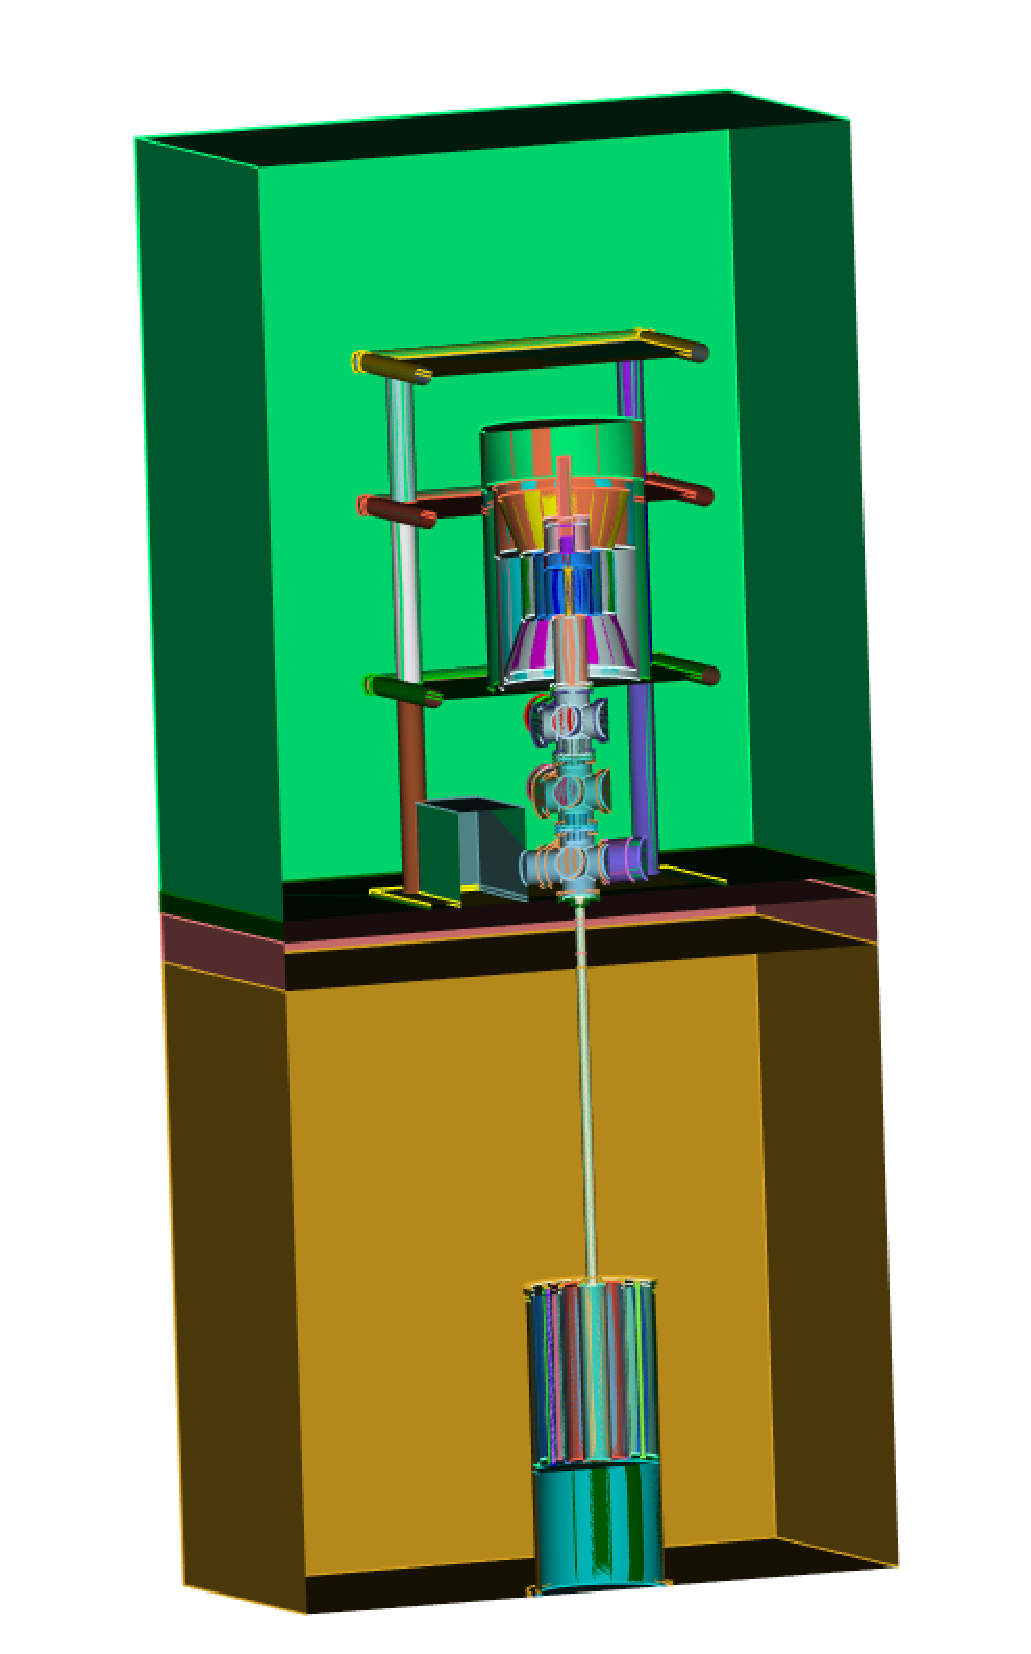
\includegraphics[width=0.4\textwidth]{SHINE.eps}
\caption{A cutaway view of the SHINE model used for demonstration of the SDF
  data structure.}
\label{fig:shine_sdf}
\end{figure}

A signed distance field with a 0.1 cm step size was applied to volumes near the
bottom of the model which contain both an aqueous solution of uraniaum sulfate
and a surounding light water moderator. As outlined in Table
\ref{tab:shine_sdf_result}, the resulting improvement in performance for a
simulation of 500,000 particles was approximately 35\% of the total runtime.

\begin{table}[H]
\centering
\begin{tabular}{c c c}
  \toprule
  \textbf{Implementation} & \textbf{Runtime (min)} & \textbf{Timing Ratio} \\
  \hline
  DAG-MCNP                & 76.14                  & 1.00                  \\
  DAG-MCNP w/ SDF         & 49.28                  & 0.65                  \\
  \bottomrule
\end{tabular}
\caption{Timing results for 500k particle histories of the SDF demonstration on
  the SHINE medical isotope production model.}
\label{tab:shine_sdf_result}
\end{table}

\section{Performance Mitigating Factors}\label{sec:sdf_limitations}

In the majority of the production models to which SDF geometry query
preconditioning was applied, the effect on the overall performance of the
simulation is much smaller than what was seen in the simple test cases. This is
due to a variety of factors, each of which is demonstrated by one of the models
in that table.

\subsection{Physics Dominant Simulations}\label{subsec:sdf_phys_dominant}

The nTOF model was selected as a charged particle transport demonstration. The
SDF was expected to be extremely beneficial in this scenario due to the high
collision density of charged particle transport relative to the size of certain
volumes in the problem. The computational time spent on the detailed of these
charged particles physics tends to dominate the runtime of the simulation,
leaving little room for improvement in the overall simulation runtime by
reducing geometric query costs.

As a neutral particle example of this occurs in SHINE as well. In order to
reduce the amount of time spend in the MCNP kernel for this calculation,
group-wise cross-sections were specified for all materials in the problem. This
allowed the SDF to have a more significant impact on the simulation runtime, but
may not be desirable if continuous energy cross sections are necessary for a
higher fidelity result.

\subsection{Utilization Model Assumptions}\label{subsec:sdf_util_model_limits}

There are some cases in which the SDF utilization model is inaccurate. The
calculation of the average chord length and average track length are assumed to
be true over the entirety of the volume in question. In reality, these values
will vary throughout the volume's domain. In cases where the local value of the
average chord length is smaller than predicted, the utilization model will overestimate
the SDF utilization. An example of this was found in the SNS test model.

A volume representing the mercury manifold in the SNS model was identified as a
good candidate for SDF application. The SDF analysis model estimates the
utilization of the SDF data structure under the assumption that the distribution
of particle interactions in the volume is uniform. In this case, particle
interactions occur mostly in regions of the volume where the local average chord
length is smaller than the average chord length of the entire volume. This
reduces the effectiveness of the SDF for the step size suggested by the input
script. Additionally, an SDF which would provide better utilization would
require a prohibitively small mesh step size in terms of the memory usage of the
data structure. These factors mean that this volume and in turn the SNS
simulation itself doesn't make it a candidate for application of the SDF as a
geometry query preconditioner.

\begin{sidewaysfigure}[h]
  \centering
  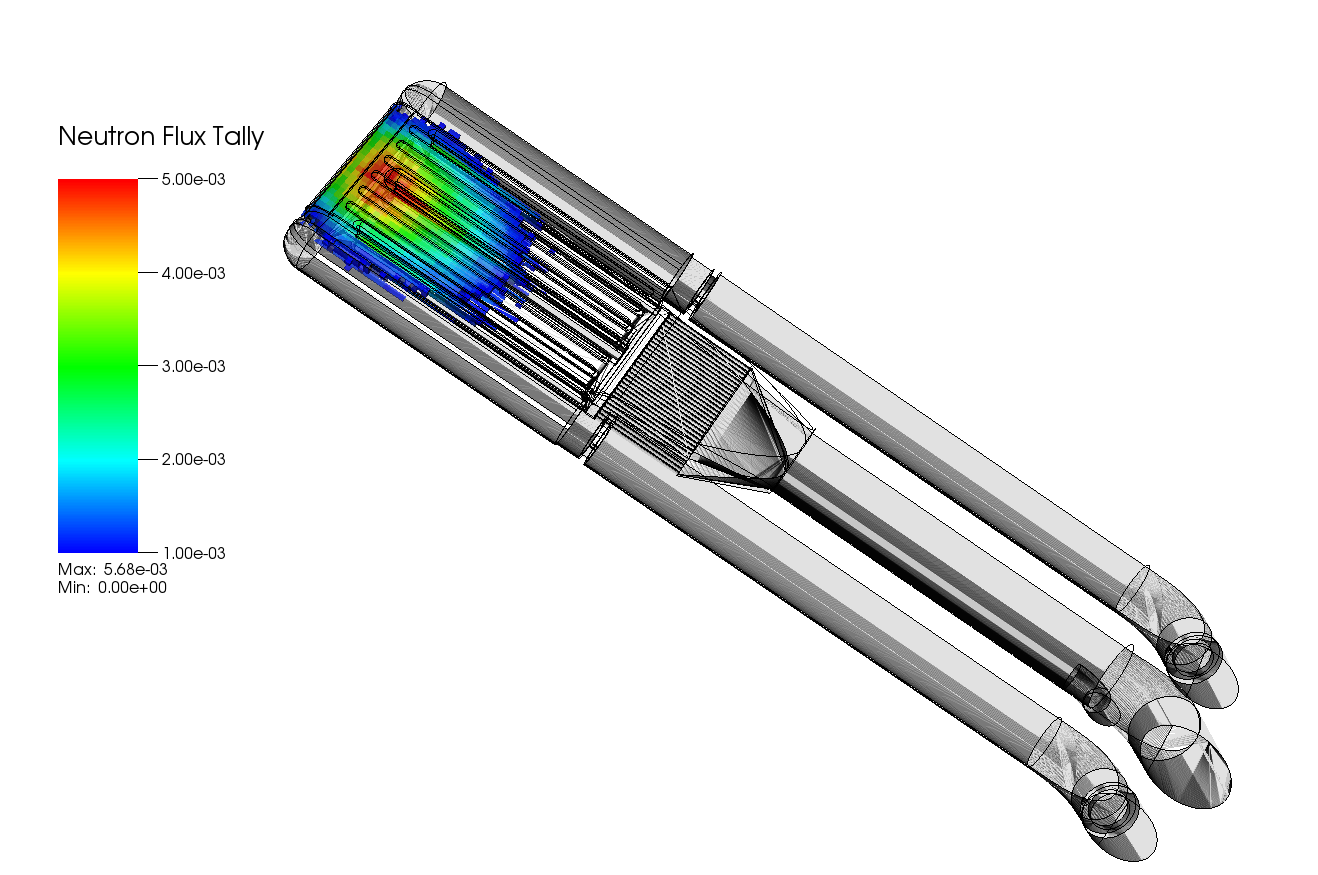
\includegraphics[width=\textwidth]{sns_vol16_flux.png}
  \caption{Example of utilization model limitation due to a small local average chord length
    in the region of high collition density.}
  \label{fig:sns_low_util}
\end{sidewaysfigure}

\subsection{Surface Mesh Complexity}\label{subsec:sdf_tree_depth}

In Section \ref{subsec:sdf_phys_dominant} limitations of the SDF impact on the
nTOF simulations were cited as related to the time spent in physics subroutines,
but the faceting of the particular volume which the SDF was applied to may play
a role as well. The volume's faceting contained a relatively small number of
triangles. This in turn means that the generated BVH for this volume was
relatively shallow. The relative improvement in performance when avoiding a ray
traversal is directly related to this tree depth. While the complexity of a BVH
search is $O(log\, N_{tri})$, the cost relative to the $O(1)$ look-up of a signed
distance value in the SDF becomes small as N becomes small, limiting the
effectiveness of the SDF regardless of the utilization.



\chapter{SIMD MOAB Bounding Volume Hierarchy}\label{ch:simd_bvh}


\section{Introduction}

As established in Section \ref{sec:problem-statement}, the dominant source of
additional runtime in DAGMC is spent in the ray tracing process used to satisfy
the Monte Carlo geometry queries outlined in Section \ref{sec:mc-geom-queries}.
The focus of the work in this chapter is improvements on the performance of the
ray tracing process through the application of SIMD-oriented programming in the
bounding volume hierarchies used in DAGMC. Some preliminary work was performed
in this area by replacing the ray tracing kernel used in DAGMC (MOAB's oriented
bounding box tree) with a kernel produced by Intel, called Embree.

\section{Linking DAGMC with Intel's Embree}\label{sec:embree}

Embree is the result of a an effort to produce a performant CPU-based raytracer
as a demonstration of the expanding capabilities of modern CPU architectures
\cite{Wald_2014}. In both construction and traversal of BVHs, Embree takes
advantage of many of the latest developments in BVH research by using modern
chipset architecture capabilities via vectorization at an implementation level
as described in Section \ref{subsec:arch} of this work. The combination of these
effects leads to a very powerful raytracing tool in terms of performance, as
demonstrated by the many projects which have incorporated Embree as their
production ray tracing kernel such as Corona, Autodesk, FluidRay, and
Brighter3D.As a result of its success in other areas, Embree was selected to be
applied in DAGMC to satisfy geometric queries for MCNP. The resulting
combination of these tools will be reffered to as EmDAG.

\subsection{Transferring DAGMC Model's to Embree Scenes}%%Status:Done%%

The process of employing Embree as DAGMC's ray tracer begins by establishing an
equivalent representation of the MOAB mesh in Embree. In comparison to MOAB,
Embree is limited in its ability to represent the underlying topological
structure of a model. This topology is necessary and used advantageously during
particle tracking in DAGMC by reducing the set of triangles queried to those of
the particle's current volume and thus reducing the number of point containment
queries. However, a method was discovered to represent enough of the topology to
meet the requirements of DAGMC transport. The highest level representation in
Embree is referred to as a scene. Each scene may contain one or more geometries
or triangle surface meshes. Fortunately, this system is enough to create a
workable representation of DAGMC meshes in which MOAB volumes are the equivalent
of Embree scenes and MOAB surfaces are represented in their respective scenes as
surfaces. This method provides a one-to-one mapping of MOAB volumes and surfaces
to their corresponding entities in Embree and allows all topology-based
operations to proceed inside of DAGMC in their usual manner. In this way, the
requirement for topological information in DAGMC at the surface and volume level
is met. Next, transfer of the primitive mesh data is considered.

Scenes do not share mesh data as volumes are able to do in MOAB, so the triangle
connectivity of each surface is reproduced in each scene they belong
to. Fortunately, Embree does allow the sharing of vertices between scenes. In
order to take advantage of this feature, all of the vertices in the MOAB mesh
are provided in the Embree instance as a global vertex buffer. Surfaces from all
scenes can then be defined by a connectivity of vertices from this global pool
of points. This method guarantees that the each surface can be represented by
the same set of stored vertices in each scene it belongs to giving the exact
same representation in each scene. It greatly simplifies particle tracking by
guaranteeing that the same surfaces will not overlap each other in the different
scenes they are a part of by doing the conversion of points from the MOAB
database to Embree only once. Additionally, this method will maintain
watertightnes at the boundaries between surfaces ensuring the same model
fidelity as the representation in MOAB.

\begin{figure}
  \centering
  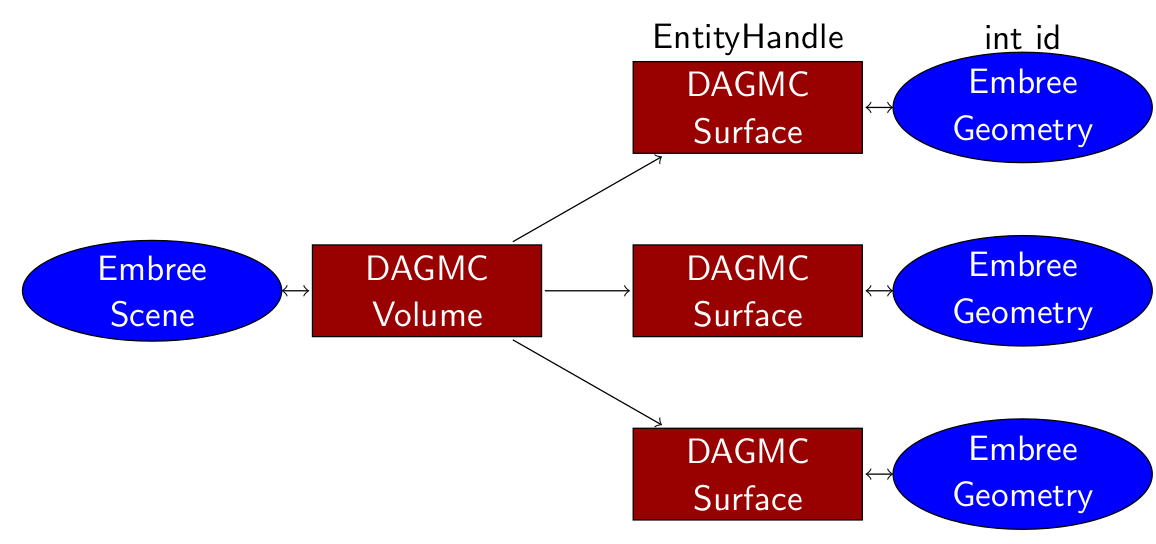
\includegraphics[scale=0.3]{emdag_mapping.png}
  \caption{Representation of MOAB tracking topological connections while mapped to Embree to perform ray queries.}
  \label{emdag_mapping}
\end{figure}

The representation of triangle normals are important to the DAGMC particle
tracking algorithm established by Smith et. al. in 2011 \cite{Smith_2011}. In
DAGMC, particles on or just outside the surface of a volume are handled by
ignoring the near-surface intersection upon being established in a new
volume. This is done to maintain tracking of particles based on their logical
position in the model rather than solely their numerical position which can
cause ambiguities regarding point containment and cause lost particles or
trapped particles between surfaces with infinite histories. Logical particle
tracking is implemented using the convention that triangle normals will always
point outward from the center of the volume they belong to. Triangles hit by the
ray are ignored if the normal of the triangle opposes the ray direction via a
dot product calculation to ensure only exiting ray intersections are
considered. While this has historically been handled inside of DAGMC, this is
accomplished in EmDAG via the use of Embree's filter functions. Filter functions
allow for a user-defined callback method which allows users to validate a ray
hit inside of Embree before returning a final result. Embree will return its
most recent intersection with the scene to the filter function (the hit
triangle's unnormalized vector included) and allow a method to either accept the
hit or instruct Embree to continute tracing the ray path based on the outcome of
the filter function. In MOAB, triangle normals are set in a global manner and
adjusted using stored information within MOAB based on what volume is being
queried at the moment. This is referred to as the surface's sense with respect
to that volume. Because we are forced to duplicate surfaces in Embree, the
triangle normals are pre-oriented based on this surface's sense for the scene it
is being created in upon initialization of the model within the Embree
instance. This saves steps in gathering this information upon traversal when the
triangle normal is needed to determine a particle's logical position within the
model. Though the connectivity of triangles is duplicated using this approach,
the overall memory footprint of EmDAG after duplicating the DAGMC geometry in
Embree is not much greater thanks to the single precision values for vertex
locations used in Embree which will be addressed in a later section of this
chapter.  By meeting DAGMC's requirements in the areas of topology, watertight
representation, and hit acceptance/rejection based on triangle normals, Embree
provides DagMC with all the information needed to perform geometric operations
required by the various Monte Carlo codes it supports, but in an agnostic manner
to the ray tracing kernel being used.

\subsubsection{EmDAG Performance Testing}%%Status:In Progress%%

Using the same DAGMC-based ray fire test program, the performance of DAGMC's ray
fire ability was compared to that of EmDAG's for three models. These models
include a simple sphere, a notched sphere, and a high aspect ratio cylinder. In
each of these tests, the models are tesselated with an increasingly smaller
faceting tolerance in a higher number of triangles and more complex nature of
the surface mesh in terms of BVH construction and traversal. The faceting
tolerance is defined as the maximum distance between the faceted curve or
surface and the geometric curve or surface which it resolves. 600k rays are then
fired from the center of the volume isotropically using the same random number
seed so that the same set of rays is fired in each ray tracing system.

\begin{figure}[H]
  \begin{center}
    \begin{tabular}{ccc}
      \includegraphics[scale=0.13]{sphere.eps} &
      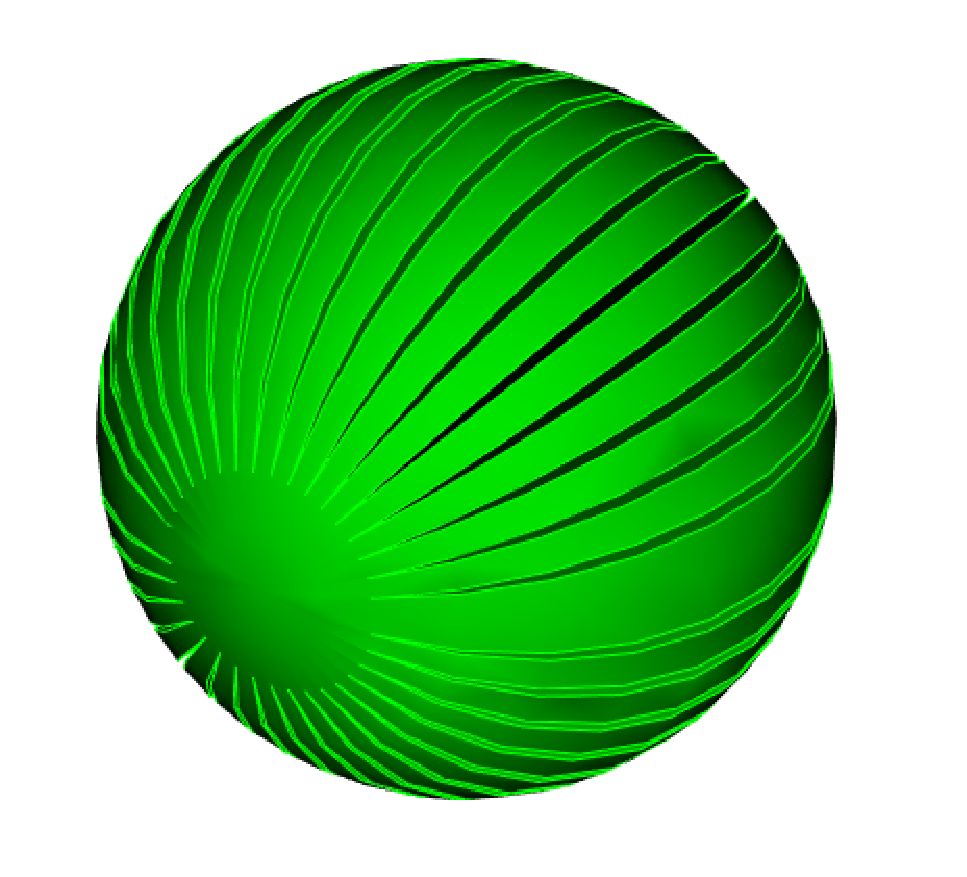
\includegraphics[scale=0.13]{ds.eps} &
      \includegraphics[scale=0.13]{larcyl.eps} \\
    \end{tabular}
    \caption{CAD representations of the sphere, slotted sphere, and high aspect
      ratio cylinder test models used for ray fire timings of DagMC and
      EmDagMC. (left to right) \label{models}}
  \end{center}
\end{figure} 

The sphere and slotted sphere models present speicalized challenges to the BVH
data structure as described in Section \ref{hv_study}. Due to memory contraints
of the system used for testing EmDAG's performance against DAGMC, the ITER
volume was removed and replaced with a high aspect ratio cylinder. The faceting
of the cylinder contains many long, thin triangles running along the barrel of
the cylinder. In similar fashion to the spherical model, the number of these
triangles will increase with decreasing faceting tolerance resulting in an
increasing triangle density as well. The low aspect ratio nature of these
triangles can cause difficulty in the calculations of tightly fitting OBBs
within MOAB's BVH builder. This test model is used to the ray tracing systems
robustness of the BVH generation algorithms to objects with surface meshes of
this nature.

The standard DAGMC ray fire test program (included in appendix A) was used to
evaluate both ray fire systems. The test program itself is agnostic to the
underlying ray tracing kernel used by DAGMC and two versions of the program were
compiled. One in which DAGMC uses MOAB's ray tracer and another in which MOAB's
ray tracing system is subverted by Embree, a.k.a. EmDAG. The two sets of timing
results can be found in Figure \ref{emdag_timing_compare}.

\begin{figure}[H]
  \vspace{-3cm}
  \centering
%  \includegraphics[scale=0.33]{Eig_fix_rf.ps}
%  \includegraphics[scale=0.33]{embree_rf.ps}
  \caption{A comparison of average ray fire times between DAGMC using MOAB's ray
    tracing and Embree. Please note the difference in time scale.}
  \label{emdag_timing_compare}
\end{figure}

Both MOAB and EmDAG scale relatively well for the HAR cylinder model with
decreasing faceting tolerance. This indicates that both systems are capable of
building bounding volumes well for a model with long, skinny triangles. The
scaling of the spherical case with increasing triangles is slightly worse than
the HAR cylinder most likely because the BVH tree is unavoidably going to
becomce gradually deeper as more and more triangles exist in the model. Finally,
the slotted sphere contains many high valence regions and as expected it scales
the worst with decreasing faceting tolerance as the valence of these regions
increases. It is very apparent that there is nearly an order of magnitude
difference in the ray fire timings MOAB and Embree. Due to the very similar
scaling of each test model, it can be stated that the majority of the
descrepancy in the ray fire timings between the two systems occurs in the
traversal methods employed by both systems and isn't likely due to a significant
difference in the structure of the BVH being built by either system. Changes in
the way the BVH is built typically accounts for anywhere from 30-40\% difference
in ray fire timings whereas the descrepancy seen here between MOAB and Embree is
on average \textbf{an order of magnitude better} when using Embree. In large
part, this has to do with Embree's freedom of design without the restriction of
a ray tracing implementation inside the context of another application. MOAB's
flexibility in core design allows for the robust implementation of an oriented
bounding box tree within this context, but comes with the overhead of database
calls to retreieve stored information which can be undesirable for a
high-performance system and doesn't allow MAOB to take advantage of some
implementation optimizations that Embree does. The vectorization of Embree's
traversal through its BVH contributes greatly to its speed. This can be also
considered a part of the design freedom allowed when designing an independent
ray tracing system that cannot not be afforded using only MOAB's database
interface. However, a property unique to MOAB may allow for an implementation
such as this as will be discussed near the end of this work.

\subsection{EmDAG Transport Tests}
\label{subsec:emdag_transport}

As an extension of these pure ray fire tests, the effect of an improved ray
tracing system on particle transport was studied as well. These tests begin with
several simple models and end with the application of EmDAG to one of the models
used for DAGMC performance benchmarking in Chapter \ref{perf_benchmark}, FNG.

The first transport models to be tested were a single cube and single sphere
filled with a dense hydrogen material for high collisionality in the problem
resulting in a large number of ray queries in the transport run. Each of these
models' principal dimension is 10 cm. The source for these models is a 5 MeV
neutron isotropic point source at the center of the volume. One million
particles were simulated in each test. All of the test models were preproccessed
using a faceting tolerance of $10^{-4}$cm. Moving upward in complexity, another
set of tests were run using a set of nested cubes and nested spheres. Each of
the nested volume models contained three cells: the inner volume, a shell
volume, and the graveyard volume. The purpose of these tests was to ensure that
particles could in fact be tracked through multiple volumes robustly. The nested
cubes model contains an extra volume which consists of the original single cube
subtracted from a cube 1cm larger in each dimension. The nested sphere model
contains an extra volume consisting of the original sphere from the single
volume model subtracted from a sphere 1cm larger in radius. As the purpose of
these tests was to test EmDAG's particle tracking between non-zero importance
cells, the dimensions of the offset between the nested volumes is largely
irrelevant so long as particles are in fact reaching all of the cells.

\begin{table}[H]
  \small
  \begin{center}

      \label{timings}
    \begin{tabular}{lccc}

      \toprule
      Test Model & MCNP & DagMCNP & EmDagMCNP \\
      %%\hline
      & \multicolumn{3}{c}{\textbf{time (min)/ ratio to MCNP}} \\
      \hline
      Sphere & 2.93 / 1.00 & 25.13 / 8.58  & 4.73 / 1.61  \\
      Cube & 5.03 / 1.00 & 10.56 / 2.10 & 5.80 / 1.153 \\
      Nested Spheres & 4.35 / 1.00  & 50.82 / 11.68  & 7.94 / 1.83 \\
      Nested Cubes & 4.73 / 1.00 & 9.26 / 1.96 & 4.35 / 0.92 \\
      %%\hline
      &  \multicolumn{3}{c}{\textbf{histories/min}} \\
      \hline
      Sphere & 3.4104E+05  & 3.9944E+04  & 2.1810E+05   \\
      Cube & 1.9879E+05 & 9.4738E+04 & 1.7260E+05 \\
      Nested Spheres & 2.2991E+05 & 1.9877E+04 & 1.3947E+05 \\
      Nested Cubes & 2.1170E+05 & 1.0806E+05 & 2.3026E+05 \\
      \bottomrule
      
    \end{tabular}
  \end{center}
  \caption{Runtime comparison native MCNP, DAG-MCNP, and EmDAG-MCNP over four
    transport test problems.}
  
\end{table}

The native MCNP runs were generally the fastest among the test problems with the
exception of the nested cubes case in which EmDAG-MCNP marginally outperformed
the native code by ~8\%. This is likely due to the fact that very few triangles
are needed to exactly represent the surfaces of cubic volumes. This creates a
very simple problem in the area of BVH building and results in a shallow
tree. The fact that these volumes have multiple surfaces is also of importance
here. MCNP searches linearly through a given cell's (volume's) surfaces to
determine the intersection of a particle with the nearest surface whereas both
DAG-MCNP and EmDAG-MCNP perform this search spatially. In the nested cubes
model, it is likely that the number of surfaces relative to the number of
triangles in their representation is high enough to allow EmDAG-MCNP to overtake
MCNP's CSG calculations. This is a good demonstration of how CSG implementations
suffer from the lack of a spatial search component when creating volumes from
boolean combination of surfaces as mentioned in Section \ref{implicit_surfaces}.

\begin{table}[H]
  \small
  \begin{center}
    \begin{tabular}{lccc}
      \toprule
      Value & MCNP & DagMCNP & EmDagMCNP \\
      \toprule
      %%Hist/min & 2.2991E+05 & 1.9877E+04 & 1.3947E+05 \\
      %%\hline
      \multicolumn{4}{l}{\textbf{Cell 1 Tallies}} \\
      \hline
      Flux  & 5.25725E-03 & 5.25734E-03 & 5.25734E-03 \\
      Energy  & 3.17869E-03 &  3.17873E-03 &  3.17873E-03 \\
      \hline
      \multicolumn{4}{l}{\textbf{Cell 2 Tallies}} \\
      \hline
      Flux  & 1.91645E-04 & 1.91644E-04 & 1.91644E-04 \\
      Energy  & 5.22131E-05 & 5.22137E-05 & 5.22137E-05 \\
      \hline
      \multicolumn{4}{l}{\textbf{Cell 3 Tallies}} \\
      \hline
      Flux  & 1.18371E-05 & 1.18376E-05 & 1.18410E-05 \\
      Energy  & 4.96282E-06 & 4.96285E-06 & 4.96285E-06 \\
      \bottomrule
                        
    \end{tabular}
    \caption{Nested Spheres Tally Results. Flux tally units are
      $cm^{-2}$. Energy tally units are MeV/g. Note: result comparisons of other
      test cases can be found in Appendix B.}
    \label{nestedspheres}
  \end{center}
%%\vspace{-0.2cm}
\end{table}


The results of the single-volume test cases for native MCNP differ slightly from
the agreeing tally results from the DAGMC-based systems. This is not surprising
as DAGMC is known to report slightly different results from native MCNP. As
result comparisons of DAGMC to native codes are not the concern of this study,
only a comparison of the values returned by EmDAG in comparison to DAGMC is
considered. Differences in the tally results between DAG-MCNP and EmDAG-MCNP are
present only in the nested spheres transport model. There is a small difference
in the flux tally for cell 3 as can be seen in Table \ref{nestedspheres}. By
examining the number of particle tracks in each cell, it can be determined that
this discrepancy is caused by a single particle ending in EmDAG-MCNP near a
surface of cell 2 while in DAG-MCNP the particle crosses into cell 3 before
abruptly terminating though it still contributing slightly to the tally in cell
3. It is believed that this difference in tally result is the result of a
systematic difference between Embree and MOAB's ray fire conventionality rather
than Embree's a result of the double to single floating point conversion of the
model that occurs when using EmDAG though this difference in precision is
suspected to be problematic in other ways as was discovered in transport on the
FNG model.

Finally, a full-scale test of EmDAG was conducted on the FNG model using the
same volumetric source as in the performance benchmarking tests described
earlier. Initially this model failed quickly due to lost particles. This was
surprising as the model is expected to have the same watertight fidelity that it
does when using DAGMC. In order to allow the run to complete, the number of
allowed lost particles was increased to the number of the sources particles
being run (1e8). The justification for this allowance being that if the lost
particle rate is small enough, overall performace and results of the run would
still provide a viable comparison of the two systems. In the end, the model lost
255 particles in 100 million histories. While this is concerning in terms of
robustness, the lost particle rate per history wasn't considered high enough
greatly impact the results from a performance comparison standpoint. A timing
comparison of the FNG run using EmDAG-MCNP to the native MCNP model as well as
DAG-MCNP is found in Table \ref{fngemdag}.

\begin{table}[H]
  \small
  \begin{center}
        \begin{tabular}{|c|c|c|c|c|}
      \hline
      \textbf{Implementation} & \textbf{ctme (min)} & \textbf{wall time (min)} & \textbf{ratio} & \textbf{lost} \\
      \hline
      MCNP5 & 209.92 & 205.99 &  1.00 & 0 \\
      \hline
      DAG-MCNP5 & 1023.04 & 1023.05 & 4.99 & 0  \\
      \hline
      DAG-MCNP5 (lt) & 974.99 & 974.75 & 4.73 & 0  \\
      \hline      
      EmDAG-MCNP5 & 303.49 & 303.63 & 1.44 & 255  \\
      \hline
      EmDAG-MCNP5 (lt) & 257.49 & 257.60  & 1.25 & 247 \\
      \hline
    \end{tabular} 
    \caption{A comparison of transport on the FNG model using a 14.1 MeV
      volumetric source over 100M histories for native MCNP, DAG-MCNP, and
      EmDAG-MCNP.}
    \label{fngemdag}
  \end{center}
\end{table}


\begin{figure}
  \centering
  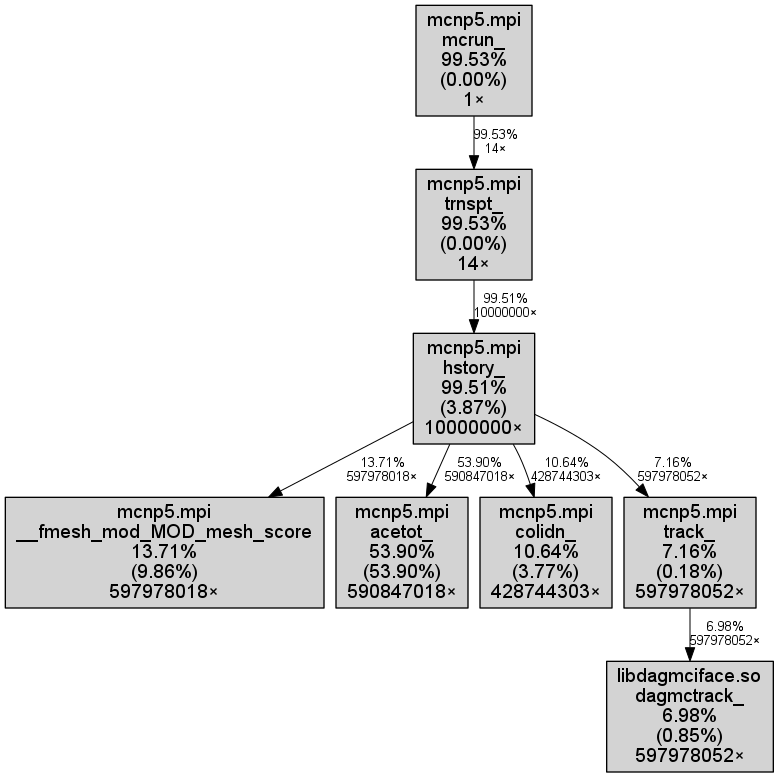
\includegraphics[scale=0.45]{emdag_fng_cg_fine6.png}
  \caption{Callgraph of the EmDAG run on the FNG model for 1E7
    histories. (Processes taking $>=$6\% of the runtime are filtered in order to
    siplify the callgraph.}
  \label{emdag-fng-coarse}  
\end{figure}

While the performance of EmDAG greatly surpases that of DAGMC, it does not come
as close to the performance of native MCNP as it did in the more simple
transport test models. Upon visually inspecting the faceted FNG model, it was
seen to contain many high valence regions. As an artifact of the variance
reduction used in the intended analysis of this model, many planes were inserted
in the model in order to break up large cells with highly varying particle
intensities. Where these planes intersect the cylindrical volumes of the model,
many high valence regions result as can be seen in Figure
\ref{fng-faceted-models}. As a result it became a curiousity as to whether or
not the high valence regions were being handled better by EmDAG than they were
by DAGMC. In order to test this, the same programs used to do the high valence
vertex study were built using EmDAG and the parameter study of the relative high
valence area and valency was performed. The results in Figure \ref{emdaghvstudy}
show that EmDAG also struggles with these high valence regions. In the worst
scenario there is a degradation by two orders of magnitude compared to the best
case scenario which is similar to what seen in the unmodified MOAB ray
tracer. Additionally, it shows degraded performance in the same way that DAGMC
was initally expected to falter - with increasing high valence area and
valency. This is likely due to the nature of the heuristics used by Embree to
construct its acceleration datastuctures.  Unlike MOAB, however, the BVH
building parameters are not as openly available via Embree's interface.There is,
however, an option to reduce the size of the high valence regions in the mode
within the faceting algorithm by definig a length tolerance.

\begin{figure}[H]
  \small
  \begin{center}
    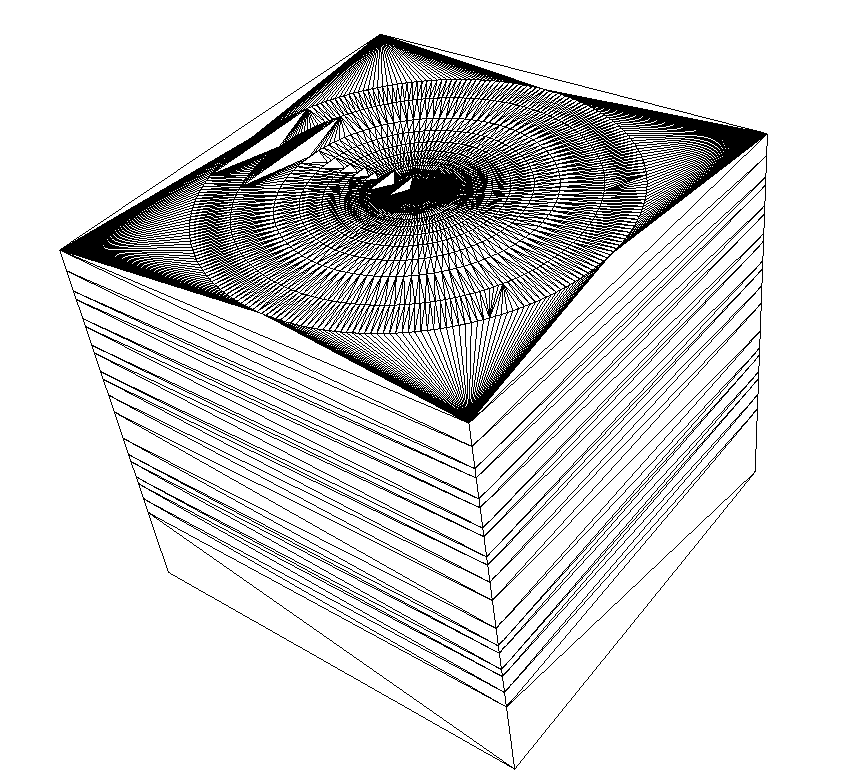
\includegraphics[scale=0.3, trim = 200 0 100 0]{fng_facet_tol.png}
    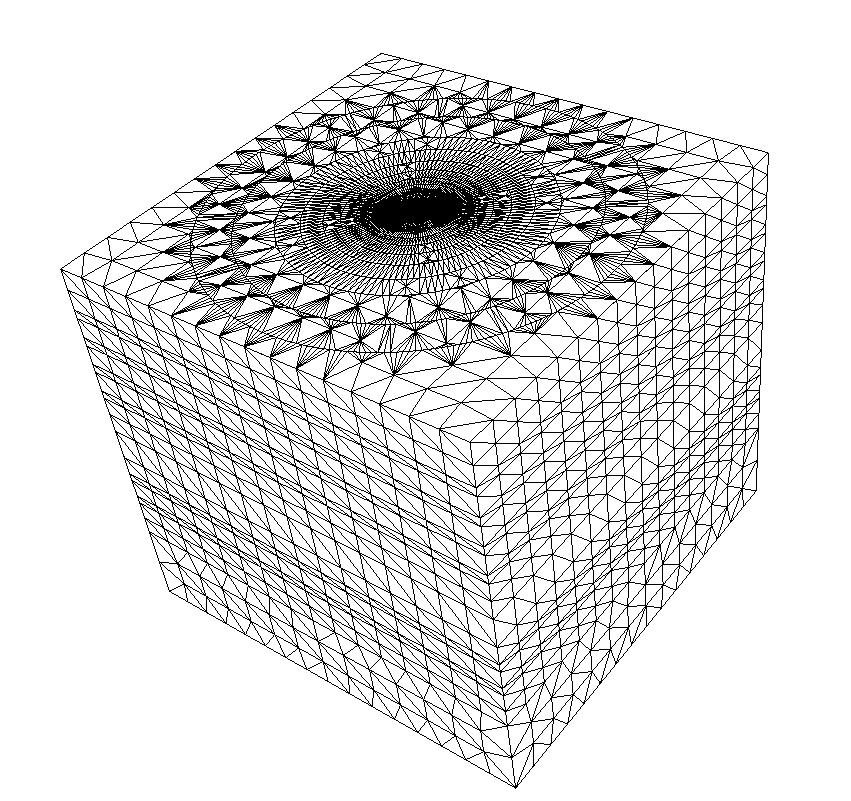
\includegraphics[scale=0.25]{fng_len_tol.png}
    \caption{The FNG faceted model without (left) and with (right) the length
      tolerance applied.}
    \label{fng-faceted-models}
  \end{center}
\end{figure}

The length tolerance is a maximum length for any facet edge returned by the CAD
engine's faceting algorithm. Providing this value to the preprocessing tool
comes at the cost of many more triangles than when supplying only a faceting
tolerance. The difference in facet structure between these models can be seen in
Figure \ref{fng-faceted-models}.

By generating a faceted model using the combination of the length and faceting
tolerances it was hoped that there would be a marked increase in performance
using the EmDAG system and the performance did indeed improve by ~15\%. Due to
the increased number of overall triangles on these planar surfaces, there may be
competing forces at play. As the length tolerance is reduced, the high valence
areas will also be reduced, but the overall number of triangles will increase -
resulting in inherently deeper BVH and longer traversals. Conversely, as the
length tolerance is increased, the number of high valence region areas are
increase, but the number of redundant triangles is reduced improving the average
BVH traversal time enough compensate for a few more rays entering high valence
regions. This observation leads to the idea that length tolerance of the FNG
model could then be optimized. This optimization study, while interesting, will
vary model to model and the results will be complex in nature, depending on the
underlying geometry and geometry adjacent to those regions, etc. In light of the
high valence study results showing that BVH building parameters can be altered
to improve performance and accomodate these high valence regions, it seems that
a better solution is to follow that path over alteration of the mesh globally in
the model. 

\subsubsection{Limitations of the EmDAG system}%%Status:In Progress%%

While the implementation of Embree in DAGMC showed a vast improvement in
performance relative to DAGMC's current implementation, several problems were
encountered during the process. This is not surprising when repurposing a ray
tracing kernal for an unintended application.

One of these problems is the presence of lost particles in a watertight
model. The FNG model EmDAG was tested on is a fully sealed model via the
make\_watertight algorithm. A fully sealed model is one in which every volume is
topologically sealed such that there are no gaps between surfaces or adjacent
volumes. As a result, DAGMC is able to robustly track particles through such a
model with no lost particles. While the lost particle rate for the EmDAG FNG
test relatively low, they in theory should not occur at all as was shown by the
DAGMC runs. After a considerable amount of investigation as to the nature of
these lost particles, their cause was determined to be systematic problem not
encountered in the nested volume cases due to the simple nature of their
geometric topology.

In the DAGMC workflow, a required step for a watertight model is to imprint and
merge the surfaces within the CAD system before faceting the model. Imprinting
is the process by which Trelis, the CAD software used to generate DAGMC models,
makes surfaces and curves that are coincident in space be fully coincident. This
process is accomplished by splitting entities into their coincident and
non-coincident parts. The merging process then topologically combines these
coincident parts into single entities such that the single entities are
topologically adjacent to all entities bounding the original set of entities
that were merged into one. The result of these steps is non-manifold model with
surfaces shared between neighboring volumes \cite{Smith_2011}.

This imprinting and merging of surfaces allows only one representation of each
topological entity to be created upon faceting the model. By using the faceted
curves of the model as a reference for where surfaces meet in space, the
triangles of a surface are then made to meet at those curves in a topologically
watertight manner via the \textit{make\_watertight} algorithm. Topologically
watertight in reference to triangle facets refers to shared connectivity between
surfaces which is distinctly different than watertight by proximity. This
topological watertightness of mesh refers to the fact that triangle surfaces
meshes have connectivity at their interface which share vertex handles inside of
the MOAB database. These vertex handles will then point to the \textbf{exact
  same floating point representation} of the vertices no matter which of the
surfaces is being queried. In this way particles are not lost through gaps in
surfaces and firing a ray from the logcal position inside a volume should always
result in a triangle intersection. This is not the case however when using
EmDAG. Particles were somehow being lost in the transport process.

\begin{figure}[H]
  \centering
  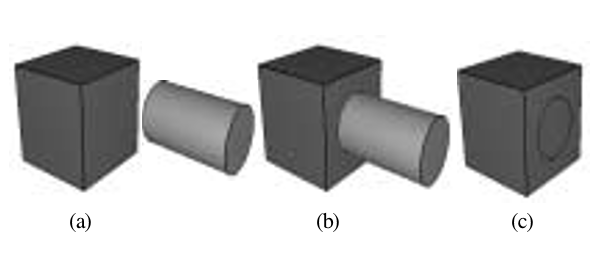
\includegraphics[scale=0.5]{imprint_ex.png}
  \caption{Example of two adjacent volumes being imprinted and merged. a) Two
    volumes, a cube and cylinder are created. b) The cylinder end face is moved
    such that it is coincident with one of the faces of the cube. c) The imprint
    operation is performed and the cylinder curve is imprinted onto the cube
    (cylinder was removed for visibility of imprinted curve). Adapted from
    \cite{White_2002}.}
  \label{imprint_ex}
\end{figure}

Some detailed debugging of this problem revealed that this occurs in a
systematic fashion within the FNG model at intersections of 3 or more
volumes. The secnario is that a particle moves into the intersection between two
surfaces. When this occurs, an intersection with either surface connected to
that interface is a valid hit so long as the surface is part of the volume the
particle is current positioned within. The particle will then logically move
into the volume on the other side of the hit surface. EmDAG handles most of
these cases well but for the case in which a particle will have a zero track
length inside one of the volumes. A zero track length in this case meaning that
the particles trajectory is such that it will only glance a volume without
having any appreciable track length inside of it. In this case, the EmDAG system
may be unable to find a hit whereas DAGMC's tracking is robust enough to find
the triangle intersection on this volume and move on.

\begin{figure}[h!]
  \begin{centering}
    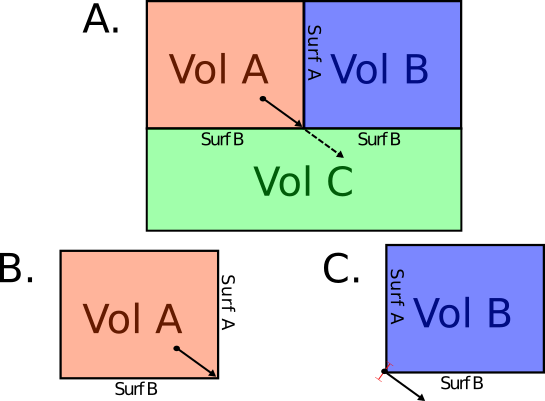
\includegraphics[scale=0.7]{emdag_lost.png}
    \caption{\textbf{A)} The initial scenario of the lost particle. The
      particle's trajectory is such that it intersects with the boundary between
      surfaces A and B. The correct continuation of the particle into volume C
      is depicted as a dashed line. \textbf{B)} An intersection with surface A
      is found though either surface A or B are equally valid. The particles
      position is then updated to its intersection with the boundary of surfaces
      A and B. The particle then logically moves into volume B. \textbf{C)} Upon
      establishment of the particle in volume B the Monte Carlo code requests
      the distance to next surface intersection. The particles position and
      direction are converted from double to single precision. The small change
      in the particle's position places it outside of volume B and the
      trajectory is such that an intersection is not found. At this point the
      particle is considered lost.}
    \label{emdag-lost-particles}
  \end{centering}
  \end{figure}

By isolating this particle's history and producing the particle history with
locations precise enough to detect the descrepancies between EmDAG and DAGMC, it
was found that the position of the particle in EmDAG was numerically too far
outside of a volume to produce the correct triangle hit in either EmDAG or
DAGMC's ray fire systems. The cause of this descrepancy is believed to have to
do with the necessary conversion between double and sinble floating point
precision in the EmDAG system.

As mentioned before, EmDAG uses single floating point representation in its ray
tracing kernel while DAGMC uses a double precision representation of the
geometry and particle information as does MCNP. In order to accomodate Embree's
representation, properties of the particle location and direction are converted
to single precision for ray tracing queries in Embree and back to double
precision when in DAGMC. When changing the floating point representation,
rounding rules based on the computing environment are used to determine the new
representation according to IEEE standards for conversion between precision
levels \cite{IEEE_STD_2008}. These changes in the particle's location and
direction are small, but in the scenario described above it seems that the
particle location and/or direction are altered enough throughout the course of
its history to cause a failed ray intersection - resulting in a lost particle.

In Brandon Smith's thesis, ``Robust Particle Tracking and Advanced Geometry for
Monte Carlo Radiation Transport'' \cite{Smith_2011} there is a detailed
description of the different pathologies encountered in tracking particles
through a surface mesh representation of a geometric model. Briefly mentioned in
this chapter is the possibility of a lost particle due to numerical error in the
particle's position perpindicular to the particle's trajectory. Lost particles
caused by this pathology are not covered however as the double floating point
representation does not allow the particle position to change enough for this
case to occur in practice. In EmDAG, however, this particular pathology is now
vulnerable due to the constant conversion from single to double precision values
between DAGMC and Embree. In order to avoid this problem moving forward, any
improvements to DAGMC's ray tracing kernel for particle tracking will need to
maintain use of double precision representations for mesh elements for robust
coupling of numerical and logical particle positions and directions.


\chapter{High Valence Vertices}\label{ch:high_valence}

High valence vertices are a mesh feature which cause significant degradation in
DAGMC ray tracing performance. The valence of a vertex in a mesh is defined as
the number of edges connected to that vertex. \textit{High} valence vertices are
defined as vertices connected to an unusually large number of edges. This
region, known as a high valence region, will typically take on a fan-like shape
as seen in Figure \ref{fig:hv_examples}.  The geometric origins of high valence
regions are typically a planar surface intersected with some form of curved
boundary condition. 

\begin{figure}[H]
  \centering
  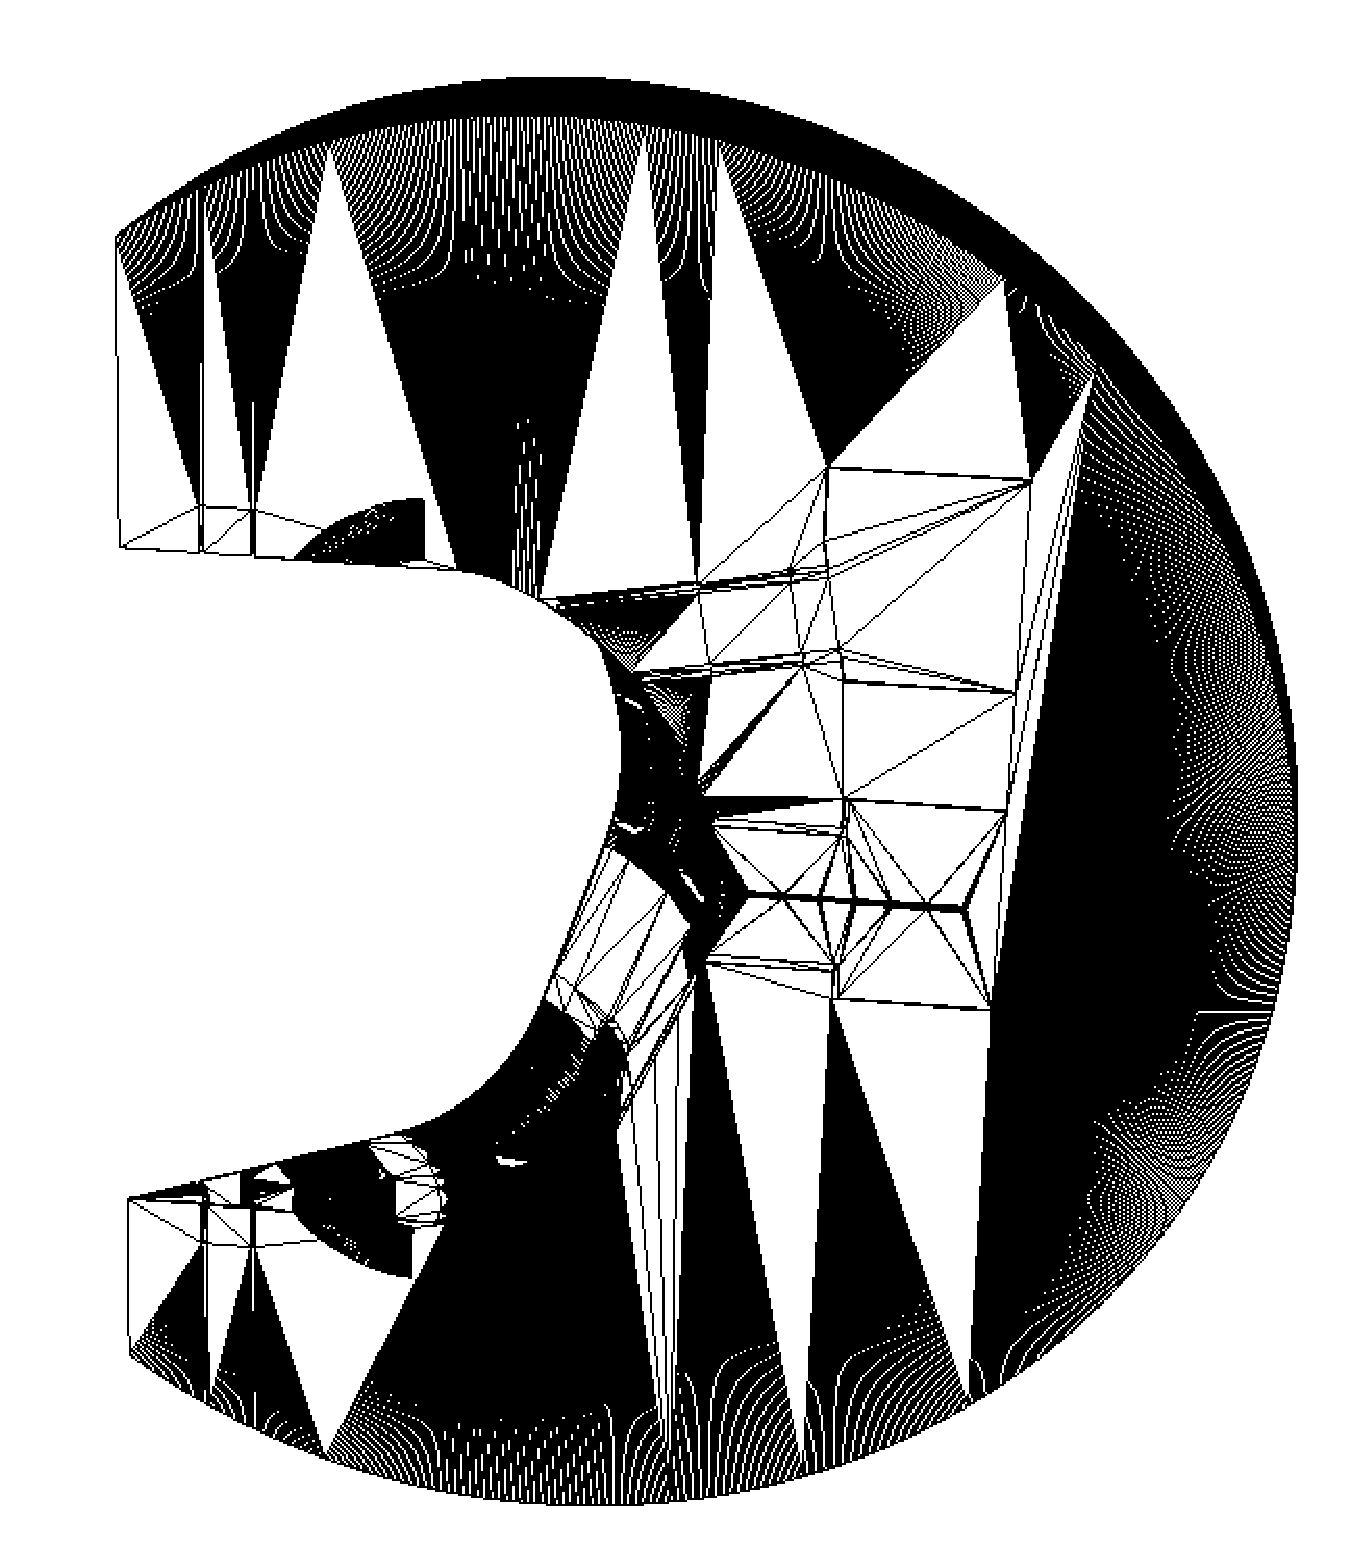
\includegraphics[scale=0.2]{iter_sideon.eps}
  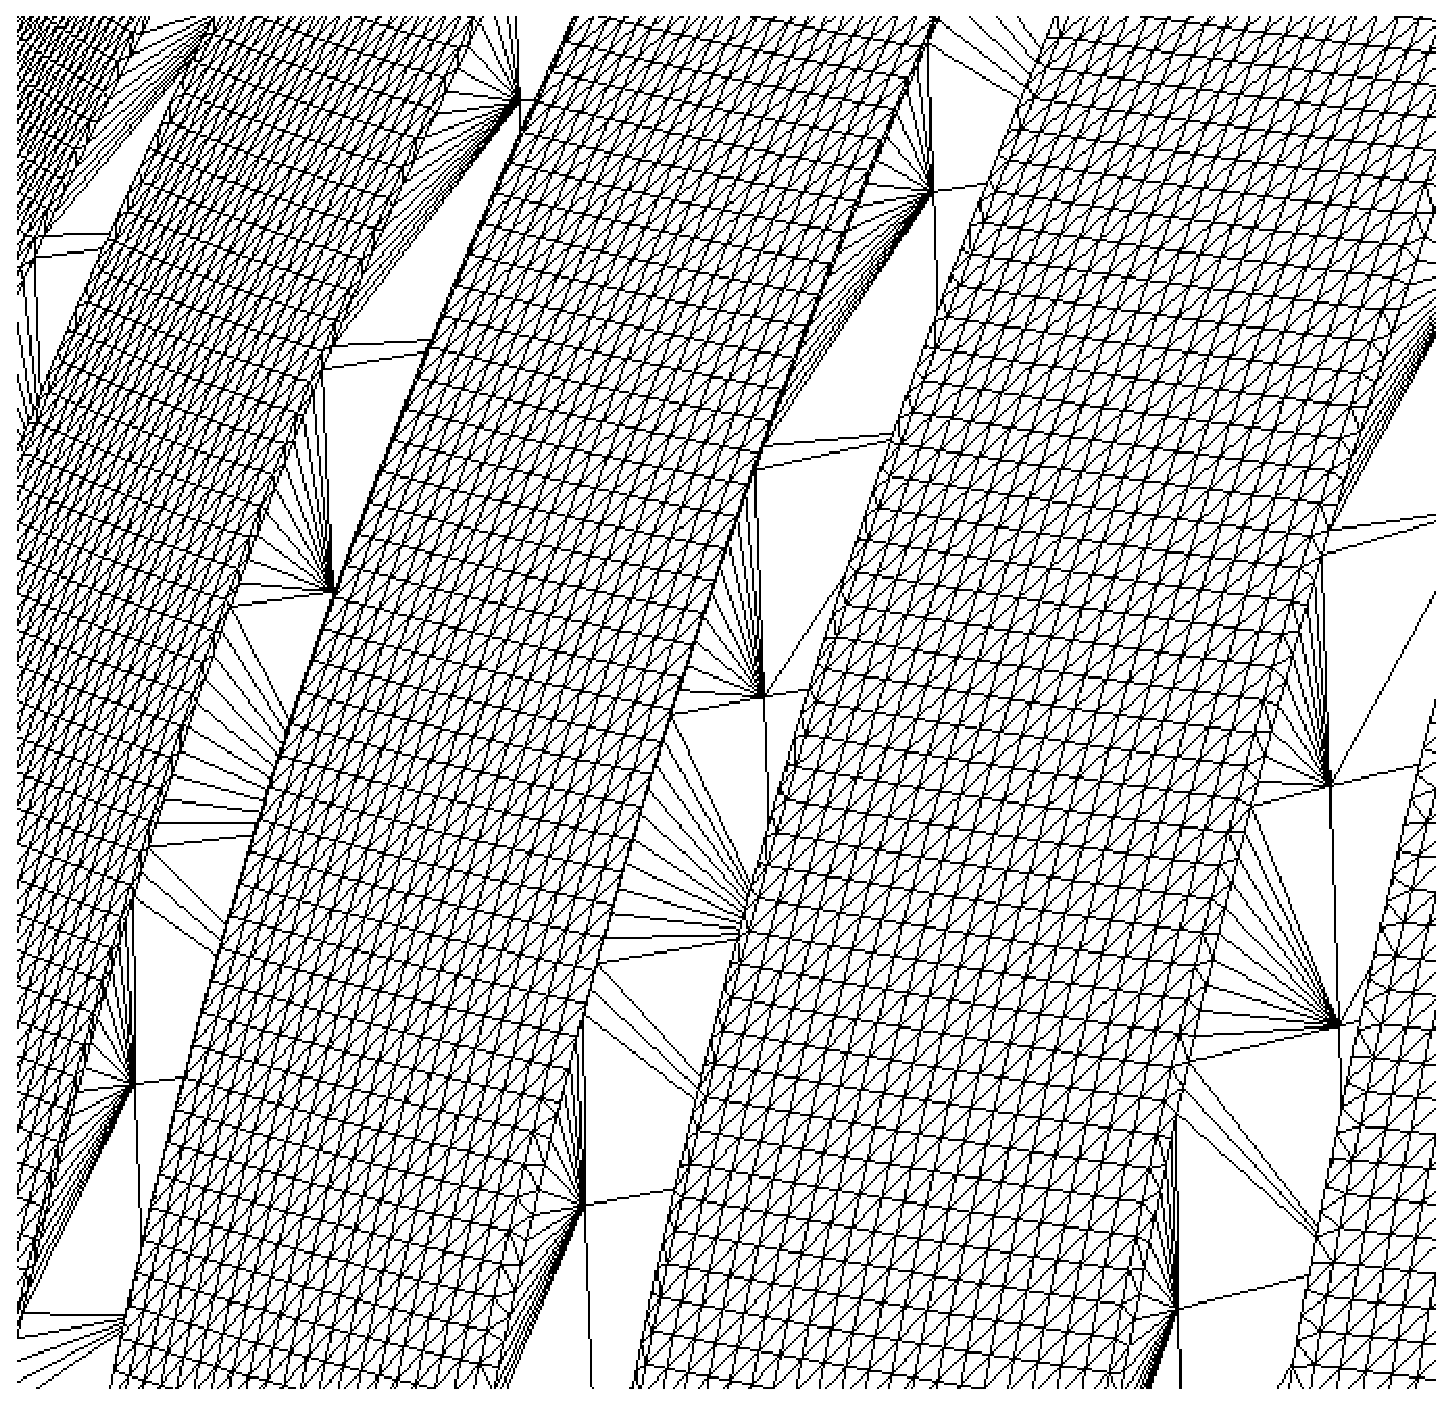
\includegraphics[scale=0.2]{ds_hv.eps}
  \caption{Examples of high valence vertices in analysis and test models.}
  \label{fig:hv_examples}
\end{figure}

These regions are commonly generated in the faceting algorithms used to produce
DAGMC meshes. This faceting scheme (which comes from ACIS libraries underlying
the CUBIT/Trelis graphics engine) is designed to produce the smallest number of
triangles possible to represent the model within the representation tolerance
specified in DAGMC's surface mesh generation preprocessing. This restriction is
favorable to the rasterization process commonly used to display models
interactively in the CAD program. Fewer triangles are better for the purpose
particle tracking in DAGMC as well as long as the geometry is accurately
represented. Even the ideal ray tracing acceleration structure queries for a
given triangle mesh scale as $O(log(N))$, and the size of models being analyzed
using the toolkit provides motivation to keep memory footprints as low as
possible. However, even with fewer triangles undesirable configurations can
impede performance as is shown by a set of tests conducted on models generated
by this faceting scheme.

\section{Previous Work}

A study conducted by Steve Jackson in 2010 on the performance of the MOAB ray
tracer revealed a steep degradation in performance with a decreasing faceting
tolerance or an increasing number of triangles. Using a DAGMC-based ray fire
test program, the performance of DAGMC's ray fire ability was evaluated for four
models. These models include a simple sphere, a notched or slotted sphere, and
an outer volume of an ITER model, shown in Figure \ref{fig:sj_hv_test_models}.

\begin{figure}[H]
  \centering
    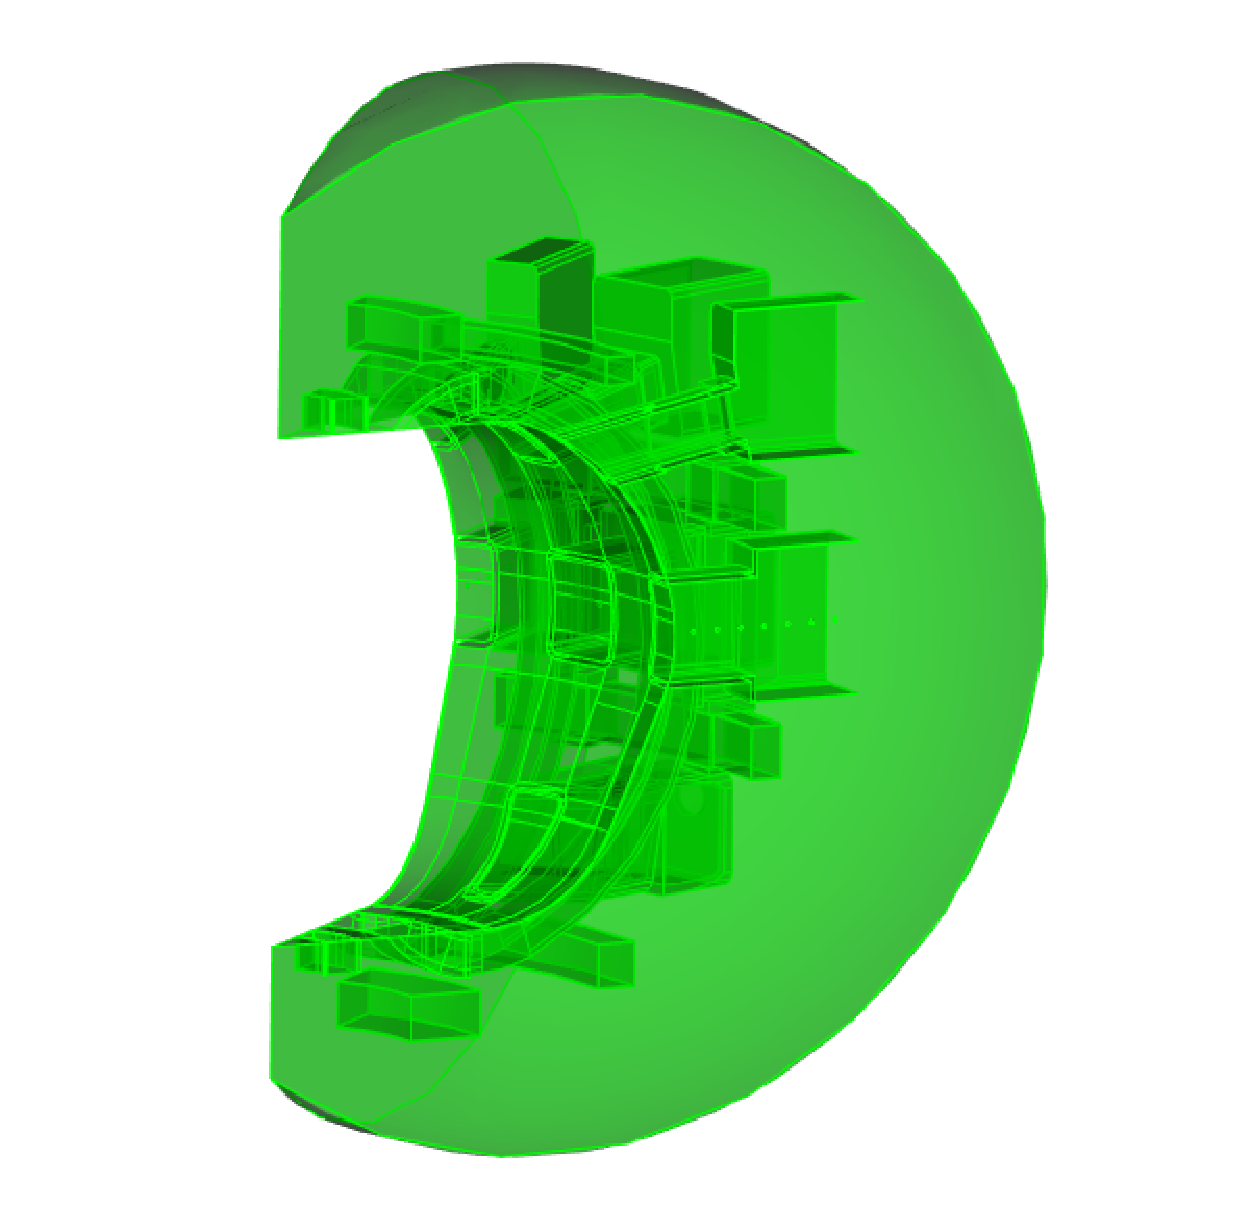
\includegraphics[scale=0.32]{iter_rf_vol.eps}
    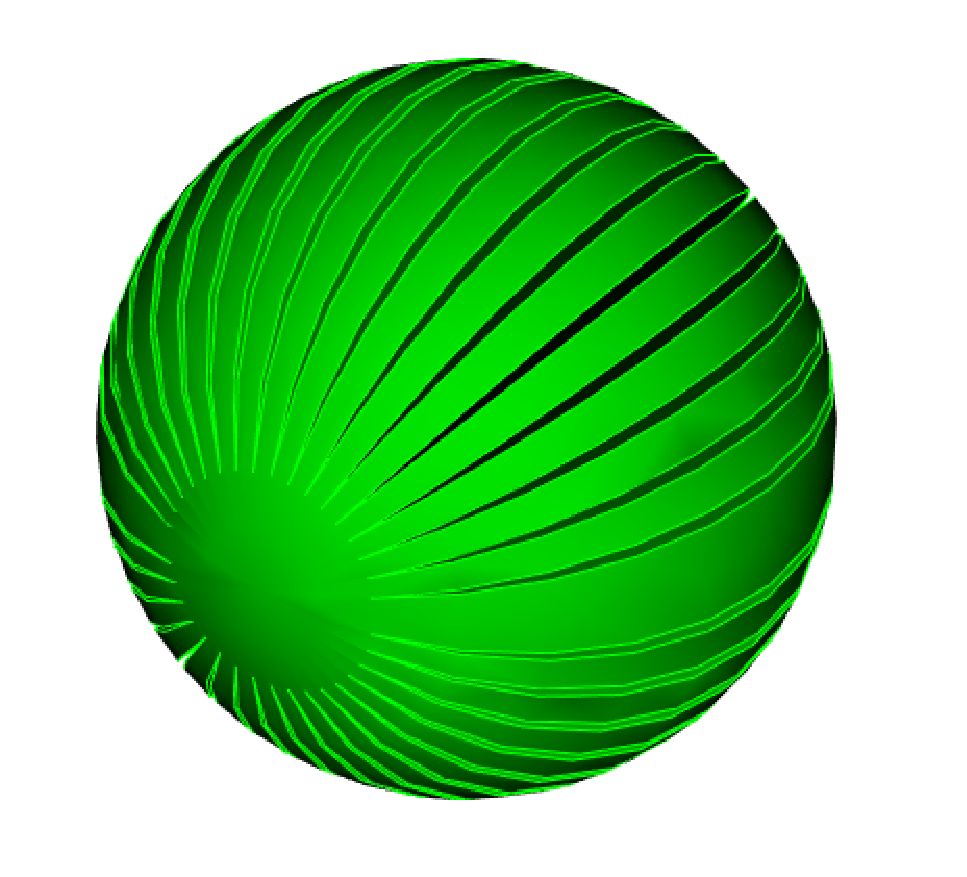
\includegraphics[scale=0.42]{ds.eps}
  \caption{Images of the slotted sphere and ITER volume used to perform DAGMC
    ray fire performance tests with increasing number of triangles or,
    equivalently, decreasing faceting tolerance.}
  \label{fig:sj_hv_test_models}
\end{figure} 

In each of these tests, the models are tessellated with an increasingly smaller
faceting tolerance where the faceting tolerance being defined as the maximum
distance between the faceted curve or surface and the geometric curve or surface
it resolves. By this definition, the number of triangles needed to represent a
model scales inversely with the value of the faceting tolerance. An increase in
the number of triangles leads to a more complex nature of the surface mesh in
terms of BVH construction and traversal.

Each model used in these tests presents its own challenges with increasing
faceting tolerance. The sphere is a good control case for an increasing number
of triangles without change in complexity or exacerbation of pathological mesh
features. The number of triangles generated in the spherical case will tend
toward a maximum value with decreasing faceting tolerance, but the general
nature of the triangulated surface (triangle density, structure, etc.)  will
remain the same. This is not true of geometries with planar surfaces which may
be able to be resolved exactly using some finite number of triangles making the
sphere a valuable test model in that regard. In the case of the notched sphere,
high-valence regions are generated by the faceting engine as a result of its
underlying algorithms for planar surfaces meeting curves surfaces. The high
triangle density of high valence regions causes overlaps in bounding volumes
which become larger as the faceting tolerance decreases. This results in
inefficient hierarchy traversal. Additionally, and perhaps more importantly than
the presence of high valence regions, rays being fired with a point of origin at
the center of the model causes them to travel either exactly along or very near
to the surfaces of the planar slots in the sphere. Such a ray query will visit
many internal nodes of the hierarchy during traversal, creating what is referred
to as a very wide traversal through the BVH as opposed to a narrow traversal in
which fewer branches and fewer nodes of the tree are visited. In this way, the
slotted sphere provides a good measure for the performance of a wide traversal
through the hierarchy in a situation for which many of the internal nodes are
required to be visited. Finally, the faceting of a volume from an ITER model is
used as a production demonstration of the effect of high valence regions on
DAGMC performance (see Figure \ref{fig:hv_examples}).

\begin{figure}[H]
  \centering
  \begin{center}
    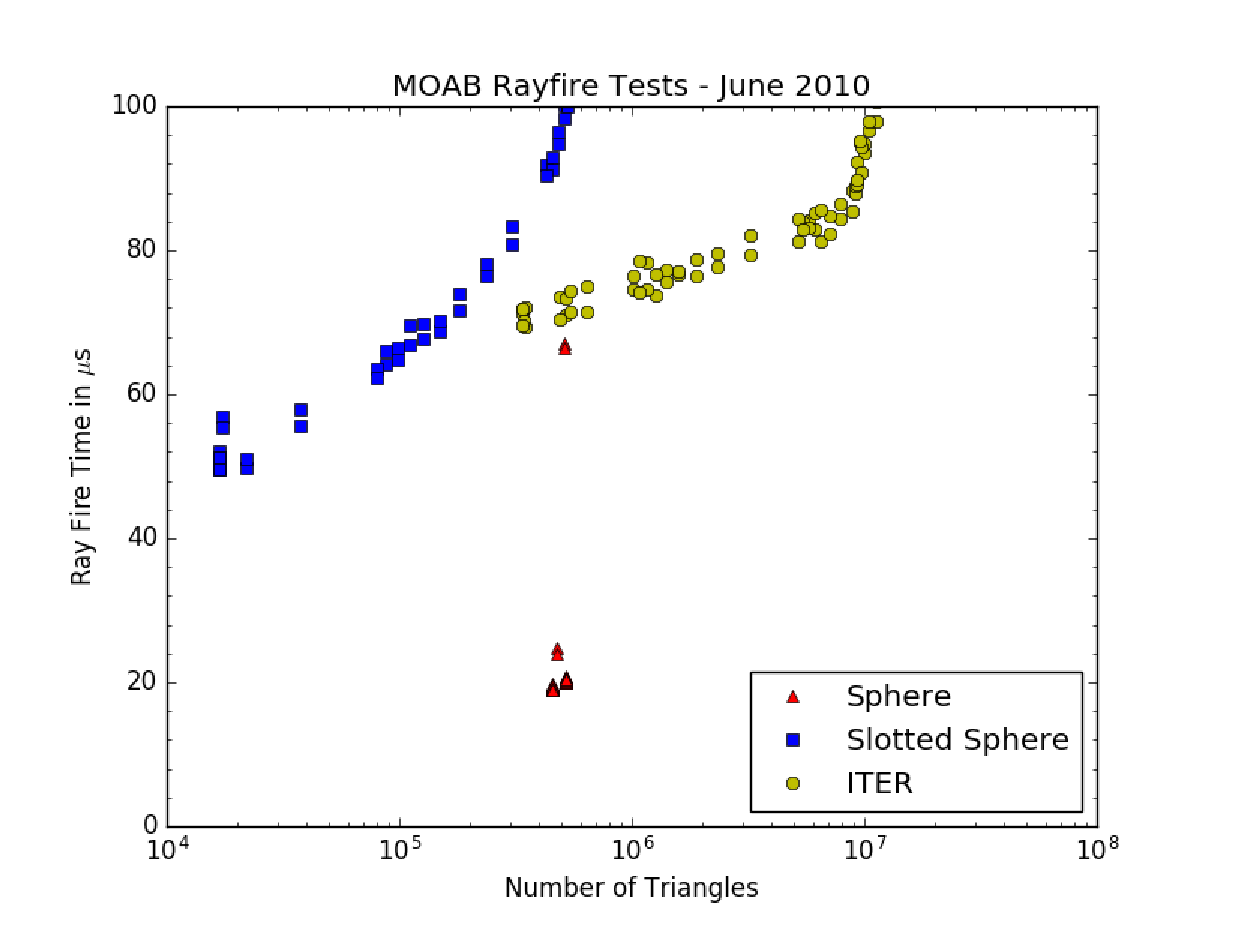
\includegraphics[scale=0.5]{sj_hv_test_results_2010.eps} \\
    \caption{Results of MOAB ray tracing performance tests with decreasing
      faceting tolerance performed by Steve Jackson in June of 2010. Data points
      represent average time spent in firing a ray for random rays
      originating at the center of each model.}
    \label{fig:sj_hv_test_results}
  \end{center}
\end{figure}

While the sphere model scales well with a decreasing faceting tolerance, the
ITER volume and slotted sphere both have a pronounced increase in average ray
fire time with decreasing faceting tolerance. Knowing that both of the latter
models contain high valence regions, it was postulated at the time that these
regions had a significant effect on the scaling.

\begin{sidewaysfigure}
  \centering
  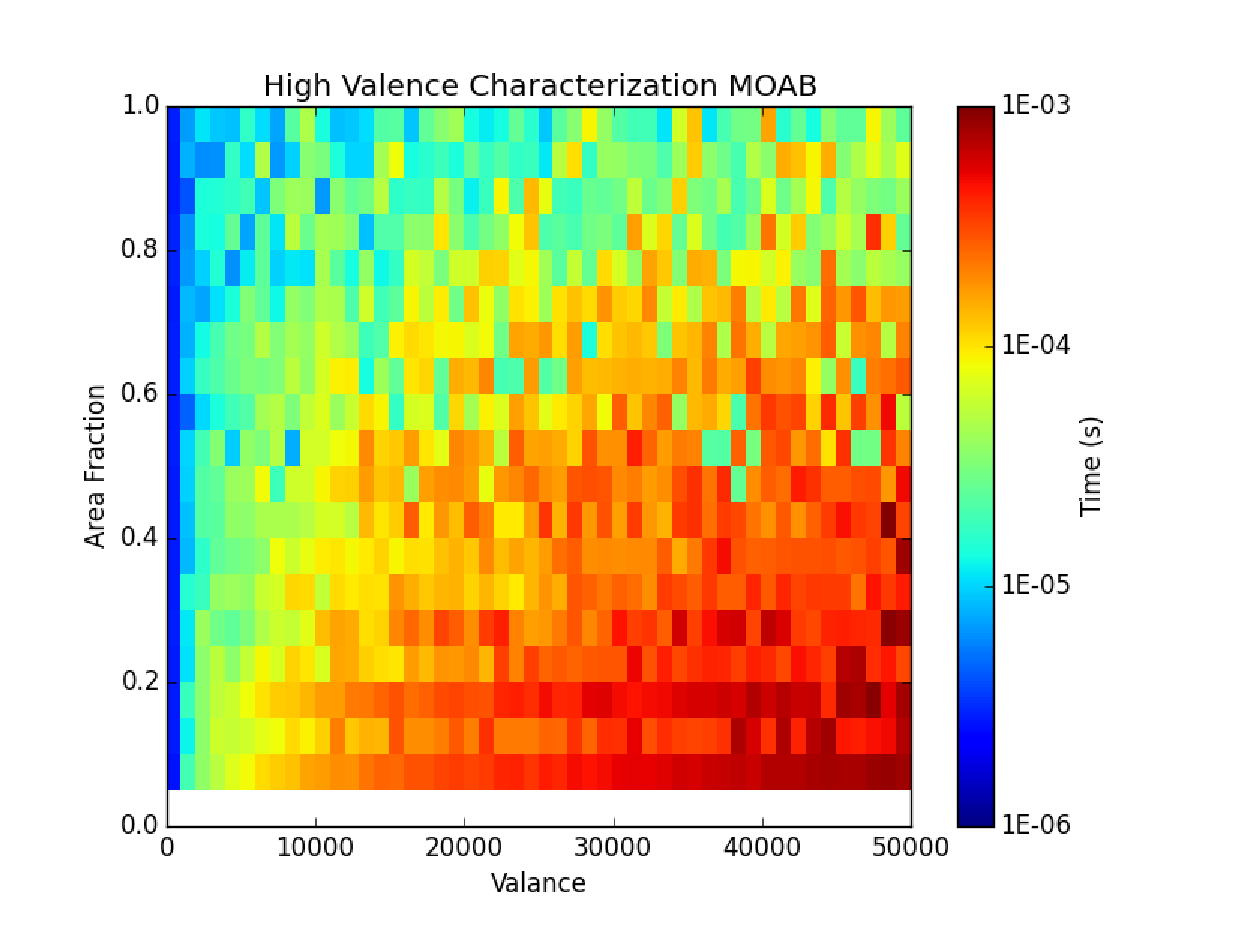
\includegraphics[scale=0.45]{hv_study_MOAB.eps}
  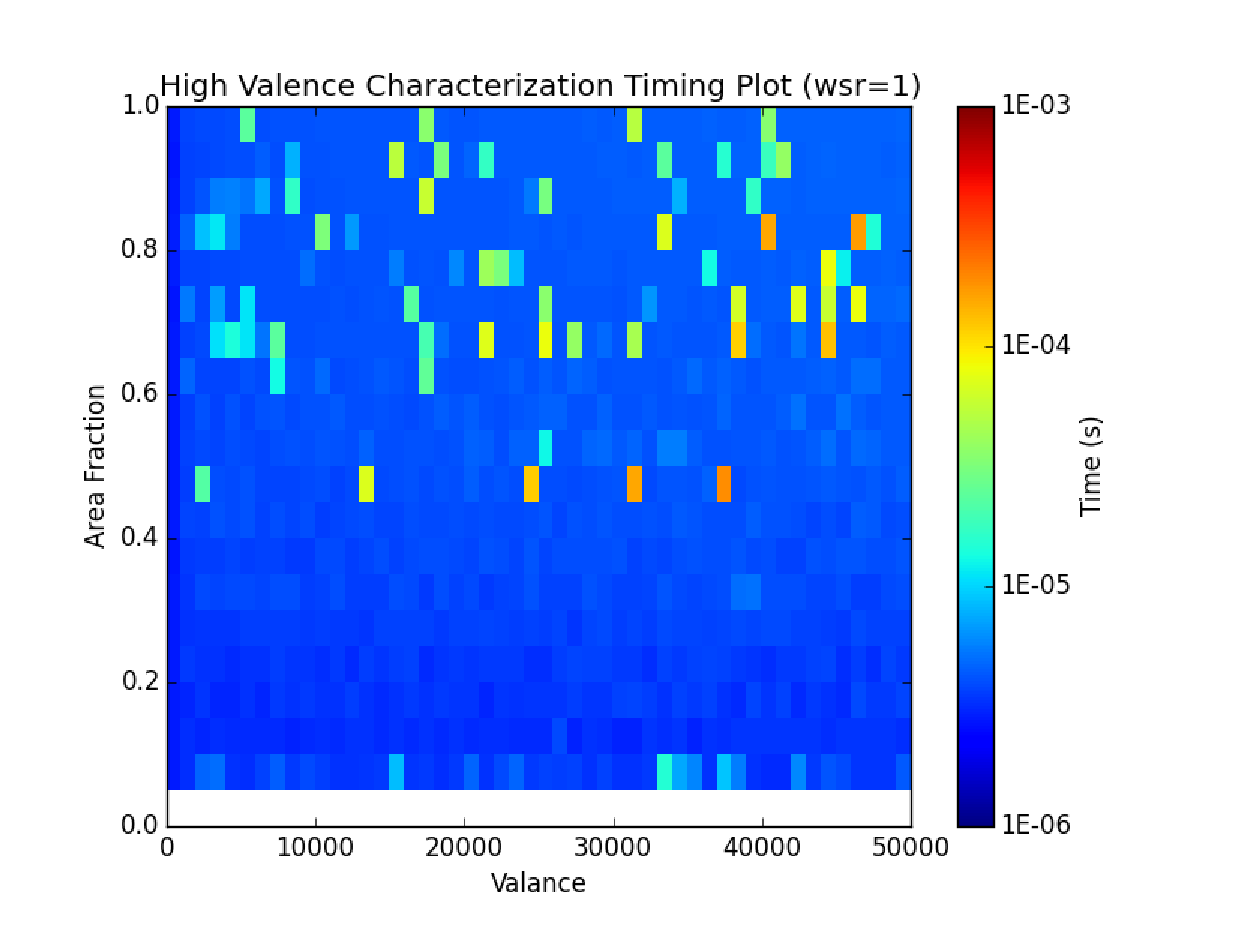
\includegraphics[scale=0.45]{hv_study_MOAB_wsr1.eps}
  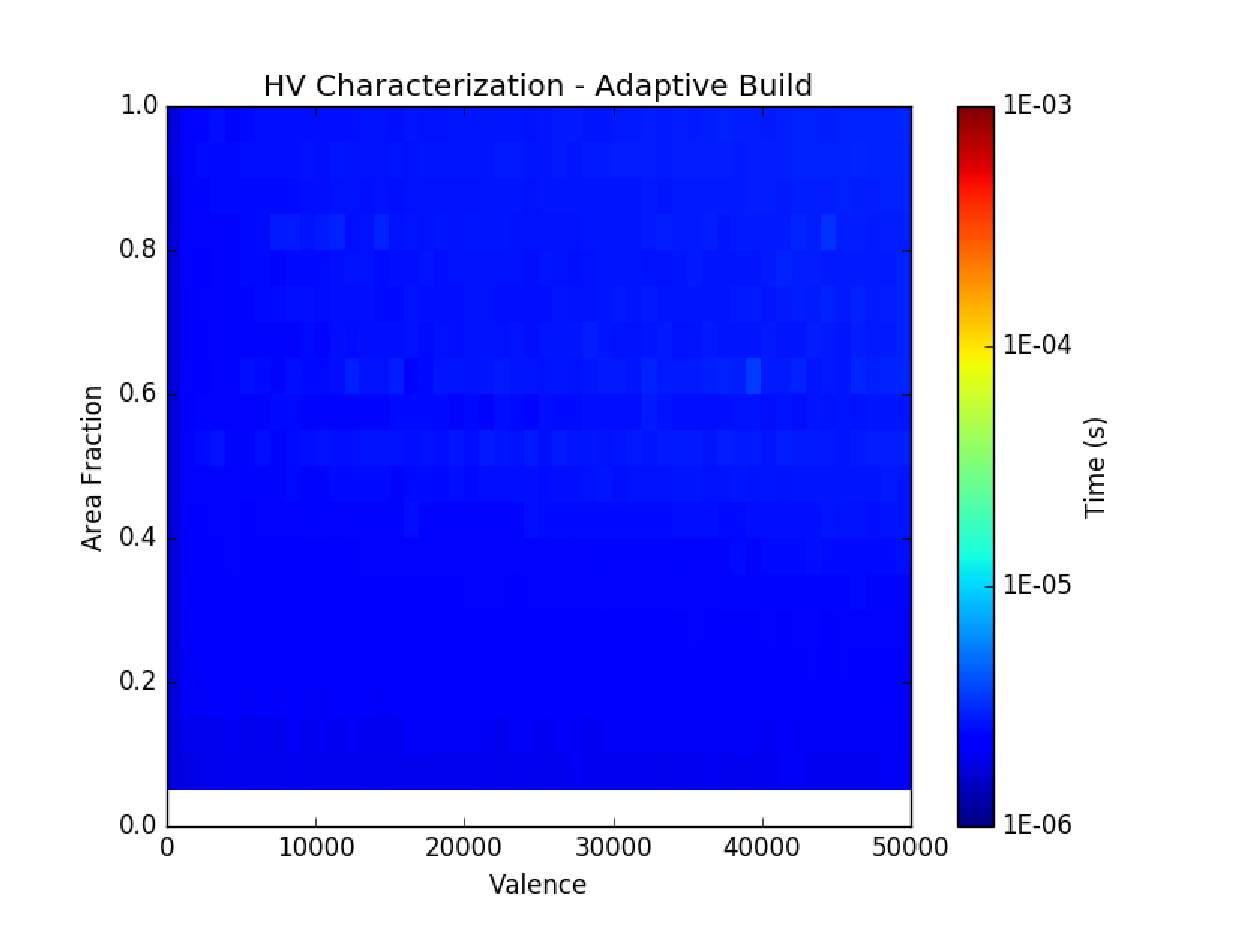
\includegraphics[scale=0.45]{hv_study_moab_adaptive.eps}
  \caption{HV characterization study results for all MOAB OBB tree
    implementations. Top Left: Unmodified MOAB results. Top Right: Maual
    modification of MOAB OBB tree's build settings. Bottom: Results with
    adaptive constrtuction for HV regions.}
  \label{fig:moab_hv_studies}
\end{sidewaysfigure}

\section{High Valence Characterization and Testing Framework}

In order to isolate the high-valence vertex problem generated by the ACIS
graphics faceting algorithm used in Cubit/Trelis, a test model was manually
generated in MOAB with an artificial high-valence region (shown in Figure
\ref{fig:hv_cube_design}). This mesh is a modified cube mesh centered on the
origin in which one of the two-triangle surfaces has been replaced by a more
complex planar surface of triangles including an interior high-valence region
within the face. The high-valence region was generated by inserting vertices
along the diagonal of the interior box and connecting them to the opposing
corners of the box. This mesh is generated using two parameters: the valence of
the corner vertices in the interior region and the relative size of the interior
region. Tests were then performed by varying these two parameters in order to
characterize the performance impediment and determine its root cause.

\begin{figure}[H]
  \centering
    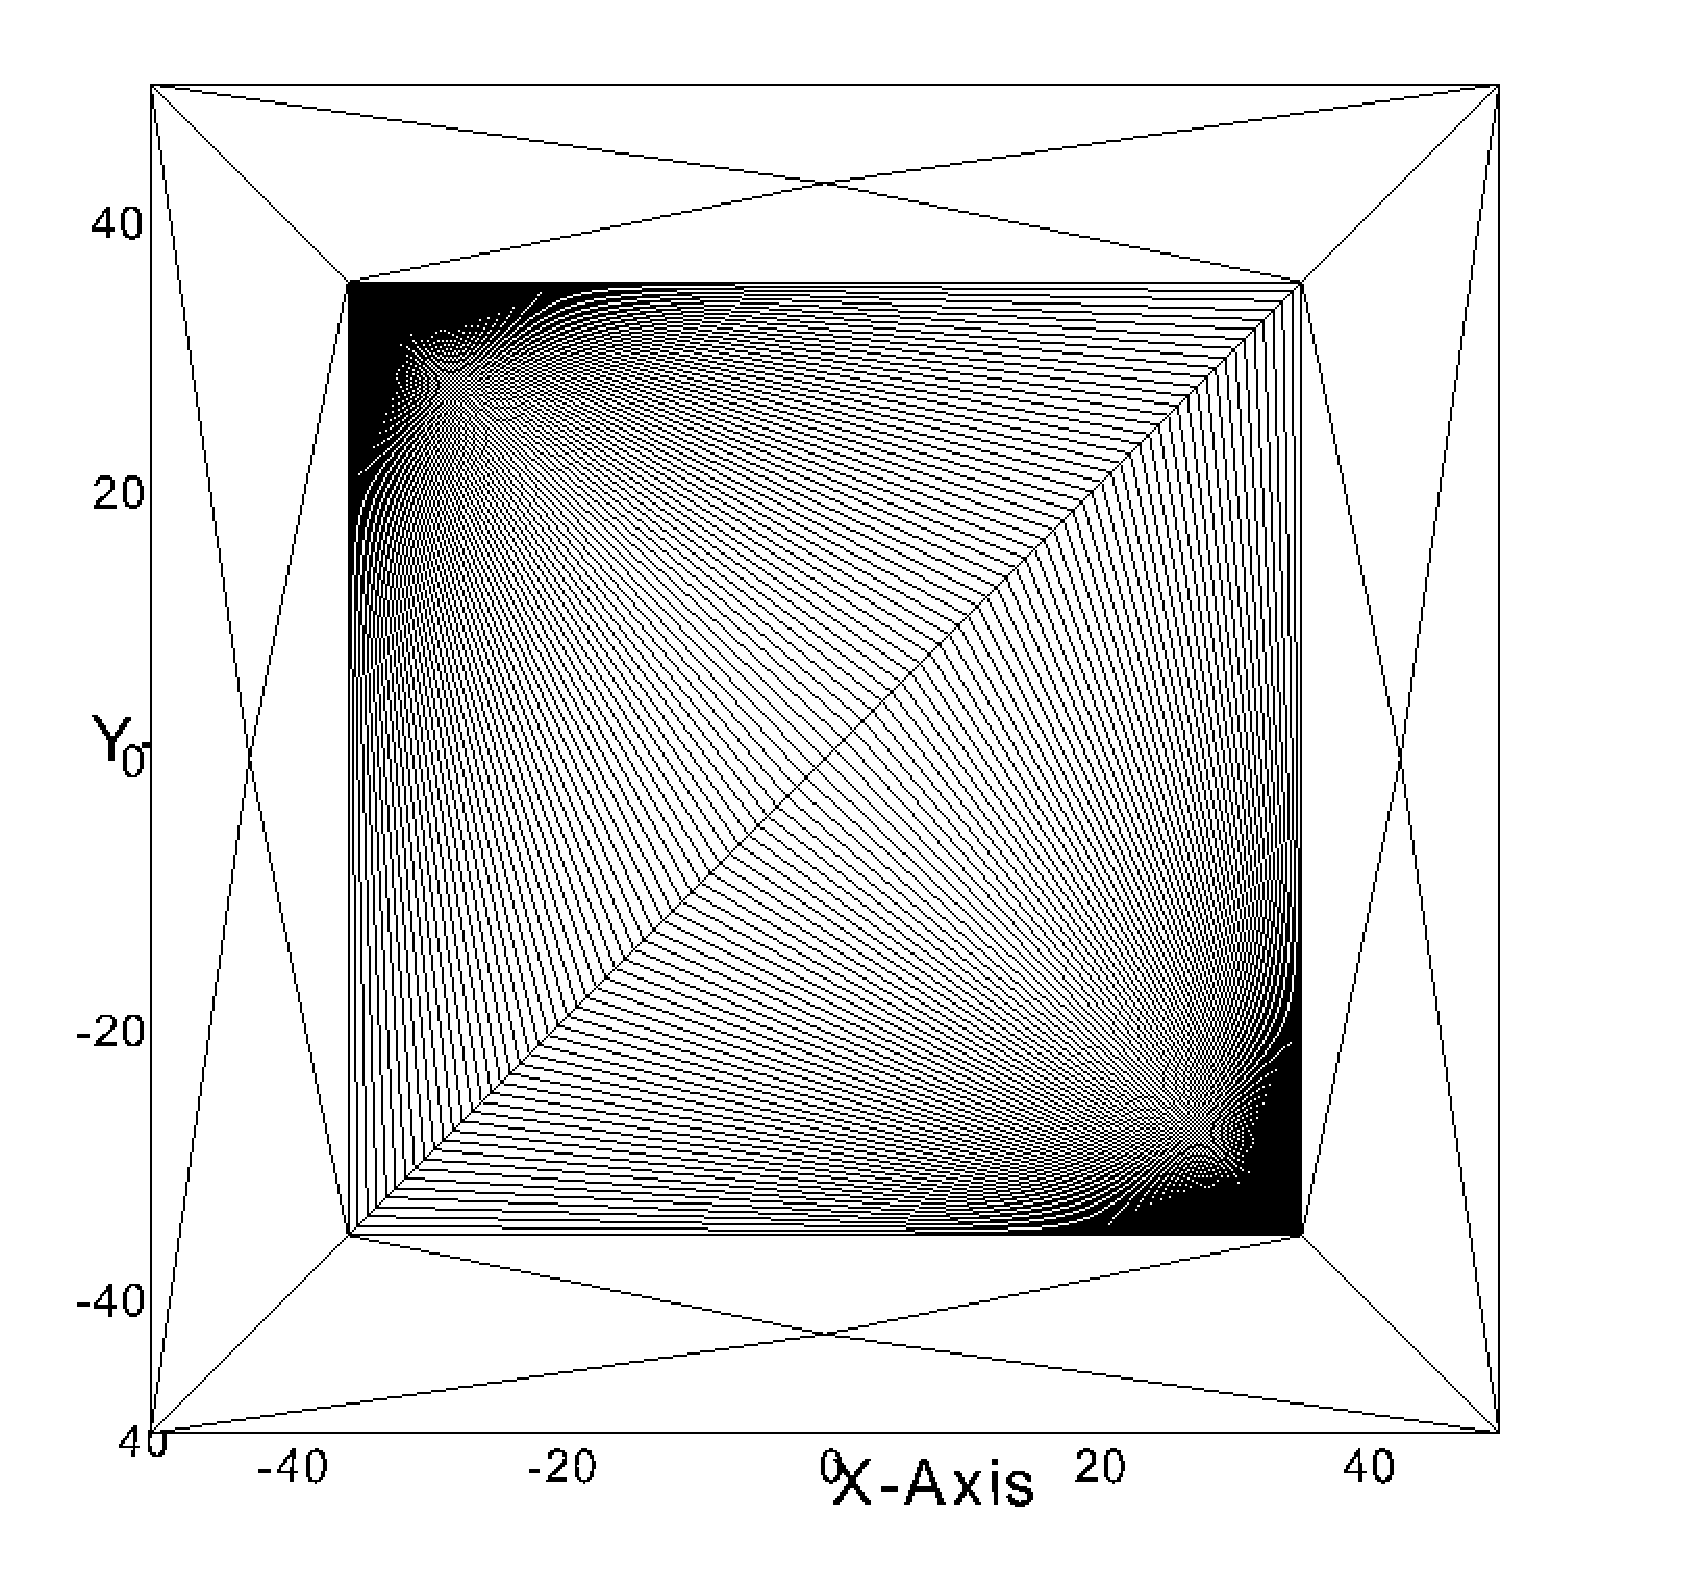
\includegraphics[scale=0.33]{hv_study_design.eps}
    \caption{Side-on view of the modified cube mesh used to study the
      high-valence vertex problem.}
    \label{fig:hv_cube_design}
\end{figure}

A ray fire test program was used to construct MOAB's BVH and perform ray queries
using DAGMC's interface. Information on this test program can be found in the
appendix of this work. This program was used to fire rays with random direction
from the origin of the high valence test model while biasing the ray directions
such that they are always incident upon the modified surface containing the
high-valence region. A parameter sweep was performed by varying the percentage
of the surface covered by the high-valence region as well as the valence of the
region. Specification of the random number seed is allowed within the program to
giving a more direct comparison of performance with the guarantee that the same
set of rays is fired in each test case. Each test shown in this section varies
the valence of the corner vertices from 2 to 50,000 and the relative area of the
high valence region from 0 to 1.

\section{MOAB's Oriented Bounding Box BVH}\label{sec:hv_study_MOAB}

From what is known about the construction of MOAB's BVH, it was expected that
the average ray fire time would be most strongly correlated to the relative area
of the high valence region, but would also increase with increasing valence of
the corner vertices. The initial results of this study, shown in Figure
\ref{fig:moab_hv_studies}, meet only one of the expectations however. The ray fire
times become far worse with increase in valence, but for a constant valence, the
smaller relative area models show a longer average ray fire time than the models
with larger relative areas. This suggests that the presence of a high-valence
region in a surface is detrimental to performance regardless of the likely hood
that a ray intersects with a triangle in that region. In order to investigate
this matter further, a visualization tool for MOAB's BVH was developed to
improve the author's intuition about this mesh pathology.

\subsection{Visualization and Diagnosis}\label{subsec:hv_vis}

Using the same visitor pattern employed to traverse rays through the hierarchy,
each OBB in the HV model tree was converted into a hex element and saved in a
VTK mesh format. Each hex element representing an OBB was tagged with its
depth in the tree as well as the triangle entities it contains, if any. These
mesh files can then be used to visualize the hierarchy level-by-level
superimposed on the geometric mesh. An example of this OBB visualization for the
high valence characterization model is shown in Figure \ref{fig:bad_hv_box}. 

\begin{figure}[H]
  \centering
    \includegraphics[scale=0.3]{{obbs_wsr_0.95}.eps}
    \caption{View of culprit bounding box containing many high valence region
      triangle as well as other surface triangles. Blue box and triangles: leaf
      node bounding box and associated triangles. Several thousand
      triangles are represented in the solid blue region shown here. Red boxes: Other
      representative boxes at the same depth in that tree.}
    \label{fig:bad_hv_box}
\end{figure}

Because there are more entities to partition in the high valence region, it is
expected the lowest levels of the BVH will contain only OBB's bounding triangles
in that region. It was expected that leaf nodes of the BVH might contain many
triangles of the high valence region, causing performance degradation of ray
traversal in that many triangles must be checked for intersection. These types
of poorly formed leaf nodes shift the complexity of the traversal back toward a
linear search - which is sub-optimal. This feature of the produced BVH's in MOAB
were observed, but visualization of the BVH provided the ability to observe
another characteristic as well. Many leaf nodes containing large numbers of
triangles in the high valence region also contained one or two large triangles
outside of that region. The inclusion of these large triangles significantly
increases the probability that a hierarchy traversal will visit that leaf node
and thus all of the triangles contained by that leaf node. This artificial
increase in the high valence regions cross-section greatly exacerbates the
already poorly created nodes in the tree.

Due to the nature of the entity ratio heuristic used to divide nodes in the
tree, as the high valence region becomes smaller more triangle centroids are
shifted onto one side of the median splitting planes used to divide the nodes
which contain portions of that region. If enough triangle centroids are on this
side of the plane, then the cost of the entity ratio evaluation will exceed the
preset upper limit of the cost (0.95 in MOAB) and the construction process will
declare that node a leaf node. This settings governing this split process can be
altered in MOAB, and changing the worst split ratio to 1.0 significantly
improves the average ray fire time in the high valence characterization study,
as seen in Figure \ref{fig:moab_hv_studies}.

As expected, the use of this setting largely removes the degradation in performance
caused by the high valence region by forcing the continued splitting of entities
in the tree where large leaf nodes would have been created before. This
demonstrates that altering this setting works well for this mesh feature, but it
would be detrimental to the memory footprint of the overall hierarchy in the
general case, causing certain areas of the tree to be over-refined. 


\subsection{Adaptive BVH Construction}\label{subsec:adaptive_construction}

One of the benefits to having a BVH tool which is part of a mesh database like
MOAB is the ability to query for more information about the mesh when
constructing hierarchies like the BVH. This information has been used to detect
high valence regions in the mesh and adapt BVH construction to improve the
hierarchy quality in these areas.

\subsubsection{High Valence Detection}\label{subsubsec:hv_detection}

A simple algorithm is used to determine whether or not the entities inside a
leaf node are part of a high valence region. Any vertex connected to more than
$\alpha$\% of the entities in a given leaf node will be considered a high valence
region, indicating that an alternate build method or build settings should be
applied.

\begin{lstlisting}[language=Python,basicstyle=\tiny]
  def detect_hv_region(mesh, entities, alpha):
      assert(a <= 1.0 and a > 0.0)
      connectivity = mesh.get_connectivity(entities)

      to_dim = 2
      for vertex in connectivity:
          # get all entities of dim 2 adjacent to the vertex
          adj_entities = mesh.get_adjacencies(vert, to_dim)

          # determine the number of non-adjacent entities
          overlap = entities - adj_entities

          if( size(overlap)/size(entities) < 1.0 - alpha):
              return true

      return false
\end{lstlisting}

\subsubsection{Implementation}\label{subsec:adaptive_construction_implementation}

First, MOAB's BVH constructor was modified with the option of tagging poorly
formed leaf nodes in the tree. This option will apply a tag to any leaf nodes
which contain more entities the specified in the settings for the tree. These
nodes are then revisited for further refinement later in the build process.

For handling of these poorly formed leaf nodes, a new class was created in MOAB
named the \textit{BVHRefiner}. This class visits each leaf node tagged by the
build process to determine if further refinement is appropriate based on the
available set of mesh features it is capable of handling. For each mesh feature
added to the BVH Refine class, a detection method and build method is
required. This class applies these detection methods and altered build methods
to resolve these leaf nodes into improved regions of the tree. The intent of
this design was to support the detection and adaptation to other pathological mesh
features.

In the high valence case, the refiner class will search for any vertex connected
to more than 80\% of the entities in that particular leaf node. If this condition
is met, the leaf node is declared part of a high valence region and an altered
build method is applied. For the HV case, this build method has been established
by previous work as the standard build algorithm with the worst case splitting
ratio set to 1.0.

\subsubsection{Application to the HV test model}

This adaptive build method was applied to the high valence test model as
before. The results of this test can be seen in Figure
\ref{fig:moab_hv_studies}. Using the adaptive method, the average ray fire
time is consistent across both valence and relative area of the HV region.

\subsubsection{Application in Production}

This method applied to several DAGMC production models in order to determine
its effect on simulation run times during transport.

\begin{table}[H]
  \centering
  \begin{tabular}{c c c c c}
    \toprule
    \textbf{Model} & \textbf{HV Regions} & \textbf{Particle Histories} & \textbf{Runtime reduction} & \textbf{Buildtime increase} \\
    \hline
    FNG            & 514                 & 1M                          & 3.3\%                      & 18.5\%                      \\
    ITER-BLITE     & 3522                & 1M                          & 23.4\%                     & 5.2\%                       \\
    \bottomrule
  \end{tabular}
  \caption{Results of runtime reduction in several DAGMC production models when applying the BVH refinement.}
  \label{tab:bvhrefine_production_results}
\end{table}    

In the case of FNG, the runtime is decreased only marginally, but in the ITER
model the runtime is reduced by nearly $\frac{1}{4}$. It can be presumed that
the reduction in the runtime is associated with the frequency with which a HV
nodes in MOAB's OBB tree are visited. In the FNG model, the HV regions tend to
be smaller and adjacent to the graveyard of the problem while in ITER there are
large HV regions occupying large portions of the external reflecting surfaces of
the model. This provides some anecdotal information about why the refinement has
a larger effect in the ITER model than in the FNG model. It is possible,
however, to quantify this effect more thoroughly by counting the number of HV
node visits in either case during simulation.

\begin{sidewaysfigure}
  \centering
  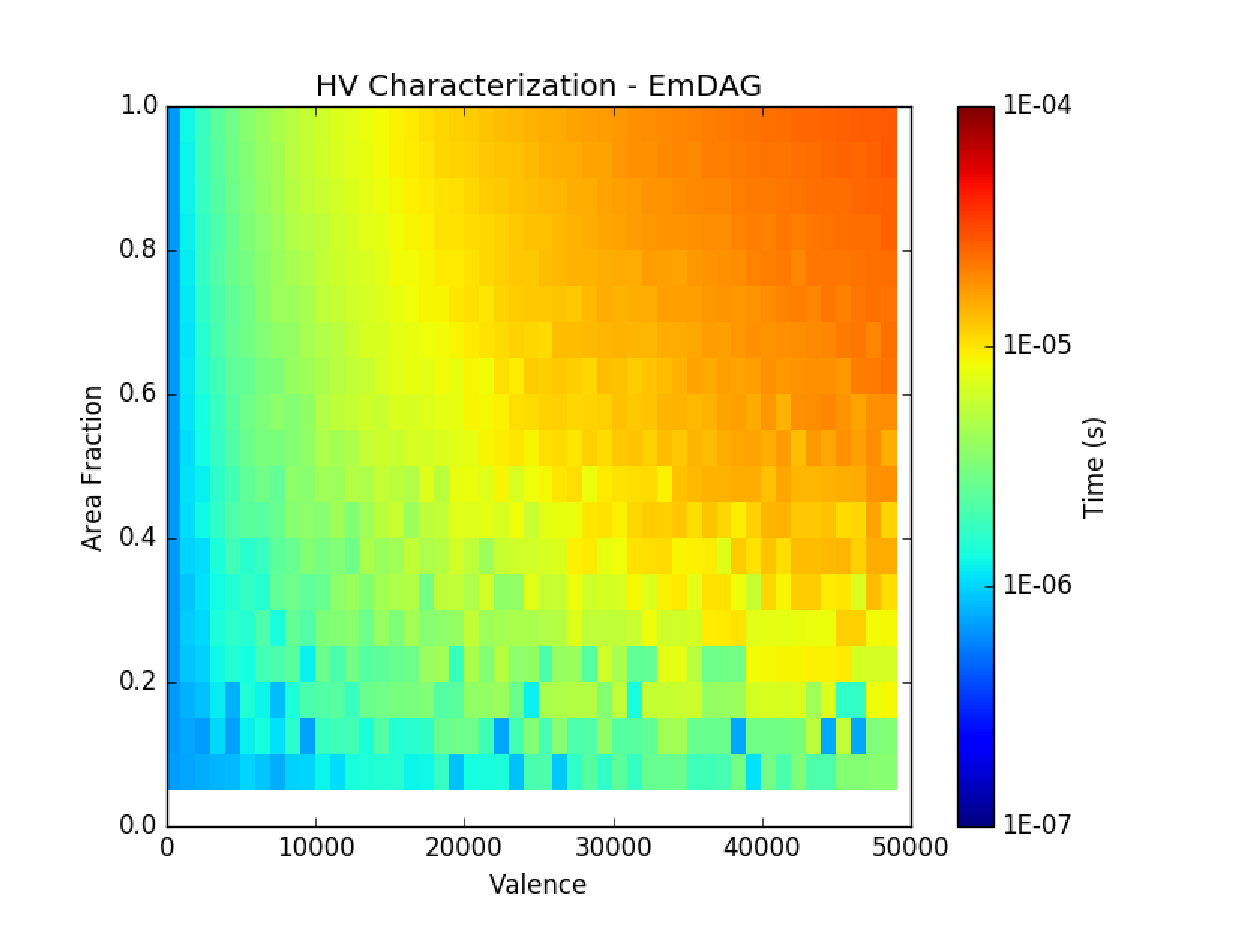
\includegraphics[scale=0.45]{hv_study_emdag.eps}
  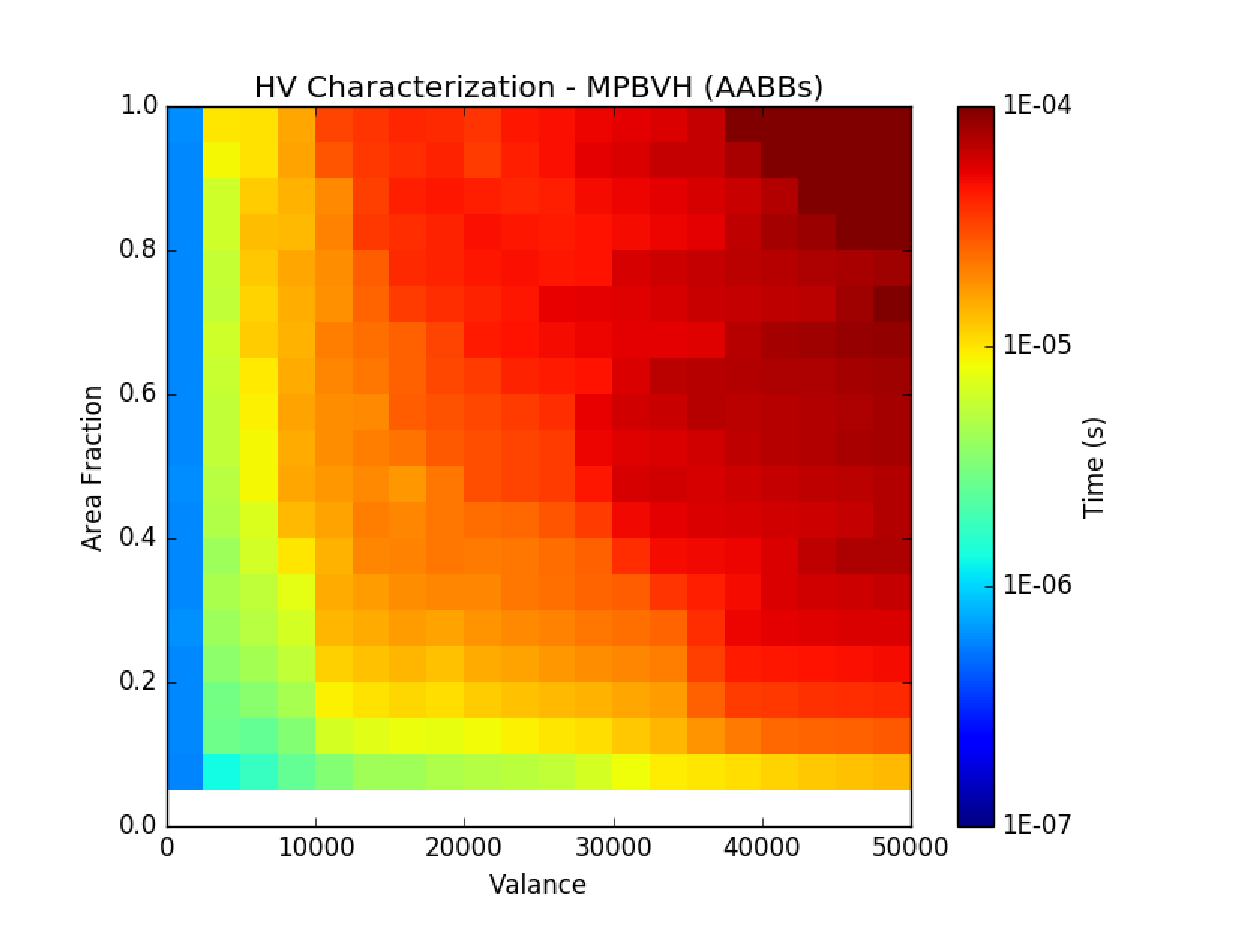
\includegraphics[scale=0.45]{hv_study_SIMD.eps}
  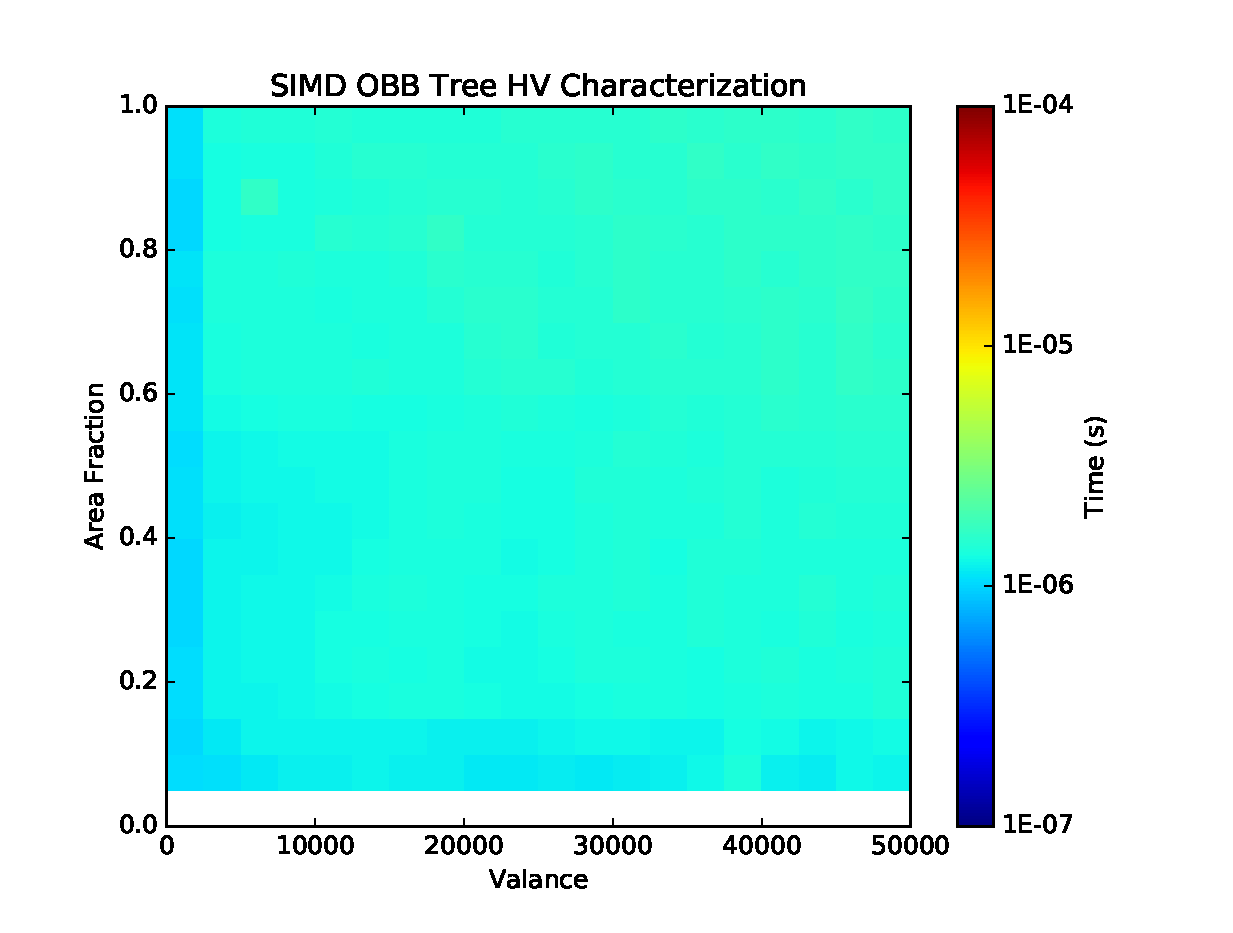
\includegraphics[scale=0.45]{hv_study_SIMD_OBB.eps}
  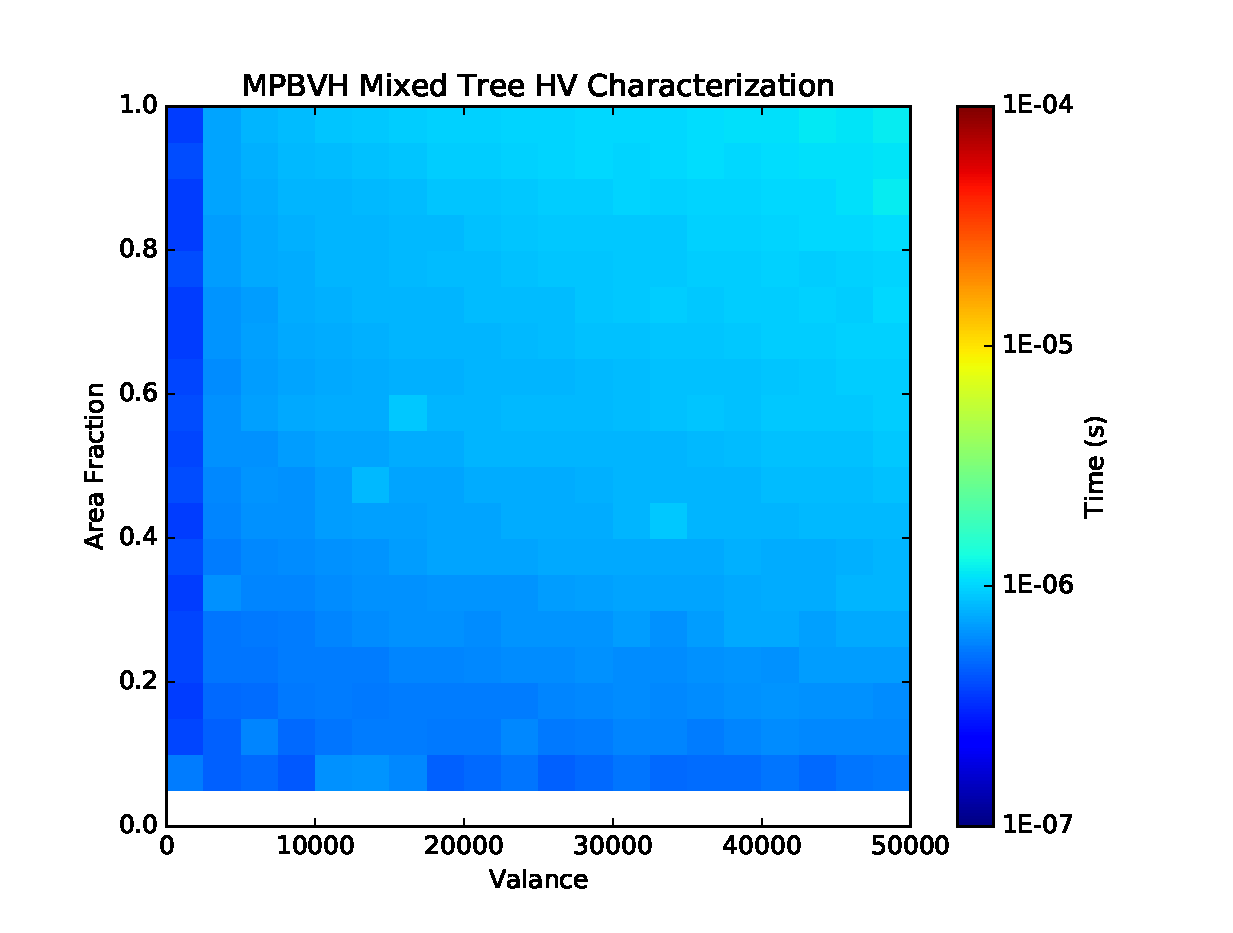
\includegraphics[scale=0.45]{hv_study_mpbvh_mixed.eps}
  \caption{HV characterization results for all SIMD-enabled ray tracing
    kernels. Top Left: Results of the HV study for EmDAG. Top Right: Results of
    the HV study using the MPBVH with AABBs. Botttom Left: Results using the
    MPBVH with OBBS. Bottom Right: Results for the MPBVH with an adaptive build
    method which applys OBBs in HV regions.}
  \label{fig:simd_hv_studies}
\end{sidewaysfigure}

\section{Embree's Ray Tracing Kernel}\label{sec:emdag_hv_study}

Upon visually inspecting the faceted FNG model, it was
seen to contain many high valence regions. As an artifact of the variance
reduction used in the intended analysis of this model, many planes were inserted
in the model in order to break up large cells with highly varying particle
intensities. Where these planes intersect the cylindrical volumes of the model,
many high valence regions result as can be seen in Figure
\ref{fng-faceted-models}. As a result it became a curiosity as to whether or
not the high valence regions were being handled better by EmDAG than they were
by DAGMC. In order to test this, the same programs used to do the high valence
vertex study were built using EmDAG and the parameter study of the relative high
valence area and valency was performed. The results in Section \ref{sec:emdag_hv_study}
show that EmDAG also struggles with these high valence regions. In the worst
scenario there is a degradation by two orders of magnitude compared to the best
case scenario which is similar to what seen in the unmodified MOAB ray
tracer. Additionally, it shows degraded performance in the same way that DAGMC
was initially expected to falter - with increasing high valence area and
valency. This is likely due to the nature of the heuristics used by Embree to
construct its acceleration data structures.  Unlike MOAB, however, the BVH
building parameters are not as openly available via Embree's interface.There is,
however, an option to reduce the size of the high valence regions in the mode
within the faceting algorithm by defining a length tolerance.

\begin{figure}[H]
  \small
  \begin{center}
    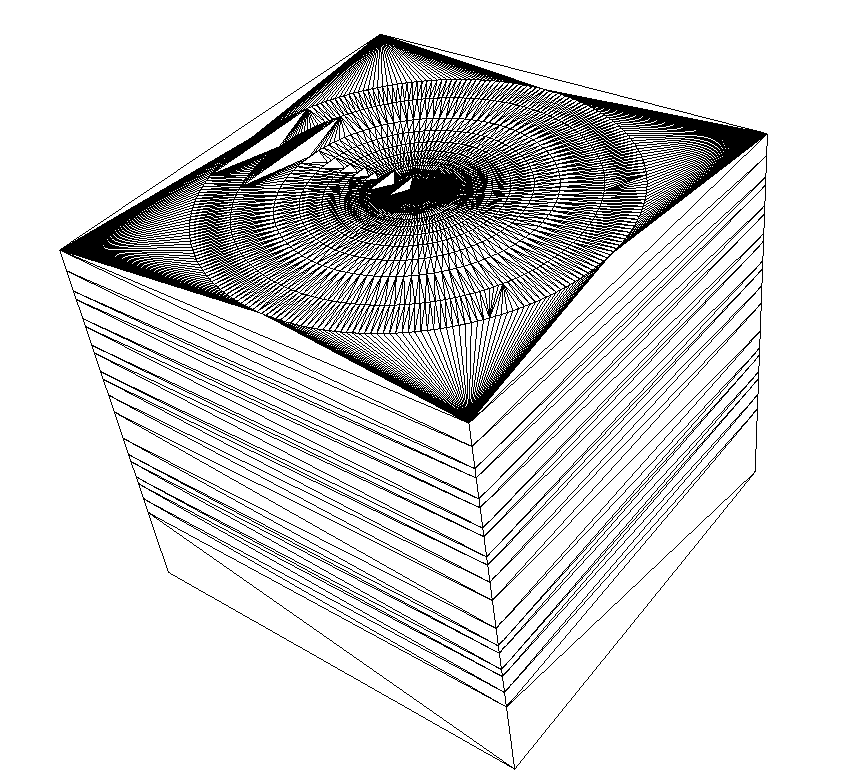
\includegraphics[scale=0.3, trim = 200 0 100 0]{fng_facet_tol.png}
    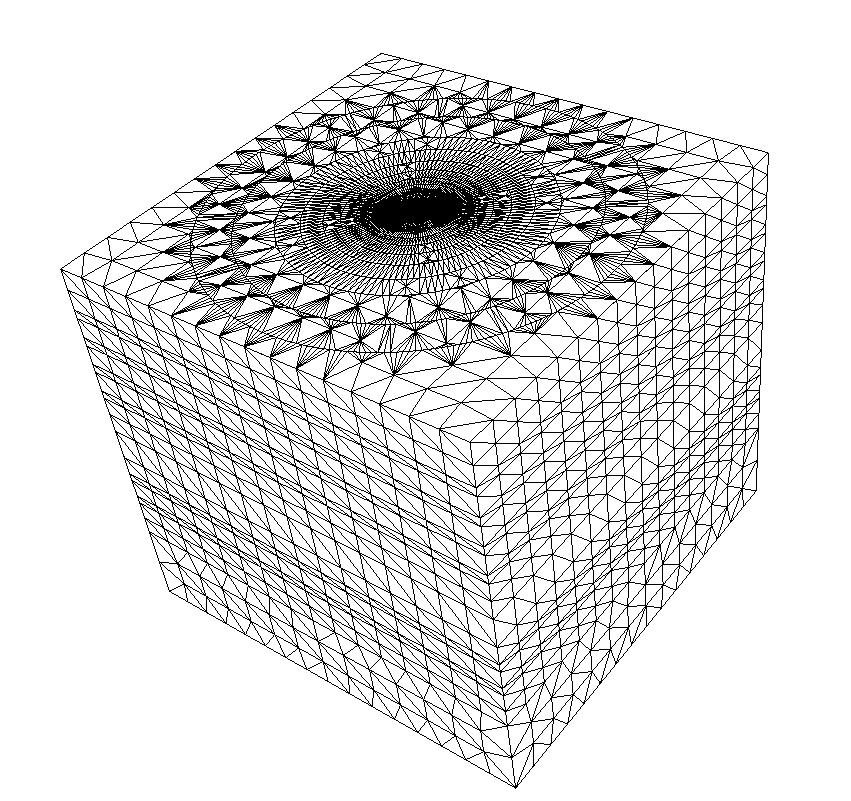
\includegraphics[scale=0.25]{fng_len_tol.png}
    \caption{The FNG faceted model without (left) and with (right) the length
      tolerance applied.}
    \label{fng-faceted-models}
  \end{center}
\end{figure}

The length tolerance is a maximum length for any facet edge returned by the CAD
engine's faceting algorithm. Providing this value to the preprocessing tool
comes at the cost of many more triangles than when supplying only a faceting
tolerance. The difference in facet structure between these models can be seen in
Figure \ref{fng-faceted-models}.

\begin{table}[H]
  \small
  \begin{center}
        \begin{tabular}{|c|c|c|c|c|}
      \hline
      \textbf{Implementation} & \textbf{ctme (min)} & \textbf{wall time (min)} & \textbf{ratio} & \textbf{lost} \\
      \hline
      MCNP5 & 209.92 & 205.99 &  1.00 & 0 \\
      \hline
      DAG-MCNP5 (lt) & 974.99 & 974.75 & 4.73 & 0  \\
      \hline      
      EmDAG-MCNP5 (lt) & 257.49 & 257.60  & 1.25 & 247 \\
      \hline
    \end{tabular} 
    \caption{A comparison of transport on the FNG model using a 14.1 MeV
      volumetric source over 100M histories for native MCNP, DAG-MCNP, and
      EmDAG-MCNP. The DAGMC model was faceted using a length tolerance to
      mitigate the effect of high valence regions.}
    \label{fngemdag}
  \end{center}
\end{table}

By generating a faceted model using the combination of the length and faceting
tolerances it was hoped that there would be a marked increase in performance
using the EmDAG system and the performance did indeed improve by ~15\%. Due to
the increased number of overall triangles on these planar surfaces, there may be
competing forces at play. As the length tolerance is reduced, the high valence
areas will also be reduced, but the overall number of triangles will increase -
resulting in inherently deeper BVH and longer traversals. Conversely, as the
length tolerance is increased, the number of high valence region areas are
increase, but the number of redundant triangles is reduced improving the average
BVH traversal time enough compensate for a few more rays entering high valence
regions. This observation leads to the idea that length tolerance of the FNG
model could then be optimized. This optimization study, while interesting, will
vary model to model and the results will be complex in nature, depending on the
underlying geometry and geometry adjacent to those regions, etc. In light of the
high valence study results indicating that BVH building parameters can be altered
to improve performance and accommodate these high valence regions, it seems that
a better solution is to follow that path over alteration of the mesh globally in
the model.

This study indicates that the simulation improves when faceting with a length
tolerance, but isn't conclusive about the impact of high valence regions on
EmDAG's ray tracing performance. To better understand this impact, a
characterization of EmDAG's reponse for high valence regions was conducted.

\subsection{High Valence Characterization}

The same test described in Section \ref{sec:hv_study_MOAB} was performed
using the ray fire test program compile with using EmDAG to fire rays. A
different behavior was expected when using Embree to construct the underlying
hierarchies due to its use of the SAH. Figure \ref{fig:simd_hv_studies} contains
the results of this test run. Using the Embree kernel, the performance degrades
in direct proportion to both valence and the relative area of the high valence
region. This data represents the expected behavior of MOAB's BVH. Unlike MOAB
however, Embree's use of the surface area heuristic prevents the artificial
increase in probability of visiting triangles in the high valence region. Larger
triangles adjacent to this region are more readily separated from the leaf due
to the additional cost they add by increasing a bounding box's surface area and
in turn its evaluated cost. Separation of triangles in the HV region itself is
still difficult when restricted to axis-aligned candidate split planes.

While this data provides evidence that HV regions are problematic for
production-level ray tracing kernels, it is difficult to employ any adaptive
tree construction techniques. Without access to the underlying mesh
representation of the triangle surface, it is difficult to detect HV regions as
implemented in MOAB's OBBTree. This is both a strength and weakness of Embree's
design in that it can build highly efficient data structures using only
primitive point and connectivity data, but it has no infrastructure in place to
interrogate the mesh more deeply. Methods for detecting and adapting to these HV
regions are addressed using the MMPBVH, a system with similar characteristics
but with more access to the mesh interface. Due to the similarity in design and
use of AABBs, the MPBVH will act as something of a surrogate for the EMDAG in
terms of its response to HV regions.

\section{Mixed Precision Bounding Volume Hierarchy}\label{sec:simd_hv_study}

The MPBVH kernel created by the author has a similar trend to Embree's kernel
where ray fire times increase proportionally to both the valence and size of the
high valence region as seen in Figure \ref{fig:simd_hv_studies}. The author's
BVH applies a modified form of the surface area heuristic in which the surface
area of the box is weighted by the number of entities it contains to determine
if a split is beneficial or not. Near HV regions this heuristic is able to
separate large triangles from the HV region in the same way as the unmodified
surface area heuristic, but it fails to create a well-structured tree for
triangles that are part of the HV area.

\subsection{Visualization and Diagnosis}

Visualization of leaf nodes and the entities they contain for the MPBVH
can be seen in Figure \ref{fig:hv_leaf_simd_bvh}.

\begin{figure}
  \centering
  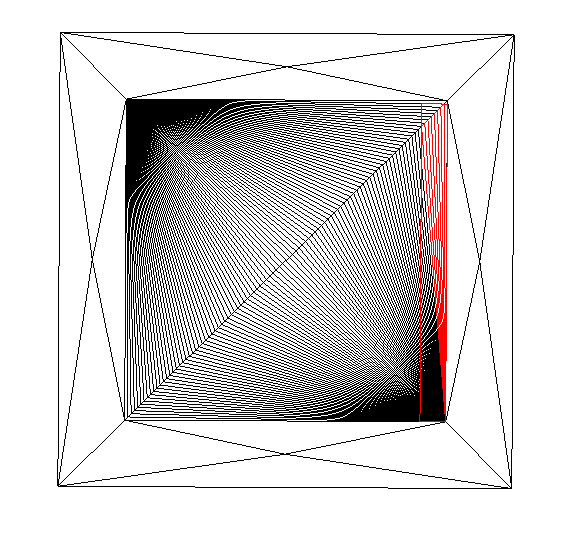
\includegraphics[scale=0.5]{hv_leaf_simd_bvh.png}
  \caption{MPBVH leaf nodes for the HV test model with area fraction
    0.5 and a valence of 100 for the corner vertices.}
  \label{fig:hv_leaf_simd_bvh}
\end{figure}
  
Both Embree and the MOAB SIMD BVH have the shared characteristic of a limited
leaf size of eight primitives due to the way the leaves are encoded. This
removes the possibility that large numbers of triangles in leaf nodes as the
cause of performance degradation, which was true for MOAB's OBB Tree. In the case
of Embree and the MBVH, the largest cause of performance degradation is
overlapping regions of the leaf nodes.

Because both of these implementations use AABBs, bounding of high aspect ratio,
off-axis triangles results in bounding boxes with a considerable amount of empty
space in them. An example of such a leaf can be seen in Figure
\ref{fig:hv_overlap_simd_bvh}. In high valence regions, this results in the same
space being occupied by a high number of leaf bounding boxes. If a ray is fired
into these overlapping leaves, the end result is a large number of leaf nodes,
and in turn, triangles, visited.

\begin{figure}
  \centering
  \begin{subfigure}{.5\textwidth}
    \centering
    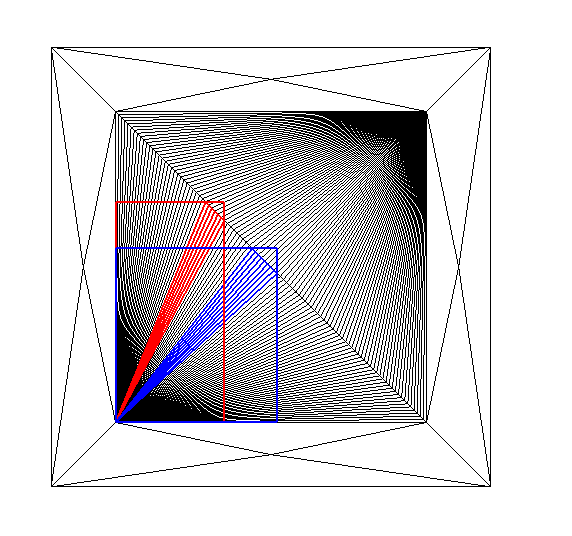
\includegraphics[scale=0.37]{hv_overlap_simd_bvh.png}
  \end{subfigure}%
  \begin{subfigure}{.5\textwidth}
    \centering
    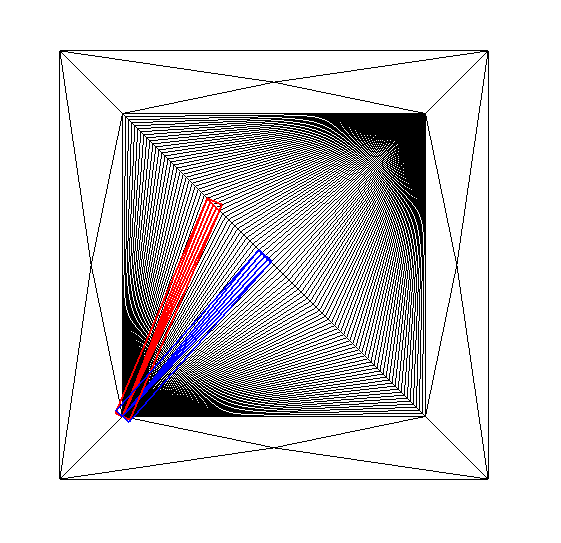
\includegraphics[scale=0.37]{hv_obbs.png}
  \end{subfigure}
  \caption{Visualization of both axis-aligned and oriented boxes surrounding low
    aspect ratio, off-axis triangles.}
  \label{fig:hv_overlap_simd_bvh}
\end{figure}

To alleviate the effect of the overlapping AABBs in this region, OBBs were
implemented as part of the MPBVH. Figure \ref{fig:simd_hv_studies} shows the
results of this study. Because the simplified SAH heuristic is able to separate
large triangles exterior to the HV region into different leaf nodes and the
maximum leaf node size is predetermined, scaling very similar to the MOAB OBB
implementation after HV refinement is applied can be seen, though the overall
speed is somewhat improved due to the single precision implementation.

\subsubsection{OBB Implementation}

The same covariance method used in MOAB to construct OBB's was applied in the
MPBVH \cite{Weghorst_1984}, but the storage technique used differs in order to
accommodate the SIMD programming involved in the BVH traversal. OBB nodes are
stored as scaled, affine transformations of the global problem space and the
box's lower left corner is stored as a scaled reference point. When a ray is
intersected with a node it is transformed and scaled at the same time, but
separately, for each of the four OBBs the node represents. A reciprocal
direction is then calculated with respect to the oriented axes of each
box. Intersection values and distances are then returned in the same way they
are calculated for a node of AABBs \cite{Wald_2014}.

OBB nodes contain additional information in the form of the affine space
transformation and are more computationally expensive when computing ray
transformations. Some of this computational cost is avoided by incorporating the
spatial scaling of the node into both the affine space and reference point to
avoid the additional computational cost of scaling the parametric values of the
ray intersection later in the calculation.

\subsection{OBB Ray Fire Testing}

The tests of the raw ray fire speed using only OBBs were performed using the
MPBVH. The results of these tests can be seen in Figure
\ref{fig:rf_test_results_obbs}. These tests were conducted primarily as
verification that the exclusive use of OBBs results in a slower ray fire times. 

\begin{figure}[H]
  \centering
  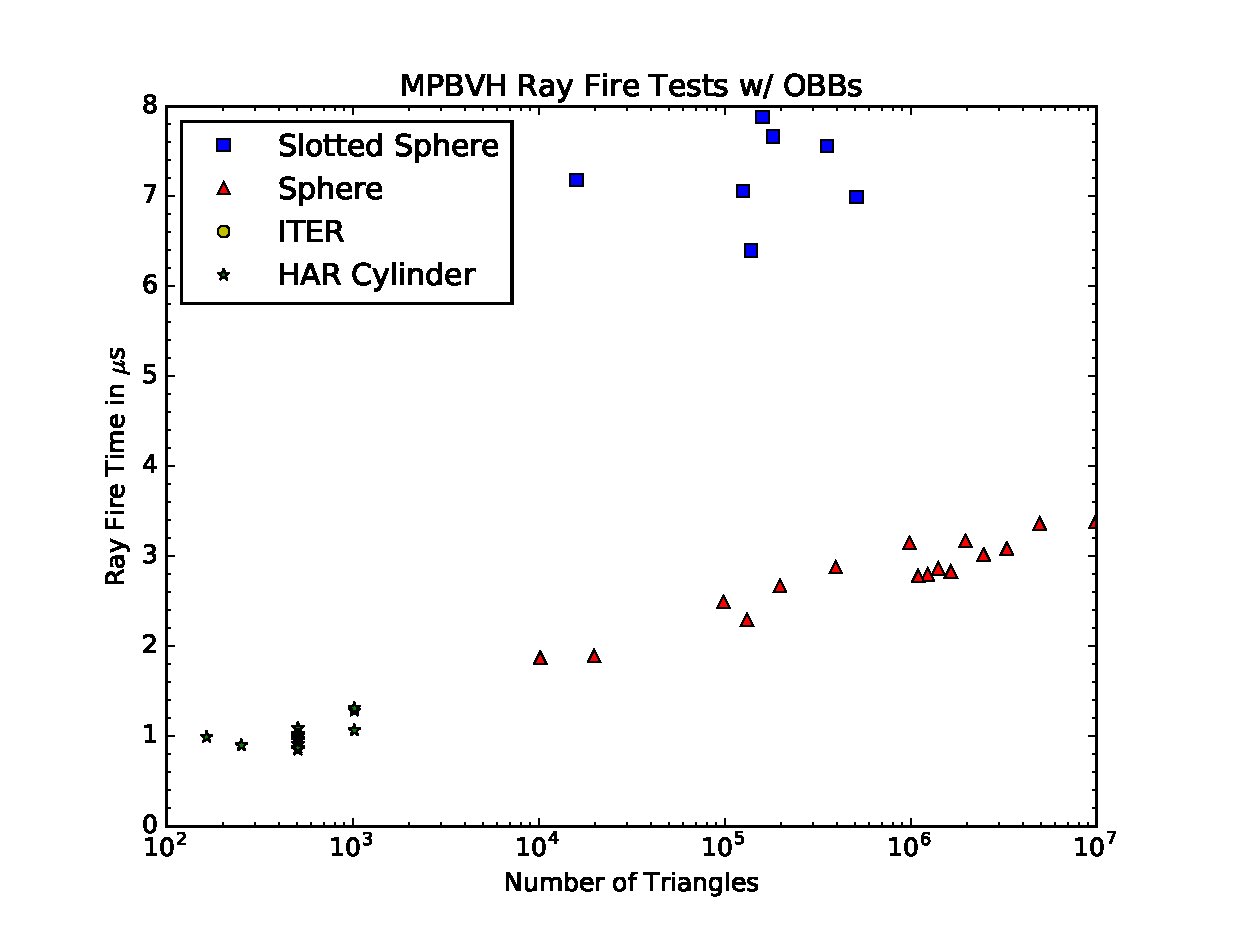
\includegraphics[scale=0.45]{mpbvh_rf_obb.eps}
  \caption{Ray fire tests on three representative DAGMC volume. Each data point
    represents the average ray fire time for 600k randomly directed rays from
    the origin of each volume. Top Left: Results of the tests for MOAB's OBB
    Tree. Top Right: Results of the tests for DAGMC coupled with Embree, or
    EmDAG. Bottom: Ray fire test results for DAGMC coupled with the MPBVH. The
    scale used for the MOAB OBB Tree is 10x greater than in the other two cases
    due to the slower speed.}
  \label{fig:rf_test_results_obbs}
\end{figure}

The combination of the MPBVH leaf examination in HV areas with the slower ray
fire times of OBBs lead to the hypothesis that OBBs can be beneficial to ray
fire times, but only if they are used in regions of the model where sibling
AABBs contain large overlaps.

\subsection{Adaptive Construction: Mixed AABB/OBBs}

The solution to HV regions when using the SIMD BVH
kernel proposed by the author is to apply OBBs only in regions determined to be
high valence using the same detection method described in Section
\ref{subsubsec:hv_detection}. Large leaf nodes being split into smaller nodes
will apply oriented bounding boxes to contain entities if the set of triangles
is determined to be a high valence region using the same method discussed in
Section \ref{subsubsec:hv_detection}.  The results using the mixed tree with
OBBs applied in HV regions are shown in Figure \ref{fig:simd_hv_studies}. The
mixed tree implementation shows some proportional scaling with both area
fraction and valence, but overall timing is significantly better, with the worst
case timing still beating out the best case for the OBB only characterization
test. This indicates that the AABBs are accelerating intersections higher up in
the tree while the OBBs resolve the high valence region with minimal overlap,
resulting in an overall improvement in the runtimes for these regions.

\subsubsection{Multi-Node Encoding}

To support a tree containing both AABBs and OBBs, additional encoding of
interior nodes is required so that the appropriate node intersection methods are
applied during traversal. Axis-Aligned and Oriented nodes are identiifed using
the the two remaining bit configurations available for node definitions by
setting the appropriate bits in the node reference objects. These node masks are
stripped from the node reference's integer value to retrieve the pointer to the
node objects themselves with little added overhead in the traversal process.

\section{Transport Testing}

The Mixed MPBVH was applied to the same set of production transport tests as the
AABB MPBVH in Section \ref{subsec:mpbvh_production_transport}. Timing resuls of
these simulations can be found in Figure \ref{fig:hv_parameter_study_simd}.

\begin{figure}[H]
  \centering
  \includesvg{../images/hv_parameter_study_simd}{1.0\textwidth}
  \caption{Variation in runtime for different HV detection parameters on a
    representative set of DAGMC models.}
  \label{fig:hv_parameter_study_simd}
\end{figure}

The application of OBBs in HV regions makes little difference in the simulation
runtimes of ATR or UWNR, but in the FNG model and ITER model the runtimes are
reduced by up to nearly 30\% with little additional build times in the BVH and
minimal increase in the memory footprint by replacing some of the AABBs with
OBBs.

The effect of the HV parameter on the build process makes it part of a splitting heuristic

\section{Conclusion}

This chapter introduced performance degredation caused by a tesselation feature
seen in engineering design models for radiation transport. A test model was then
developed to characterize and study the underlying cause of this degredation for
several ray tracing systems. In MOAB's OBB BVH, the main cause was leaf nodes
containing large numbers of triangles. The cause of poor ray tracing performance
in this system was a combination of the tree's design and default splitting
heuristic. A simple HV detection algorithm was presented and applied in a
solution where build settings of the splitting heuristic are adjusted for
portions of the tree bounding HV regions. This method was then verified to
remove performance degredation of ray tracing performance in these regions. A
similar process was then conducted for both EmDAG and MPBVH.

In the MPBVH, and presumably in EmDAG, the exclusive use of AABB nodes results
in large overlaps between child boxes. Many negative triangle intersection
results resulted from these overlaps, a similar effect to containing many
triangles in a single leaf node. The solution proposed and verified by the
author is the use of OBBs only in HV regions by applying the same HV detection
method as was used in the MOAB OBB tree. It is important to note, that this was
only possible in the MPBVH due to it's application alongside MOAB, a fully
formed mesh database. The use of mesh-specific concepts such as element
adjacencies makes this detection method simple and efficient. This work was not
duplicated in Embree due to the difficulty involved in obtainig the same set of
information and application of a mixed BVH for ray tracing on triangle elements.

Finally, a study of the adaptive build method to production models is presented
for understanding of the HV parameter's effect on simulation runtimes. Little
impact was found for some models while a significant reduction was seen in
others. These changes in runtime are proportional to both the area and valence
of the HV regions, which is predicted by the HV characterization tests in
Figures \ref{fig:moab_hv_studies} and \ref{fig:simd_hv_studies}. It was also was
found that these runtimes are significantly reduced despite the fact that a very
small number of rays are intersected with triangles in HV regions as shown in
Table MORE CAPITAL LETTERS HERE YUCK.


\chapter{Conclusion}\label{ch:conclusion}

\section{Impact on CAD-Based MCRT}

This work provides a set of methods and implementations which significantly
improves the performance of DAGMC's particle tracking capability. Performance
improvements varied from 30-500\% for all tests presented, without no change in
the results from unmodified DAGMC code.

The SDF implementation in DAGMC showed promising results for contrived test
cases, but at most provided a 30\% improvement in performance for production
models. The opportunity space for this data structure is limited, but the model
used to inform it's application has been varied for the majority of cases,
though some improvements could be made for locally small average chord length
values.

The Mixed Precision Bounding Volume Hierarchy (MPBVH) provides a robust method
for returning higher precision intersections suitable for engineering analysis
while exploiting CPU SIMD instructions for reduced precision bounding
entities. The implementation provided by the author demonstrates performance
comparable to single precision systems used for rendering with a significant
demonstrated impact on transport performance.

The use of a mixed AABB/OBB tree to improve performance for models containing
severe high valence regions by informing BVH construction using an associated
mesh database, MOAB, demonstrates the necessity of oriented bounding boxes for
optimal performance in DAGMC models.

\begin{table}[H]
  \small
  \centering
  \begin{tabular}{lc}
    Model & Ratio to Unmodified DAG-MCNP \\
    \multicolumn{2}{c}{SDF} \\
    ITER  & 1.16 \\
    nTOF  & 1.41 \\
    SHINE & 1.56 \\
    SHINE & 1.35 \\
    SNS   & 1.00 \\
    \multicolumn{2}{c}{MPBVH} \\
    FNG  & 2.09  \\
    ATR  & 4.56  \\
    UWNR & 2.87  \\
    ITER & 5.81  \\
  \end{tabular}
  \caption[A summary of performance improvements in this work]{A summary of the
    best-case performance improvements for modificed versions of DAG-MCNP in a
    series of production test cases.}
  \label{tab:the_rub}
\end{table}

The overall impact of this work on CAD-based Monte Carlo Radiation Transport is
summarized in Table \ref{tab:the_rub}. Coputational savings of 2x at a minimum
when applying the MPBVH were observed, with greater benefits of >5x seen in one
test case. For access to all open source code, raw data, and results presented
here please refer to FigShare archive \textbf{DOI\_HERE}.

\section{Broader Impacts}\label{sec:other_contrib}

Broader impacts of this work include a performant CPU ray tracer capable of
use in engineering analysis work. The MPBVH is coupled with MOAB, a mesh
database currently in use for engineering analysis purposes at Argonne National
Lab. This tool can be built using standard GNU compilers and is relatively
lightweight.

Work on adaptive BVH construction around HV regions demonstrates the importance
of spatial query capabilities which are closely linked to a mesh framework in
order to be able to detect problematic mesh features and adjust build settings.

The use of a mixed AABB/OBB to improve performance for models containing high
valence regions suggests that for engineering analysis, or at least for the
surface meshses generated by Cubit/Trelis for use in DAGMC, that AABBs can cause
large amounts of overlap in certain regions of the model, resulting in several
orders of magnitude degradation in ray query times.

\section{Suggested Future Work}\label{sec:future_work}

Some improvement of the SDF model is suggested in which additional information
about the geometric properties of the target volume is used to inform decisions
about SDF application. In particular, information on the variation of the
average chord length could be used to avoid application of the data structure
where its predicted utilization is over estimated. Spatially varying information
on the collision density of particles, could also be used to better inform the
predictive tool for analysis.

Another extension of the SDF predictive model could be its use to inform
algorithms for domain subdivision in codes where Woodcock delta tracking is
applied \cite{Leppanen_2010} \cite{Yonghao_2011}. 

There are many directions work on the MPBVH could take. Slightly more exotic
architectures used in high performance computing clusters provide wider
registers than the AVX2 instructions used in this work. This creates the
possibility of creating tree branching ratio of 8 or 16 for even more shallow
trees and lower memory footprints. Higher branching ratios also allow the MPBVH
to extend naturally to other hierarchies like the Octree which has other
benefits in particle tracking and data field storage.

As suggested in Chapter \ref{ch:simd_bvh}, box extension values could be applied
on a volume-by-volume basis for MCRT to avoid performance degradation in models
with a large global scale, but regions with small components. This is
application-specific, but could be integrated into the interface of the MPBVH
to be set according to different use-cases.

Mesh features similar to the high valence region could be sought out using a
variety of meshing schemes, geometries, and a program designed to highlight
regions of models in which ray fire times are much lower than average to
automatically highlight these areas for characterization and analysis as was
done for the high valence region. 



% 
\section{Motivation}

\begin{frame}
  \frametitle{CAD-Based Monte Carlo}
\end{frame}

% \include{related/related}

%% etc, etc.

%% Do you have appendices?  If so, add them here, just like chapters.
\begin{appendices}
  
\chapter{Appendix A: Modified-BVH DAGMC Simulation Results}\label{ch:appendix_a}

This appendix contains all results for simulations performed using modified or
replaced ray tracing kernels such as the EmDAG or MPBVH systems.

\section{EmDAG}

\subsection{Simple Test Cases}

\begin{table}[H]
  \small
  \begin{center}
    \begin{tabular}{lccc}
      \toprule
      Value & MCNP & DAG-MCNP & EmDAG-MCNP \\
      \toprule
      %%Hist/min & 2.2991E+05 & 1.9877E+04 & 1.3947E+05 \\
      %%\hline
      \multicolumn{4}{l}{\textbf{Cell 1 Tallies}} \\
      \hline
      Flux  & 5.25725E-03 & 5.25734E-03 & 5.25734E-03 \\
      Energy  & 3.17869E-03 &  3.17873E-03 &  3.17873E-03 \\
      \hline
      \multicolumn{4}{l}{\textbf{Cell 2 Tallies}} \\
      \hline
      Flux  & 1.91645E-04 & 1.91644E-04 & 1.91644E-04 \\
      Energy  & 5.22131E-05 & 5.22137E-05 & 5.22137E-05 \\
      \hline
      \multicolumn{4}{l}{\textbf{Cell 3 Tallies}} \\
      \hline
      Flux  & 1.18371E-05 & 1.18376E-05 & 1.18410E-05 \\
      Energy  & 4.96282E-06 & 4.96285E-06 & 4.96285E-06 \\
      \bottomrule
                        
    \end{tabular}
    \caption{Nested Spheres Tally Results. Flux tally units are
      $cm^{-2}$. Energy tally units are MeV/g. Note: result comparisons of other
      test cases can be found in Appendix B.}
    \label{nestedspheres}
  \end{center}
%%\vspace{-0.2cm}
\end{table}



  \include{chapters/08-appendix_b}
\end{appendices}

%% Are you a big nerd with a colophon?  Add it here.
%% \begin{colophon}
%% \svnidlong{$LastChangedBy$}{$LastChangedRevision$}{$LastChangedDate$}{$HeadURL: http://freevariable.com/dissertation/trunk/frontmatter.tex $}
\vcinfo{}

This template uses Gyre Pagella by default.  (I used Arno Pro in my dissertation.)

Feel free to give me a shout-out in your colophon or acks if this template is useful for you.  Good luck!

%% \end{colophon}

%% McBride is a very nice style (some version is included in this distribution)
\bibliographystyle{mcbride}
\bibliography{refs}

%% Want an index?  Neither did I.
%\printindex

\end{document}
